% Document maitre -- EPD-GIT-5534, les 6 seances
% =====================================================================
%  EPD-GIT-5534 -- Apprentissage automatique applique aux infrastructures
%  Preambule commun aux seances
%  Moteur : XeLaTeX (Tectonic) -- compilation : voir build.py
% =====================================================================
\documentclass[10pt,aspectratio=169]{beamer}

\usepackage{fontspec}
\usepackage{polyglossia}
\setdefaultlanguage{french}
\usepackage{amsmath,amssymb,mathtools}
\usepackage{unicode-math}
\usepackage{booktabs}
\usepackage{array}
\usepackage{colortbl}
\usepackage{xcolor}
\usepackage{tikz}
\usetikzlibrary{arrows.meta,positioning,calc,shapes.geometric,fit,backgrounds,patterns}
\usepackage{pgfplots}
\pgfplotsset{compat=1.18}
\usepgfplotslibrary{fillbetween}
\usepackage{graphicx}
\usepackage{listings}
\usepackage[most]{tcolorbox}
\tcbuselibrary{skins,breakable}
\usepackage{fontawesome5}
\usepackage{multicol}
\usepackage{multirow}
\usepackage{animate}

% ---------------------------------------------------------------- theme
\usetheme{default}
\usecolortheme{default}
\setbeamertemplate{navigation symbols}{}

\definecolor{byDeep}   {HTML}{10243E}
\definecolor{byBlue}   {HTML}{1F6FEB}
\definecolor{byCyan}   {HTML}{12A594}
\definecolor{byOrange} {HTML}{D97706}
\definecolor{byRed}    {HTML}{C0392B}
\definecolor{byGreen}  {HTML}{1E8449}
\definecolor{byPurple} {HTML}{6C5CE7}
\definecolor{byGrey}   {HTML}{5B6470}
\definecolor{byLight}  {HTML}{F4F6F8}

\setbeamercolor{frametitle}{bg=byDeep,fg=white}
\setbeamercolor{structure}{fg=byBlue}
\setbeamercolor{normal text}{fg=byDeep}
\setbeamercolor{alerted text}{fg=byRed}
\setbeamercolor{title}{fg=white}
\setbeamercolor{subtitle}{fg=white}
\setbeamercolor{author}{fg=white}
\setbeamercolor{date}{fg=white}
\setbeamercolor{item}{fg=byBlue}
\setbeamercolor{section in toc}{fg=byDeep}
\setbeamercolor{block title}{bg=byBlue!12,fg=byDeep}
\setbeamercolor{block body}{bg=byBlue!5}

\setbeamerfont{frametitle}{size=\large,series=\bfseries}
\setbeamerfont{title}{size=\LARGE,series=\bfseries}
\setbeamerfont{block title}{series=\bfseries}

% gain de place vertical : le titre de frame est suivi d'un espace negatif
% (les supports sont denses ; cela evite que le dernier encadre morde sur le pied de page)
\addtobeamertemplate{frametitle}{}{\vspace*{-4.0mm}}
\setlength{\abovedisplayskip}{3pt}
\setlength{\belowdisplayskip}{3pt}
\setlength{\abovedisplayshortskip}{2pt}
\setlength{\belowdisplayshortskip}{2pt}

\setbeamertemplate{itemize item}{\small\raise0.2ex\hbox{\textcolor{byBlue}{$\blacktriangleright$}}}
\setbeamertemplate{itemize subitem}{\tiny\raise0.35ex\hbox{\textcolor{byCyan}{$\bullet$}}}
\setlength{\tabcolsep}{3pt}   % tableaux plus etroits (les slides sont denses)
% listes plus compactes : les supports sont denses et le pied de page mange de la place
\setbeamertemplate{itemize/enumerate body begin}{\vspace*{-2.0mm}}
\setbeamertemplate{itemize/enumerate subbody begin}{\vspace*{-0.6mm}}
\setbeamertemplate{enumerate item}{\textcolor{byBlue}{\bfseries\insertenumlabel.}}
\setbeamertemplate{caption}[numbered]

% footer : chapitre | slide n/N
\setbeamertemplate{footline}{%
  % Beamer reserve la hauteur de cette boite comme zone interdite : le vskip
  % ci-dessous cale la zone de texte exactement au-dessus de la barre visible.
  \vskip 10mm%
  \leavevmode%
  \hbox{%
    \begin{beamercolorbox}[wd=.32\paperwidth,ht=1.9ex,dp=0.8ex,leftskip=.3cm]{author in head/foot}%
      \usebeamerfont{author in head/foot}\color{white}\scriptsize\insertshorttitle
    \end{beamercolorbox}%
    \begin{beamercolorbox}[wd=.52\paperwidth,ht=1.9ex,dp=0.8ex,center]{title in head/foot}%
      \usebeamerfont{title in head/foot}\color{white}\scriptsize Par Dr. Noulapeu Ngaffo Armielle
    \end{beamercolorbox}%
    \begin{beamercolorbox}[wd=.16\paperwidth,ht=1.9ex,dp=0.8ex,rightskip=.3cm]{date in head/foot}%
      \usebeamerfont{date in head/foot}\color{white}\scriptsize\insertframenumber\,/\,\inserttotalframenumber
    \end{beamercolorbox}}%
  \vskip0pt%
}
\setbeamercolor{author in head/foot}{bg=byDeep}
\setbeamercolor{title in head/foot}{bg=byDeep!88}
\setbeamercolor{date in head/foot}{bg=byDeep!76}

\setbeamertemplate{title page}{%
  \begin{tikzpicture}[remember picture,overlay]
    \fill[byDeep] (current page.north west) rectangle (current page.south east);
    \fill[byBlue,opacity=.30] (current page.north east) ++(-3.2,-1.1) circle (5.4cm);
    \fill[byCyan,opacity=.18] (current page.south west) ++(2.2,1.0) circle (4.2cm);
  \end{tikzpicture}
  \vspace{1.1cm}
  \begin{center}
    {\usebeamerfont{title}\usebeamercolor[fg]{title}\inserttitle\par}
    \vspace{.25cm}
    {\large\color{byCyan}\insertsubtitle\par}
    \vspace{.7cm}
    {\color{white}\small\insertauthor\par}
    \vspace{.15cm}
    {\color{white!80}\footnotesize\insertinstitute\par}
    \vspace{.15cm}
    {\color{white!70}\footnotesize\insertdate\par}
  \end{center}
}

% ------------------------------------------------------- boites maison
\newtcolorbox{qbox}[1][QUIZ]{%
  enhanced,colback=byOrange!7,colframe=byOrange,boxrule=.9pt,arc=2mm,
  left=2mm,right=2mm,top=3.4mm,bottom=1.2mm,
  title={\faQuestionCircle\ \bfseries #1},fonttitle=\bfseries\scriptsize\color{white},
  colbacktitle=byOrange,attach boxed title to top left={xshift=3mm,yshift=-2mm},
  boxed title style={arc=1mm,boxrule=0pt}}

\newtcolorbox{abox}[1][ACTIVITE]{%
  enhanced,colback=byBlue!6,colframe=byBlue,boxrule=.9pt,arc=2mm,
  left=2mm,right=2mm,top=3.4mm,bottom=1.2mm,
  title={\faUsers\ \bfseries #1},fonttitle=\bfseries\scriptsize\color{white},
  colbacktitle=byBlue,attach boxed title to top left={xshift=3mm,yshift=-2mm},
  boxed title style={arc=1mm,boxrule=0pt}}

\newtcolorbox{ebox}[1][EXEMPLE]{%
  enhanced,colback=byGreen!6,colframe=byGreen,boxrule=.9pt,arc=2mm,
  left=2mm,right=2mm,top=3.4mm,bottom=1.2mm,
  title={\faFlask\ \bfseries #1},fonttitle=\bfseries\scriptsize\color{white},
  colbacktitle=byGreen,attach boxed title to top left={xshift=3mm,yshift=-2mm},
  boxed title style={arc=1mm,boxrule=0pt}}

\newtcolorbox{kbox}[1][A RETENIR]{%
  enhanced,colback=byPurple!6,colframe=byPurple,boxrule=.9pt,arc=2mm,
  left=2mm,right=2mm,top=3.4mm,bottom=1.2mm,
  title={\faLightbulb\ \bfseries #1},fonttitle=\bfseries\scriptsize\color{white},
  colbacktitle=byPurple,attach boxed title to top left={xshift=3mm,yshift=-2mm},
  boxed title style={arc=1mm,boxrule=0pt}}

\newtcolorbox{wbox}[1][ATTENTION]{%
  enhanced,colback=byRed!6,colframe=byRed,boxrule=.9pt,arc=2mm,
  left=2mm,right=2mm,top=3.4mm,bottom=1.2mm,
  title={\faExclamationTriangle\ \bfseries #1},fonttitle=\bfseries\scriptsize\color{white},
  colbacktitle=byRed,attach boxed title to top left={xshift=3mm,yshift=-2mm},
  boxed title style={arc=1mm,boxrule=0pt}}

\newtcolorbox{solbox}[1][SOLUTION]{%
  enhanced,colback=byCyan!7,colframe=byCyan,boxrule=.9pt,arc=2mm,
  left=2mm,right=2mm,top=3.4mm,bottom=1.2mm,
  title={\faCheckCircle\ \bfseries #1},fonttitle=\bfseries\scriptsize\color{white},
  colbacktitle=byCyan,attach boxed title to top left={xshift=3mm,yshift=-2mm},
  boxed title style={arc=1mm,boxrule=0pt}}

\newtcolorbox{codebox}[1][Code Python]{%
  enhanced,colback=byLight,colframe=byGrey!60,boxrule=.6pt,arc=1.5mm,
  left=1.5mm,right=1.5mm,top=3.8mm,bottom=1.0mm,
  title={\faPython\ \ttfamily\small #1},fonttitle=\small\color{white},
  colbacktitle=byGrey,attach boxed title to top left={xshift=3mm,yshift=-2mm},
  boxed title style={arc=1mm,boxrule=0pt}}

\newtcolorbox{figbox}[1][]{%
  enhanced,colback=white,colframe=byDeep!25,boxrule=.6pt,arc=1.5mm,
  left=1mm,right=1mm,top=1mm,bottom=1mm,#1}

% --------------------------------------------------------- listings
\definecolor{codekw}{HTML}{0B5394}
\definecolor{codestr}{HTML}{B8531A}
\definecolor{codecom}{HTML}{57744E}
\definecolor{codebg}{HTML}{F6F8FA}
\lstdefinestyle{py}{
  language=Python,
  backgroundcolor=\color{codebg},
  basicstyle=\ttfamily\fontsize{6.6}{7.6}\selectfont,
  keywordstyle=\color{codekw}\bfseries,
  commentstyle=\color{codecom}\itshape,
  stringstyle=\color{codestr},
  numberstyle=\tiny\color{byGrey},
  numbers=left,numbersep=4pt,
  frame=none,
  breaklines=true,breakatwhitespace=false,
  showstringspaces=false,
  columns=fullflexible,keepspaces=true,
  upquote=true,
  literate={é}{{\'e}}1 {è}{{\`e}}1 {ê}{{\^e}}1 {à}{{\`a}}1 {â}{{\^a}}1
           {î}{{\^i}}1 {ô}{{\^o}}1 {û}{{\^u}}1 {ç}{{\c c}}1 {ù}{{\`u}}1
           {É}{{\'E}}1 {È}{{\`E}}1 {À}{{\`A}}1 {Ê}{{\^E}}1 {Ç}{{\c C}}1
           {œ}{{\oe}}1 {’}{{'}}1 {«}{{\guillemotleft}}1 {»}{{\guillemotright}}1
           {→}{{$\rightarrow$}}1 {α}{{$\alpha$}}1 {β}{{$\beta$}}1 {θ}{{$\theta$}}1
           {μ}{{$\mu$}}1 {σ}{{$\sigma$}}1 {λ}{{$\lambda$}}1 {π}{{$\pi$}}1
           {τ}{{$\tau$}}1 {ρ}{{$\rho$}}1 {≈}{{$\approx$}}1 {≤}{{$\leq$}}1
           {≥}{{$\geq$}}1 {×}{{$\times$}}1 {≠}{{$\neq$}}1 {∈}{{$\in$}}1
}
\lstset{style=py}

\newcommand{\py}[1]{\lstinline[style=py,basicstyle=\ttfamily\small]|#1|}
\newcommand{\file}[1]{\texttt{\small #1}}
\newcommand{\R}{\mathbb{R}}
\newcommand{\N}{\mathcal{N}}
\newcommand{\E}{\mathbb{E}}
\newcommand{\Var}{\mathrm{Var}}
\newcommand{\post}{\text{post}}
\newcommand{\like}{\text{vrais.}}
\newcommand{\data}{\mathcal{D}}
\newcommand{\given}{\,\vert\,}
\DeclareMathOperator*{\argmax}{arg\,max}
\DeclareMathOperator*{\argmin}{arg\,min}

% icones de validation
\newcommand{\ok}{\textcolor{byGreen}{\faCheckCircle}}
\newcommand{\nok}{\textcolor{byRed}{\faTimesCircle}}
\newcommand{\warn}{\textcolor{byOrange}{\faExclamationTriangle}}

% chemin des figures
\graphicspath{{../figures/}{./figures/}{figures/}{../assets/}{./assets/}}

% ------------------------------------------------ page de garde de chapitre
% A utiliser en tete de chaque fichier de chapitre : identique en build
% autonome et en build maitre (aucune dependance a \title).
\newcommand{\chapterslide}[4]{%
\begin{frame}[plain]
\begin{tikzpicture}[remember picture,overlay]
  \fill[byDeep] (current page.north west) rectangle (current page.south east);
  \fill[byBlue,opacity=.30] (current page.north east) ++(-3.0,-0.9) circle (5.0cm);
  \fill[byCyan,opacity=.16] (current page.south west) ++(2.4,1.2) circle (4.4cm);
\end{tikzpicture}
\vspace{0.55cm}
\begin{columns}[c]
% ---- logo officiel de l'ecole, dans un cartouche blanc
\begin{column}{0.20\textwidth}
  \centering
  \begin{tcolorbox}[colback=white,colframe=white,boxrule=0pt,arc=1.5mm,
     left=1mm,right=1mm,top=1mm,bottom=1mm,width=2.5cm]
    \centering
    
\includegraphics[width=2.1cm]{logo_enspd.png}
  \end{tcolorbox}
\end{column}
% ---- identification du chapitre et de l'enseignante
\begin{column}{0.76\textwidth}
  {\color{byCyan}\bfseries\large #1\par}
  \vspace{.20cm}
  {\color{white}\bfseries\Large #2\par}
  \vspace{.30cm}
  {\color{white!85}\small Apprentissage automatique appliqué aux infrastructures --- EPD-GIT-5534\par}
  \vspace{.06cm}
  {\color{white!70}\footnotesize #3\par}
  \vspace{.26cm}
  {\color{byCyan}\bfseries\normalsize Enseignante : Dr. Noulapeu Ngaffo Armielle\par}
  \vspace{.06cm}
  {\color{white!80}\footnotesize École Nationale Supérieure Polytechnique de Douala\par}
  {\color{white!65}\footnotesize Université de Douala --- Département Génie Informatique
   et Télécommunications\par}
\end{column}
\end{columns}
\vspace{.30cm}
\begin{columns}[t]
\begin{column}{0.06\textwidth}\end{column}
\begin{column}{0.88\textwidth}
\begin{tcolorbox}[enhanced,colback=byDeep!62!black,colframe=byCyan!75,arc=2mm,
   boxrule=.6pt,left=2mm,right=2mm,top=1.4mm,bottom=1.4mm,coltext=white]
\small #4
\end{tcolorbox}
\end{column}
\begin{column}{0.06\textwidth}\end{column}
\end{columns}
\end{frame}}

% compteur de slides atteignables : \nb{50}
\newcommand{\nb}[1]{}


\title[EPD-GIT-5534 --- Support complet]{Apprentissage automatique appliqué aux infrastructures}
\subtitle{EPD-GIT-5534 --- Support complet : 6 séances de 4 h (30 h, 3 crédits)}
\author{Enseignante : Dr. Noulapeu Ngaffo Armielle}
\institute{Département Génie Informatique et Télécommunications}
\date{Année universitaire 2026--2027}
\begin{document}
\begin{frame}[plain]
\begin{tikzpicture}[remember picture,overlay]
  \fill[byDeep] (current page.north west) rectangle (current page.south east);
  \fill[byBlue,opacity=.30] (current page.north east) ++(-3.0,-0.9) circle (5.0cm);
  \fill[byCyan,opacity=.16] (current page.south west) ++(2.4,1.2) circle (4.4cm);
\end{tikzpicture}
\vspace{0.9cm}
\begin{center}
{\color{white}\bfseries\LARGE Apprentissage automatique\\[1mm] appliqué aux infrastructures\par}
\vspace{.35cm}
{\color{byCyan}\large EPD-GIT-5534 --- Support complet\par}
\vspace{.5cm}
{\color{white!85}\small 6 séances de 4 h --- 2 h cours + 2 h TP --- 30 h, 3 crédits\par}
\vspace{.55cm}
{\color{byCyan}\bfseries\normalsize Enseignante : Dr. Noulapeu Ngaffo Armielle\par}
\vspace{.1cm}
{\color{white!80}\footnotesize École Nationale Supérieure Polytechnique de Douala\par}
{\color{white!65}\footnotesize Université de Douala --- Département Génie Informatique et Télécommunications\par}
\end{center}
\end{frame}
\begin{frame}{Sommaire du support}
\begin{columns}[t]
\begin{column}{0.48\textwidth}
\begin{enumerate}
\item \textbf{Séance 1} --- Introduction au ML et aux infrastructures
\item \textbf{Séance 2} --- Données d'infrastructures et préparation
\item \textbf{Séance 3} --- Modèles de ML appliqués aux infrastructures
\end{enumerate}
\end{column}
\begin{column}{0.48\textwidth}
\begin{enumerate}\setcounter{enumi}{3}
\item \textbf{Séance 4} --- Supervision, optimisation et prédiction
\item \textbf{Séance 5} --- Sécurité et fiabilité des infrastructures assistées par l'IA
\item \textbf{Séance 6} --- Perspectives, évolutions et industrialisation
\end{enumerate}
\end{column}
\end{columns}
\vspace{2mm}
\begin{kbox}[Fil conducteur]
\textbf{NOSYS}, exploitant d'un centre de données et d'un réseau 4G/5G à Douala :
comprendre la plateforme $\to$ préparer les données $\to$ modéliser $\to$
prédire les pannes $\to$ détecter les intrusions $\to$ industrialiser.
\end{kbox}
\begin{center}\small
Évaluation : continue 30 \% (6 livrables) · TPE 20 \% · examen final 50 \% (1 h 30, 6 exercices).
\end{center}
\end{frame}
% =====================================================================
%  Seance 1 -- A. page de garde, plan, ML fondamental (frames 1--13)
% =====================================================================
\section{Séance 1 --- Introduction au ML et aux infrastructures}
\chapterslide{Séance 1}{Introduction à l'apprentissage automatique et aux infrastructures}
{4 h --- 2 h cours / 2 h TP --- Partie 1 du syllabus EPD-GIT-5534}
{\textbf{Objectifs :} situer les trois familles de ML $\bullet$ nommer les composants d'une
infrastructure et leurs indicateurs de santé (SLI/SLO/SLA, MTBF/MTTR) $\bullet$
formuler un problème opérationnel en termes de ML $\bullet$ explorer un jeu de
métriques réelles (NOSYS) et produire une fiche « état des lieux » chiffrée.}

\begin{frame}{Plan de la séance (4 h)}
\begin{columns}[t]
\begin{column}{0.48\textwidth}
\begin{kbox}[Cours magistral --- 2 h]
\begin{enumerate}
\item \textbf{Notions fondamentales du ML} (50 min) : les trois familles, le vocabulaire.
\item \textbf{Anatomie d'une infrastructure} (40 min) : couches, métriques, SLI/SLO/SLA, MTBF/MTTR.
\item \textbf{Le croisement : AIOps} (20 min) : pourquoi le ML change la supervision.
\item \textbf{Lancement du dossier NOSYS} (10 min).
\end{enumerate}
\end{kbox}
\end{column}
\begin{column}{0.48\textwidth}
\begin{ebox}[Travaux pratiques --- 2 h]
\textbf{« Cartographier la plateforme »} sur les vraies métriques
\file{nosys\_metriques.csv} :
\begin{enumerate}
\item B1 --- chargement et vérifications (30 min)
\item B2 --- inventaire de qualité (20 min)
\item B3 --- visualiser un serveur sur 7 jours (30 min)
\item B4 --- statistiques par serveur (40 min)
\item B5 --- livrable : fiche « état des lieux » (20 min)
\end{enumerate}
\end{ebox}
\end{column}
\end{columns}
\vspace{1mm}
\begin{center}\small
Fil conducteur des 6 séances : \textbf{NOSYS}, exploitant d'un centre de données
et d'un réseau 4G/5G à Douala.
\end{center}
\end{frame}

\begin{frame}{Pourquoi le ML change le métier d'exploitant}
\footnotesize%
\begin{columns}[t]
\begin{column}{0.52\textwidth}
\begin{ebox}[Le problème NOSYS (données réelles du dossier)]
Les journaux du mois (\file{nosys\_logs.csv}) contiennent \textbf{100\,000 lignes}
d'authentification. Une intrusion brute force y est enfouie :
\textbf{125 échecs d'authentification concentrés} sur 2 heures de nuit,
sur les comptes \py{root}, \py{admin}, \py{inconnu-*}.
\begin{itemize}
\item Baseline normale : $\approx$ 30 échecs/jour sur tout le parc.
\item Personne ne lit 100\,000 lignes : \textbf{l'œil humain rate l'attaque}.
\end{itemize}
\end{ebox}
\begin{kbox}[La promesse de cette UE]
Un modèle qui lit les données en continu, apprend ce qui est \emph{normal},
et alerte \emph{avant} la panne --- pas 3 heures après.
\end{kbox}
\end{column}
\begin{column}{0.44\textwidth}
\begin{wbox}[Ce que le ML ne remplace pas]
\begin{itemize}
\item Le \textbf{bon sens opérationnel} : un modèle alerte, un humain décide.
\item Les \textbf{règles simples} quand elles suffisent (un disque plein, on le voit).
\item La \textbf{qualité des données} : garbage in, garbage out.
\end{itemize}
\end{wbox}
\vspace{2mm}
\begin{center}\small
Objectifs pédagogiques du syllabus couverts aujourd'hui :\\
\#1 concepts fondamentaux $\bullet$ \#2 usages dans les infrastructures.
\end{center}
\end{column}
\end{columns}
\end{frame}

\begin{frame}{Qu'est-ce que l'apprentissage automatique ?}
\begin{block}{Définition de travail}
\textbf{Apprendre} une fonction de prédiction ou de structure
$f$ à partir de \textbf{données}, plutôt que de l'écrire à la main :
\[
\text{données } (x, y) \;\longrightarrow\; \text{apprentissage}
\;\longrightarrow\; f \;\longrightarrow\; \text{prédictions sur du \textbf{nouveau}}
\]
\end{block}
\begin{itemize}
\item \textbf{Programmation classique} : l'humain écrit les règles
(\py{if cpu > 90: alerte()}).
\item \textbf{ML} : l'humain fournit des exemples, la machine \emph{apprend} les règles
--- y compris celles qu'on ne saurait pas écrire (quel pattern de latence annonce une panne ?).
\item Le critère d'apprentissage (fonction de coût) et la mesure de généralisation
sont les \textbf{deux piliers} de tout modèle : on les verra à chaque séance.
\end{itemize}
\begin{kbox}[À retenir dès maintenant]
Un modèle vaut ce que vaut sa performance \textbf{sur des données qu'il n'a jamais vues}
--- jamais sa performance sur les données d'entraînement.
\end{kbox}
\end{frame}

\begin{frame}{Les trois familles de l'apprentissage}
\footnotesize%
\begin{center}
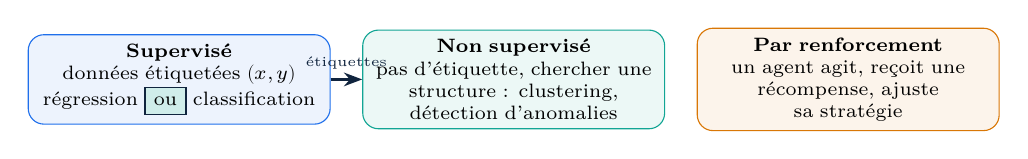
\begin{tikzpicture}[node distance=4mm,
  box/.style={rectangle,rounded corners=2mm,draw,align=center,font=\scriptsize,minimum height=9mm}]
\node[box,draw=byBlue,fill=byBlue!8,text width=3.6cm] (sup) {\textbf{Supervisé}\\données étiquetées $(x,y)$\\régression \fcolorbox{byDeep}{byCyan!20}{\scriptsize ou} classification};
\node[box,draw=byCyan,fill=byCyan!8,right=of sup,text width=3.6cm] (nonsup) {\textbf{Non supervisé}\\pas d'étiquette, chercher une\\structure : clustering,\\détection d'anomalies};
\node[box,draw=byOrange,fill=byOrange!8,right=of nonsup,text width=3.6cm] (renf) {\textbf{Par renforcement}\\un agent agit, reçoit une\\récompense, ajuste\\sa stratégie};
\draw[-{Stealth},thick,byDeep] (sup) -- node[above,font=\tiny]{étiquettes} (nonsup);
\end{tikzpicture}
\end{center}
\vspace{1mm}
\begin{columns}[t]
\begin{column}{0.32\textwidth}
\begin{ebox}[En infrastructure]
Prédire la latence à $h{+}1$ ;\\
classer une session « attaque / légitime » ;\\
estimer la durée d'un incident.
\end{ebox}
\end{column}
\begin{column}{0.32\textwidth}
\begin{ebox}[En infrastructure]
Regrouper les serveurs par profil de charge ;\\
détecter les fenêtres « anormales » ;\\
segmenter les applications.
\end{ebox}
\end{column}
\begin{column}{0.32\textwidth}
\begin{ebox}[En infrastructure]
Piloter le refroidissement d'une salle ;\\
ajuster dynamiquement la\\limite de débit d'un client.
\end{ebox}
\end{column}
\end{columns}
\vspace{1mm}
\begin{center}\small
Cette UE couvre en profondeur les \textbf{deux premières familles} ;
le renforcement est un aperçu culturel.
\end{center}
\end{frame}

\begin{frame}{Supervisé (1/2) : la régression}
\footnotesize%
\begin{block}{Principe}
La cible $y$ est \textbf{continue}. On apprend $f(x) \approx y$, par exemple une forme linéaire
\[
\hat{y} = \beta_0 + \beta_1 x_1 + \dots + \beta_p x_p
\]
en minimisant l'erreur quadratique moyenne (MSE) :
\[
\mathrm{MSE} = \frac{1}{n}\sum_{i=1}^{n}\bigl(y_i - \hat{y}_i\bigr)^2
\]
\end{block}
\begin{columns}[t]
\begin{column}{0.48\textwidth}
\begin{ebox}[Exemples « infrastructure »]
\begin{itemize}
\item Prédire la \textbf{latence} de demain 14 h--15 h à partir de la charge.
\item Prédire la \textbf{consommation} (kWh) d'une salle la semaine prochaine
--- notre parc a consommé \textbf{11\,614 kWh} en 30 jours : le modèle du TP de la
séance 4 partira de ce chiffre.
\item Estimer la \textbf{durée restante} avant saturation du stockage.
\end{itemize}
\end{ebox}
\end{column}
\begin{column}{0.48\textwidth}
\begin{kbox}[Ce qu'on apprendra (séances 4 et 11)]
\begin{itemize}
\item Régression linéaire : interpréter un $\beta$ (« +1 \% de CPU $\Rightarrow$ +x ms »).
\item Séries temporelles (ARIMA) : les métriques d'infra sont \textbf{correlées dans le temps},
on ne peut pas les traiter comme un tableau aléatoire.
\end{itemize}
\end{kbox}
\end{column}
\end{columns}
\end{frame}

\begin{frame}{Supervisé (2/2) : la classification}
\footnotesize%
\begin{block}{Principe}
La cible $y$ est \textbf{discrète} (une classe). Le modèle sort une \textbf{probabilité}
$P(y = k \given x)$ et une règle de décision (seuil).
\[
P(\text{incident} \given \text{CPU, latence, heure}) = 0{,}87
\;\Rightarrow\; \text{alerte si } P > 0{,}5
\]
\end{block}
\begin{columns}[t]
\begin{column}{0.48\textwidth}
\begin{ebox}[Exemples « infrastructure »]
\begin{itemize}
\item \textbf{Incident dans les 30 min ?} (cible binaire, construite au TP2)
\item \textbf{Session attaque / légitime} (séance 5)
\item \textbf{Triage} d'un ticket : réseau / matériel / applicatif
\end{itemize}
\end{ebox}
\begin{wbox}[Le piège des classes rares]
Les incidents sont rares (16 blocs sur un mois) : la simple
\textbf{exactitude} est trompeuse. Un modèle qui dit toujours
« pas d'incident » a 99,98 \% d'exactitude et \textbf{zéro valeur}.
$\Rightarrow$ précision, rappel, F1 (séance 3).
\end{wbox}
\end{column}
\begin{column}{0.48\textwidth}
\begin{kbox}[Vocabulaire de décision]
\begin{itemize}
\item \textbf{Faux positif} : alerte injustifiée $\Rightarrow$ fatigue d'alerte du NOC.
\item \textbf{Faux négatif} : panne non détectée $\Rightarrow$ SLA cassé.
\item Les deux coûts sont \textbf{asymétriques} : c'est un choix métier, pas technique.
\end{itemize}
\end{kbox}
\end{column}
\end{columns}
\end{frame}

\begin{frame}{Non supervisé : clustering et détection d'anomalies}
\footnotesize%
\begin{columns}[t]
\begin{column}{0.48\textwidth}
\begin{block}{Clustering}
Regrouper les observations \textbf{sans étiquette}. Ex. : $k$-means
partitionne les serveurs selon (CPU, RAM, latence) en $k$ profils.
\begin{itemize}
\item Sert à \textbf{comprendre} avant de modéliser.
\item Séance 10 (cours de ML général) / séance 5 ici pour regrouper des attaques.
\end{itemize}
\end{block}
\begin{ebox}[Sur NOSYS]
Classer nos \textbf{8 serveurs} par profil de charge : avec les CPU moyens
(14,4 à 24,6 \%), les profils sont proches --- le clustering devient intéressant
quand on agrège par \emph{application}, pas par machine.
\end{ebox}
\end{column}
\begin{column}{0.48\textwidth}
\begin{block}{Détection d'anomalies}
Apprendre la distribution du \textbf{normal}, puis mesurer l'improbabilité :
\[
\text{score}(x) \text{ grand}
\;\Longleftrightarrow\;
x \text{ improbable sous } p_{\text{norm}}
\]
\begin{itemize}
\item C'est \textbf{le} problème central de la supervision.
\item Outils de la séance 3 : $z$-score, IQR, isolation forest, LOF.
\end{itemize}
\end{block}
\begin{kbox}[Pourquoi pas seulement des seuils ?]
Parce que « normal » \textbf{dépend de l'heure} : CPU 30 \% à 14 h est normal,
CPU 30 \% à 3 h du matin pour srv-01 est suspect. Un seuil fixe ne voit pas cette différence.
\end{kbox}
\end{column}
\end{columns}
\end{frame}

\begin{frame}{Par renforcement : l'aperçu culturel}
\footnotesize%
\begin{block}{Principe}
Un \textbf{agent} observe un état, \textbf{agit}, reçoit une \textbf{récompense},
et ajuste sa politique pour maximiser la récompense cumulée.
Pas de données étiquetées : les \emph{essais} créent l'expérience.
\end{block}
\begin{columns}[t]
\begin{column}{0.5\textwidth}
\begin{ebox}[L'exemple qui a tout déclenché]
Les datacenters de Google : un agent de renforcement pilotant la
climatisation a réduit l'énergie de refroidissement d'environ \textbf{40 \%}
(DeepMind, 2016). La récompense : PUE (efficacité énergétique) minimisée.
\end{ebox}
\begin{ebox}[Autres usages « infra »]
\begin{itemize}
\item Routage dynamique dans un réseau maillé.
\item Ordonnancement de tâches sur un parc hétérogène.
\end{itemize}
\end{ebox}
\end{column}
\begin{column}{0.46\textwidth}
\begin{wbox}[Pourquoi un aperçu seulement]
\begin{itemize}
\item Nécessite un \textbf{simulateur} fidèle de l'infrastructure
(on ne fait pas d'essais/erreurs en production !).
\item Hors du périmètre de cette UE : cité pour que vous
\textbf{sachiez le nommer} et reconnaître ses usages.
\end{itemize}
\end{wbox}
\begin{center}\small
En 2026, la majorité des usages ML \emph{matures} en infrastructure
sont supervisés ou non supervisés.
\end{center}
\end{column}
\end{columns}
\end{frame}

\begin{frame}{Exemple : classer les problèmes de NOSYS}
\begin{columns}[t]
\begin{column}{0.48\textwidth}
\begin{abox}[À vous de jouer --- 4 min]
Classer chaque problème dans la bonne famille (et sous-famille) :
\begin{enumerate}
\item Prévoir le trafic agrégé de la semaine prochaine.
\item Détecter les fenêtres de métriques « pas comme les autres ».
\item Prédire si un incident survient dans les 30 min.
\item Regrouper les applications par profil de consommation.
\item Choisir automatiquement quand lancer une tâche de sauvegarde.
\end{enumerate}
\end{abox}
\end{column}
\begin{column}{0.48\textwidth}
\begin{solbox}[Corrigé]
\begin{enumerate}
\item Supervisé --- \textbf{régression} (série temporelle : séance 4).
\item Non supervisé --- \textbf{anomalies} (séance 3).
\item Supervisé --- \textbf{classification} binaire (séances 3--4).
\item Non supervisé --- \textbf{clustering}.
\item Renforcement --- l'agent apprend une politique d'ordonnancement
(aperçu, hors UE).
\end{enumerate}
\textbf{Erreur fréquente} : le n°2 n'est pas supervisé --- il n'existe pas
d'étiquette « anormal » au moment de l'apprentissage.
\end{solbox}
\end{column}
\end{columns}
\end{frame}

\begin{frame}{Le vocabulaire qui reviendra à chaque séance}
\begin{columns}[t]
\begin{column}{0.49\textwidth}
\begin{kbox}[Les mots et leur sens exact]
\begin{description}
\item[Variable explicative ($x$)] ce qu'on observe : CPU, latence, heure\ldots
\item[Variable cible ($y$)] ce qu'on prédit : incident, charge, classe.
\item[Jeu d'entraînement] données qui \textbf{fabriquent} le modèle.
\item[Jeu de test] données \textbf{jamais vues} qui mesurent la généralisation.
\item[Surapprentissage] le modèle a mémorisé le bruit du train ---
excellent sur le passé, mauvais demain.
\item[Pipeline] la chaîne reproductible : préparation $\to$ modèle $\to$ prédiction.
\end{description}
\end{kbox}
\end{column}
\begin{column}{0.47\textwidth}
\begin{wbox}[Trois pièges qui coûtent des mois en production]
\begin{enumerate}
\item \textbf{Fuite de données} : donner au modèle une information
du futur (ex. inclure l'alarme de 14 h pour prédire l'incident de 14 h\ldots
qui est \emph{causée} par le pic). On y revient en séance 4.
\item \textbf{Validation mélangée} : découper des séries temporelles au hasard
--- le train contient alors le futur du test.
\item \textbf{Métrique mal choisie} : exactitude sur des incidents rares
(0,2 \% du temps) $\Rightarrow$ un modèle nul paraît parfait.
\end{enumerate}
\end{wbox}
\end{column}
\end{columns}
\end{frame}

\begin{frame}{Quiz 1 --- les fondations (5 min)}
\begin{qbox}[3 questions --- répondez sans regarder la suite]
\begin{enumerate}
\item Détecter des sessions d'authentification anormales \textbf{sans} exemples
d'attaques passés est un problème\ldots\\
(a) supervisé \quad (b) non supervisé \quad (c) par renforcement
\item Un modèle atteint 99,98 \% d'exactitude sur la détection d'incidents
(16 blocs / mois). Que conclure ?\\
(a) excellent modèle \quad (b) il dit peut-être toujours « non » --- il faut
la matrice de confusion \quad (c) il faut plus de CPU
\item Un SLI se mesure, un SLO est\ldots\\
(a) le contrat signé avec le client \quad (b) l'objectif interne qu'on se fixe
sur le SLI \quad (c) une métrique système
\end{enumerate}
\end{qbox}
\vspace{1mm}
\begin{solbox}[Réponses]
\textbf{1 : b} --- sans étiquettes, on cherche l'improbabilité : anomalies (séance 5).
\quad
\textbf{2 : b} --- 99,98 \% = ne jamais alerter ; l'exactitude est piégeuse sur classes rares.
\quad
\textbf{3 : b} --- le SLA est le contrat (avec pénalités), le SLO l'objectif interne.
\end{solbox}
\end{frame}

% =====================================================================
%  Seance 1 -- B. Anatomie d'une infrastructure (frames 14--24)
% =====================================================================
\section{Anatomie d'une infrastructure et ses indicateurs}

\begin{frame}{Les couches d'une infrastructure moderne}
\begin{center}
\begin{tikzpicture}[node distance=2.5mm,
  layer/.style={rectangle,rounded corners=1.5mm,draw,align=center,
    font=\scriptsize,minimum height=7.5mm,text width=13.2cm}]
\node[layer,draw=byBlue,fill=byBlue!8]   (app)  {\textbf{Applications \& services} : API, bases de données, orchestrateurs --- ce que l'utilisateur consomme};
\node[layer,draw=byCyan,fill=byCyan!8,above=of app]  (cont) {\textbf{Conteneurs} : exécution isolée, limites CPU/RAM par service (Docker, Kubernetes)};
\node[layer,draw=byPurple,fill=byPurple!6,above=of cont] (virt) {\textbf{Virtualisation} : hyperviseur, machines virtuelles, allocation dynamique};
\node[layer,draw=byGreen,fill=byGreen!8,above=of virt] (mater){\textbf{Matériel} : CPU, RAM, disques, alimentation, refroidissement, salle};
\node[layer,draw=byOrange,fill=byOrange!8,below=of app] (reseau){\textbf{Réseau} : switches, pare-feu (\py{fw-edge}), liens opérateur, 4G/5G de NOSYS};
\end{tikzpicture}
\end{center}
\vspace{1mm}
\begin{itemize}
\item Chaque couche \textbf{émet ses propres données} : métriques matériel, télémétrie
de conteneurs, journaux applicatifs, flux réseau.
\item Un incident utilisateur est souvent la \textbf{signature} d'un problème deux couches
plus bas : c'est pourquoi on collecte tout, puis on apprend les corrélations.
\end{itemize}
\end{frame}

\begin{frame}{Métriques système : ce que mesurent les serveurs}
\footnotesize%
\begin{columns}[t]
\begin{column}{0.52\textwidth}
\begin{block}{Les cinq métriques du fichier NOSYS}
\begin{itemize}
\item \py{cpu\_pct} --- occupation processeur (\%).
\item \py{ram\_pct} --- occupation mémoire (\%).
\item \py{temperature\_c} --- température salle/machine (°C).
\item \py{conso\_kwh} --- consommation électrique (kWh par fenêtre).
\item \py{capacite\_cpu} --- capacité normalisée du serveur (0--1) :
sert au TP pour le \textbf{ratio d'utilisation effective}.
\end{itemize}
\end{block}
\begin{ebox}[Valeurs réelles du mois NOSYS]
CPU moyen du parc : \textbf{20,5 \%} (min 14,4 \%, max 24,6 \%) ;
RAM moyenne 41 à 61 \% ; température maximale \textbf{42,7 °C},
moyenne 32,5 °C. Source : \file{key\_numbers\_git1.json}.
\end{ebox}
\end{column}
\begin{column}{0.44\textwidth}
\begin{kbox}[Bonnes pratiques de collecte]
\begin{itemize}
\item Pas \textbf{constant} (ici 5 min) : indispensable pour les séries temporelles.
\item Horodatage en \textbf{UTC} côté collecte, conversion à l'affichage.
\item Ne jamais moyenner les \textbf{percentiles} : p99 de moyennes $\ne$ p99.
\item Un p98 de 42,7 °C n'est pas un souci ; une \textbf{dérive} de +0,3 °C/semaine si.
\end{itemize}
\end{kbox}
\begin{wbox}[Ce que le CPU seul ne dit pas]
Un serveur à 90 \% de CPU peut être sain (file d'attente vide)
et un serveur à 40 \% saturé (latence explosive).
\textbf{Toujours croiser} avec la latence et la perte.
\end{wbox}
\end{column}
\end{columns}
\end{frame}

\begin{frame}{Métriques réseau : latence, gigue, perte}
\begin{block}{Les trois mesures de base}
\begin{itemize}
\item \textbf{Latence} (ms) : temps de traversée. On suit la \textbf{distribution},
pas la moyenne : p50, p95, \textbf{p99} --- les utilisateurs mécontents sont dans la queue.
\item \textbf{Gigue} (jitter) : variation de la latence ; tue la voix/vidéo même
quand la latence moyenne est bonne.
\item \textbf{Perte de paquets} (\%) : chaque \% de perte coûte des retransmissions
$\Rightarrow$ effet multiplicatif sur la latence effective.
\end{itemize}
\end{block}
\begin{columns}[t]
\begin{column}{0.48\textwidth}
\begin{ebox}[NOSYS : chiffres réels]
Latence moyenne du parc : \textbf{12,2 ms} ;
\textbf{p99 = 16,3 ms} ; maximum observé \textbf{156,1 ms}
(pendant l'incident du 9/09, srv-01).
Perte : p99 = 0,17 \%. \textbf{Le SLO de 100 ms est tenu hors incidents.}
\end{ebox}
\end{column}
\begin{column}{0.48\textwidth}
\begin{kbox}[Moyenne vs p99 : l'exemple qui convainc]
La moyenne de 12 ms cache que 1 requête sur 100 dépasse 16 ms.
Sur 10 millions de requêtes/jour, cela fait \textbf{100 000 requêtes lentes} :
c'est là que vivent les plaintes clients --- et c'est pourquoi on supervise
le p99, jamais la moyenne seule.
\end{kbox}
\end{column}
\end{columns}
\end{frame}

\begin{frame}{SLI, SLO, SLA : ne plus jamais les confondre}
\begin{center}
\small
\begin{tabular}{@{}p{1.2cm}p{4.9cm}p{6.4cm}@{}}
\toprule
\textbf{Terme} & \textbf{Définition} & \textbf{Exemple NOSYS}\\
\midrule
\textbf{SLI} & L'\emph{indicateur} : ce qu'on mesure réellement. &
Latence p99 mesurée chaque minute ; taux de succès des requêtes.\\
\addlinespace[1pt]
\textbf{SLO} & L'\emph{objectif interne} posé sur le SLI. &
« 99,9 \% des requêtes $<$ 100 ms sur 30 jours glissants ».\\
\addlinespace[1pt]
\textbf{SLA} & Le \emph{contrat} avec le client, avec conséquences
(pénalités, crédits). & « Disponibilité 99,9 \% mensuelle, sinon crédit de 5 \% ».\\
\bottomrule
\end{tabular}
\end{center}
\vspace{1mm}
\begin{columns}[t]
\begin{column}{0.48\textwidth}
\begin{kbox}[La hiérarchie opérationnelle]
Le SLA \textbf{contraint} le SLO, le SLO \textbf{contraint} l'ingénierie.
En pratique : on choisit le SLO avec une marge sous le SLA
--- c'est le « budget d'erreur » (error budget) que le ML de la
séance 4 aidera à défendre.
\end{kbox}
\end{column}
\begin{column}{0.48\textwidth}
\begin{qbox}[Mini-question]
NOSYS mesure une latence p99 de 16,3 ms. Le SLO est « p99 $<$ 100 ms ».
Quelle est la marge ?\\
(a) 6$\times$ \quad (b) 83,7 ms \quad (c) 612 \%
\end{qbox}
\end{column}
\end{columns}
\end{frame}

\begin{frame}{La disponibilité : ce qu'un « neuf » coûte vraiment}
\begin{center}
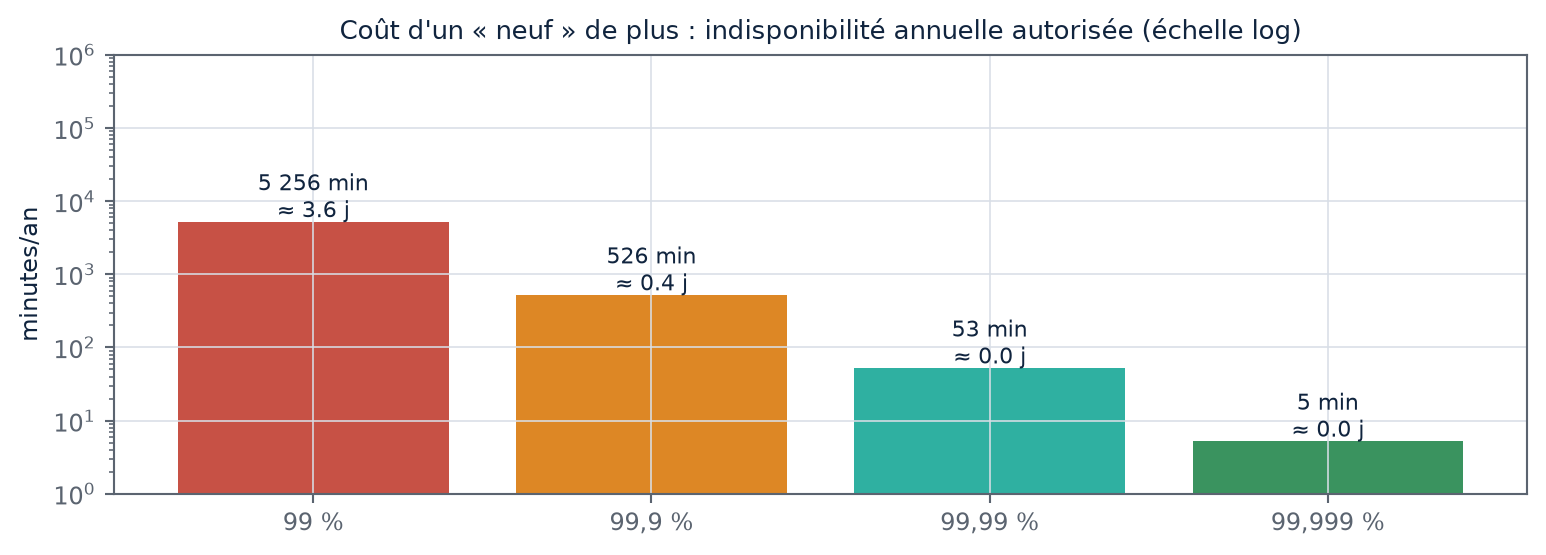
\includegraphics[width=0.88\textwidth]{f06_sla.png}
\end{center}
\begin{itemize}
\item Chaque 9 supplémentaire \textbf{divise le temps d'indisponibilité autorisé par 10} :
passer de 99,9 \% à 99,99 \% = passer de 8,8 h à 53 min d'arrêt \emph{annuel}.
\item Conséquence : à 99,999 \%, une panne de \textbf{30 min} consomme
5,7 \textbf{ans} de budget d'erreur. On ne « rattrape » pas une panne à ce niveau.
\end{itemize}
\end{frame}

\begin{frame}{Calculs de disponibilité : le rituel}
\begin{columns}[t]
\begin{column}{0.48\textwidth}
\begin{block}{Les deux formules}
\[
\text{Disponibilité} = \frac{\text{temps de service correct}}{\text{temps total}}
= 1 - \frac{\text{indisponibilité}}{\text{temps total}}
\]
\[
\text{MTBF} = \frac{\text{temps total de service}}{\text{nombre de pannes}}
\qquad
\text{MTTR} = \frac{\text{temps cumulé de réparation}}{\text{nombre de pannes}}
\]
\end{block}
\begin{ebox}[Exemple calculé sur NOSYS]
16 incidents $\times$ 8 serveurs = 16 blocs sur le mois, durées
35 et 50 min (0,58 h et 0,83 h). Indisponibilité cumulée du parc :
$8 \times (0{,}58 + 0{,}83) = 11{,}3$ h sur $8 \times 720$ h
$\Rightarrow$ disponibilité \textbf{99,80 \%}.
\end{ebox}
\end{column}
\begin{column}{0.48\textwidth}
\begin{wbox}[Conclusion à retenir]
Avec 2 incidents/serveur/mois, NOSYS \textbf{rate son SLA de 99,9 \%}
(99,80 \% atteint). Toute la mission ML des séances 3--4 se résume à :
\textbf{transformer ces 11,3 h de panne réactive en prévention}.
\end{wbox}
\begin{qbox}[Pour le prochain cours]
Si un prédictif détecte 70 \% des incidents 30 min à l'avance et que
l'équipe les évite, quelle devient la disponibilité ?
(faites le calcul --- réponse en séance 4.)
\end{qbox}
\end{column}
\end{columns}
\end{frame}

\begin{frame}{Quiz 2 --- les indicateurs (5 min)}
\begin{qbox}[3 questions]
\begin{enumerate}
\item Le p99 de latence est de 16 ms. Combien de requêtes sur 1 000 dépassent ce seuil ?\\
(a) 1 \quad (b) 10 \quad (c) 99
\item Un serveur a 6 pannes de 20 min sur l'année (8 760 h). MTTR = 20 min ;
MTBF $\approx$ ?\\
(a) 1 460 h \quad (b) 8 760 h \quad (c) 120 min
\item Pourquoi suivre le p99 plutôt que la moyenne ?\\
(a) le p99 est plus facile à calculer \quad (b) la moyenne masque la queue
de distribution où se trouvent les utilisateurs pénalisés \quad
(c) le p99 est exigé par le SLA uniquement
\end{enumerate}
\end{qbox}
\vspace{1mm}
\begin{solbox}[Réponses]
\textbf{1 : b} --- p99 = 99 \% en dessous, 1 \% au-dessus = 10 sur 1 000.
\quad
\textbf{2 : a} --- MTBF = 8 760 / 6 $\approx$ 1 460 h.
\quad
\textbf{3 : b} --- la moyenne est dominée par la masse de requêtes rapides.
\end{solbox}
\end{frame}

\begin{frame}{À retenir de la partie anatomie}
\begin{kbox}[Les 5 idées de cette section]
\begin{enumerate}
\item Une infrastructure est une \textbf{pile de couches} ; chaque couche émet
ses données --- et un symptôme applicatif a souvent sa cause deux couches plus bas.
\item Superviser la \textbf{distribution} des métriques (p99), pas la moyenne.
\item \textbf{SLI} = ce qu'on mesure ; \textbf{SLO} = l'objectif interne ;
\textbf{SLA} = le contrat. Ne jamais les confondre devant un client.
\item La disponibilité se \textbf{calcule} : 99,9 \% = 8,8 h/an ;
chaque 9 supplémentaire divise le budget par 10.
\item NOSYS est à \textbf{99,80 \%} : l'UE entière vise à remonter ce chiffre
par la prédiction et la prévention.
\end{enumerate}
\end{kbox}
\end{frame}

% =====================================================================
%  Seance 1 -- C. Le croisement AIOps (frames 25--33)
% =====================================================================
\section{Le croisement : pourquoi le ML pour les opérations}

\begin{frame}{AIOps : le problème que le seuil fixe ne résout pas}
\footnotesize%
\begin{columns}[t]
\begin{column}{0.52\textwidth}
\begin{block}{La supervision « classique » en une ligne}
\py{if cpu > 90: alerte()} \quad --- un seuil \textbf{constant}, écrit à la main.
\end{block}
\begin{ebox}[Testé sur les vraies données NOSYS]
Sur les 69 120 fenêtres du mois, le seuil 90 \% détecte
\textbf{136 fenêtres} --- et ce sont \textbf{exactement} les 136 fenêtres
d'incident (0 faux positif, 0 raté). Verdict honnête :
\textbf{ce mois-ci, le seuil fixe fonctionne}.
\end{ebox}
\begin{wbox}[Pourquoi on n'en reste pas là]
\begin{enumerate}
\item \textbf{Chance structurelle} : le trafic normal plafonne à 55 \% de CPU ---
le seuil à 90 \% ne peut pas être dépassé hors incident. Un mois de trafic
différent (campagne, sauvegarde massive) créerait des \textbf{faux positifs}.
\item \textbf{Aveugle aux dégradations lentes} : une fuite mémoire qui monte
de +0,5 \%/jour ne franchit jamais le seuil avant la panne.
\item \textbf{Ignorant du contexte} : le même niveau n'a pas le même sens à 3 h
et à 14 h (saisonnalité jour/nuit mesurée : 10,0 \% vs 30,2 \%).
\end{enumerate}
\end{wbox}
\end{column}
\begin{column}{0.44\textwidth}
\begin{center}
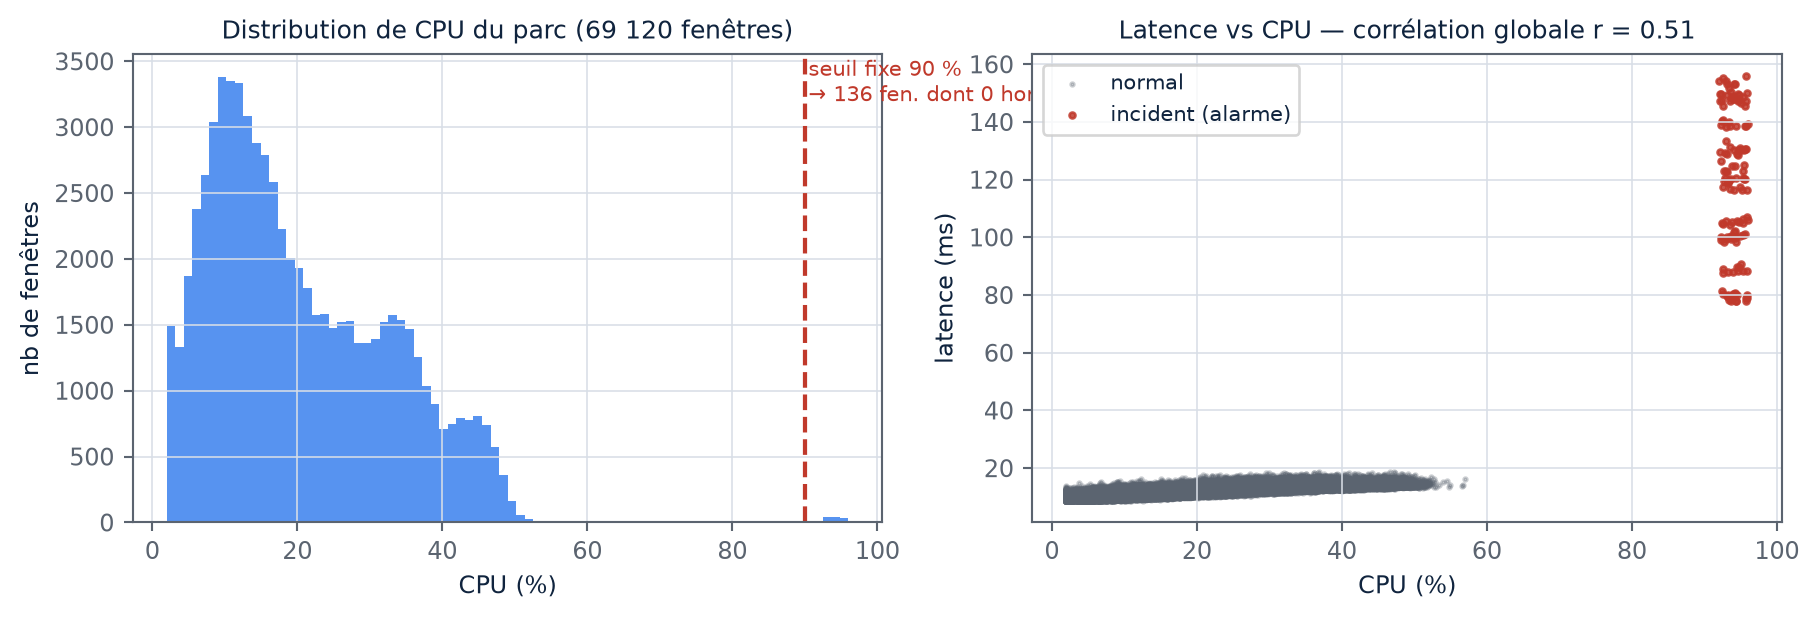
\includegraphics[width=\textwidth]{f05_seuil_vs_scatter.png}
\end{center}
\vspace{1mm}
\begin{kbox}[La bonne question]
Pas « au-dessus de quel seuil ? » mais
« \textbf{ce comportement est-il improbable} pour ce serveur, à cette heure,
dans cet état de charge ? ». C'est la définition d'un modèle.
\end{kbox}
\end{column}
\end{columns}
\end{frame}

\begin{frame}{La saisonnalité : le « normal » dépend de l'heure}
\begin{center}
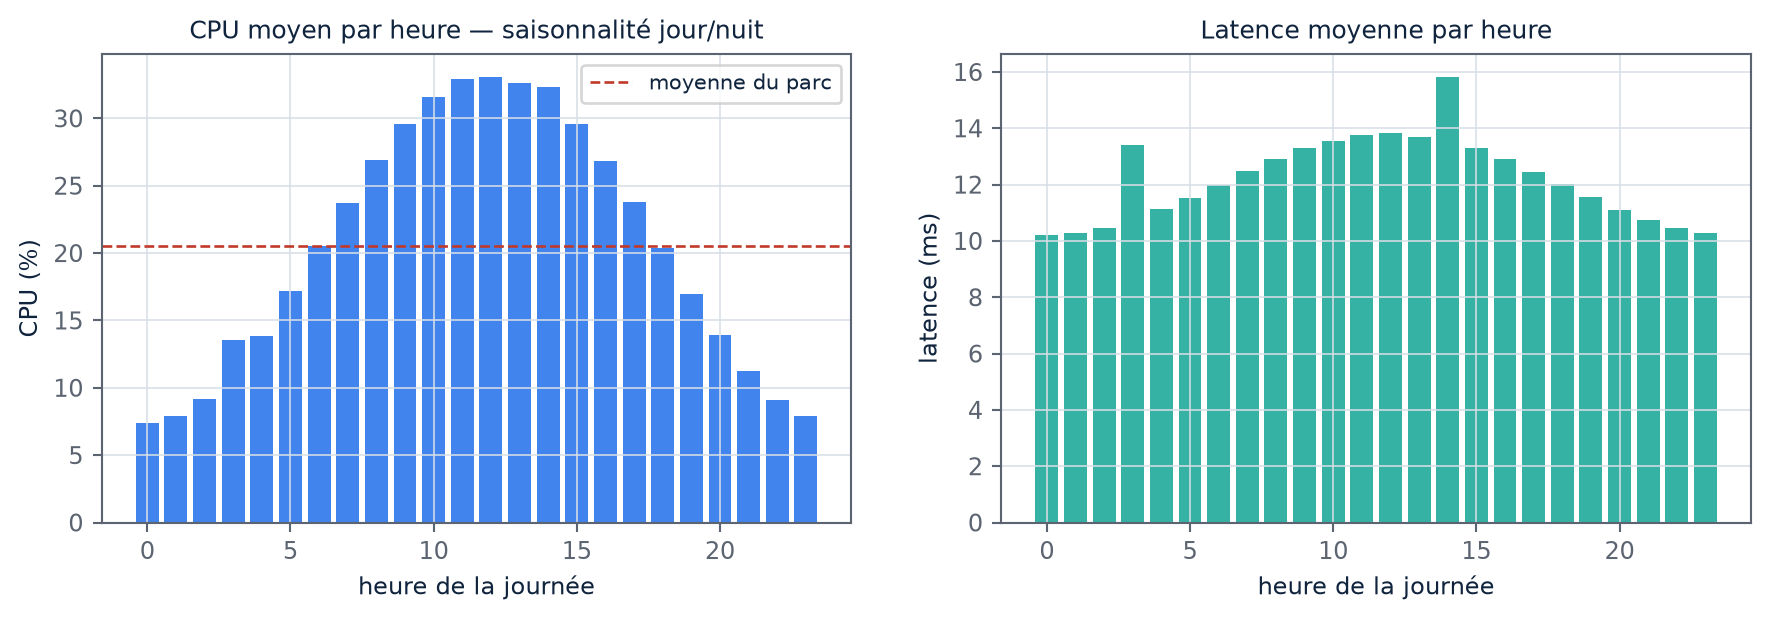
\includegraphics[width=0.92\textwidth]{f02_saisonnalite.png}
\end{center}
\begin{columns}[t]
\begin{column}{0.48\textwidth}
\begin{ebox}[Chiffres mesurés]
CPU moyen du parc : \textbf{30,2 \%} aux heures ouvrées (9 h--17 h),
\textbf{10,0 \%} la nuit (23 h--4 h) --- soit un \textbf{facteur 3}.
La latence suit le même profil.
\end{ebox}
\end{column}
\begin{column}{0.48\textwidth}
\begin{kbox}[Conséquence méthodologique]
Tout modèle sérieux encode le contexte temporel :
\textbf{heure, jour de semaine} (encodage cyclique, séance 2),
sinon il confond « 30 \% à 14 h » (normal) et « 30 \% à 3 h » (anomalie).
\end{kbox}
\end{column}
\end{columns}
\end{frame}

\begin{frame}{Zoom sur un incident : ce que le futur modèle verra}
\footnotesize%
\begin{center}
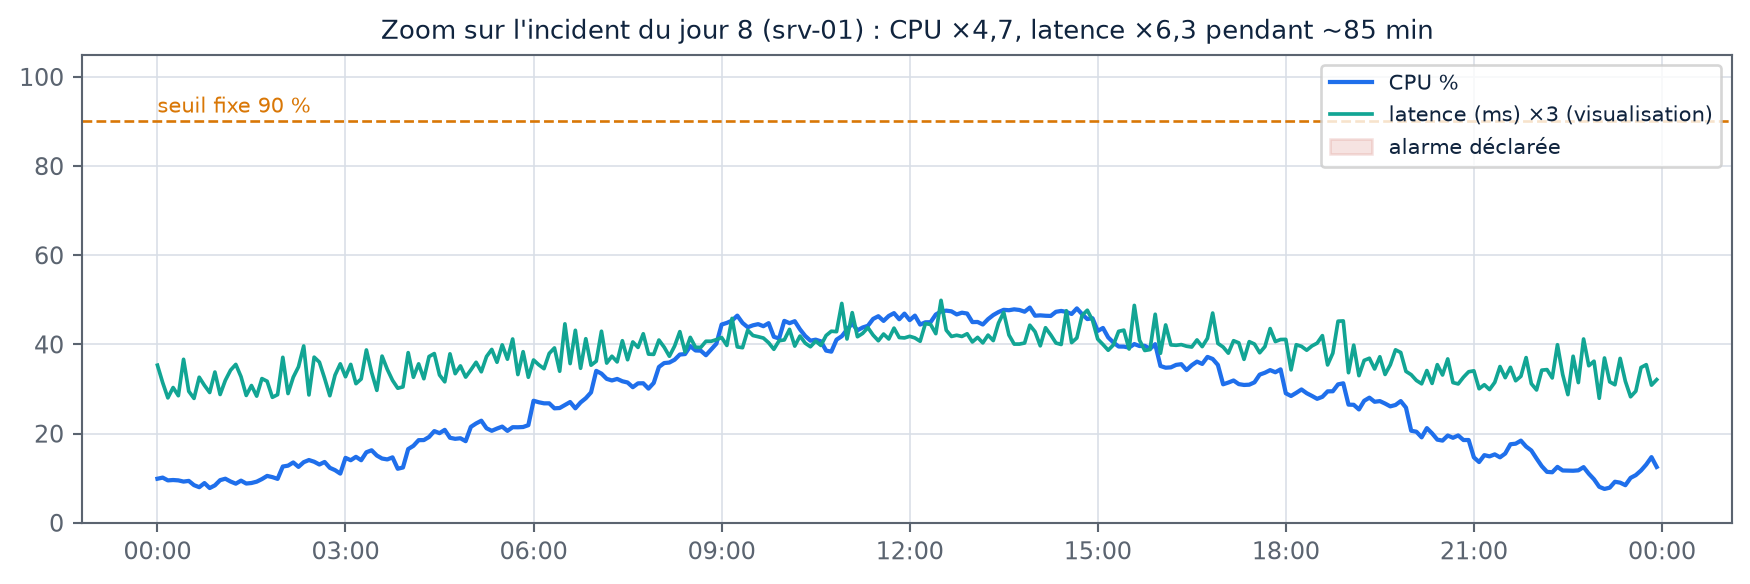
\includegraphics[width=0.94\textwidth]{f07_zoom_incident.png}
\end{center}
\begin{columns}[t]
\begin{column}{0.55\textwidth}
\begin{ebox}[Le jour 8 de srv-01 (incident réel du dossier)]
\begin{itemize}
\item Début \textbf{14 h 00}, durée \textbf{35 min} (7 fenêtres de 5 min).
\item CPU : de $\approx$ 30 \% à \textbf{95,7 \%} ($\times$ 3,2).
\item Latence : jusqu'à \textbf{156,1 ms} ($\times$ 12,8 vs p99 normal).
\item Perte de paquets multipliée par $\approx$ 5 pendant l'incident.
\end{itemize}
\end{ebox}
\end{column}
\begin{column}{0.41\textwidth}
\begin{kbox}[La question des séances 3--4]
Sur la \textbf{fenêtre de 14 h 00}, avant le pic : quels signaux précèdent
la montée ? Une \textbf{dérive} de RAM ? Une latence qui « pousse » ?
C'est exactement l'apprentissage supervisé de la cible
« incident dans les 30 min ».
\end{kbox}
\end{column}
\end{columns}
\end{frame}

\begin{frame}{La boucle AIOps complète}
\begin{center}
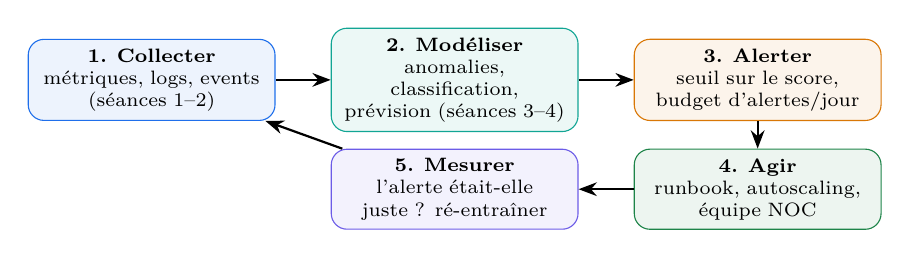
\begin{tikzpicture}[node distance=3.5mm and 7mm,
  box/.style={rectangle,rounded corners=2mm,draw,align=center,font=\scriptsize,
    minimum height=9mm,text width=2.9cm}]
\node[box,draw=byBlue,fill=byBlue!8]   (don) {\textbf{1. Collecter}\\métriques, logs, events\\(séances 1--2)};
\node[box,draw=byCyan,fill=byCyan!8,right=of don]  (mod) {\textbf{2. Modéliser}\\anomalies, classification,\\prévision (séances 3--4)};
\node[box,draw=byOrange,fill=byOrange!8,right=of mod] (ale) {\textbf{3. Alerter}\\seuil sur le score,\\budget d'alertes/jour};
\node[box,draw=byGreen,fill=byGreen!8,below=of ale] (act) {\textbf{4. Agir}\\runbook, autoscaling,\\équipe NOC};
\node[box,draw=byPurple,fill=byPurple!8,left=of act] (mes) {\textbf{5. Mesurer}\\l'alerte était-elle\\juste ? ré-entraîner};
\draw[-{Stealth},thick] (don) -- (mod);
\draw[-{Stealth},thick] (mod) -- (ale);
\draw[-{Stealth},thick] (ale) -- (act);
\draw[-{Stealth},thick] (act) -- (mes);
\draw[-{Stealth},thick] (mes) -- (don);
\end{tikzpicture}
\end{center}
\vspace{1mm}
\begin{itemize}
\item La boucle se \textbf{ferme} : chaque alerte jugée (juste/fausse) redevient
une \textbf{donnée d'entraînement} --- c'est ce qui distingue un AIOps vivant
d'un modèle figé.
\item Chaque séance de cette UE remplit une case de cette boucle ;
la séance 6 l'\textbf{industrialise} (API, retraining).
\end{itemize}
\end{frame}

\begin{frame}{Les quatre usages du ML en infrastructure --- la carte de l'UE}
\begin{center}
\small
\begin{tabular}{@{}p{3.4cm}p{5.2cm}p{2.2cm}p{3.4cm}@{}}
\toprule
\textbf{Usage} & \textbf{Question} & \textbf{Famille ML} & \textbf{Séance}\\
\midrule
Détection d'anomalies & Cette fenêtre est-elle improbable ? & Non supervisé & 3\\
\addlinespace[1pt]
Classification d'incident & Une panne dans les 30 min ? & Supervisé (classe rare) & 3--4\\
\addlinespace[1pt]
Prévision de charge & Quel trafic demain à 14 h ? & Séries temporelles & 4\\
\addlinespace[1pt]
Sécurité & Ces échecs d'auth forment-ils une attaque ? & Les deux & 5\\
\addlinespace[1pt]
Industrialisation & Le modèle survit-il en production ? & MLOps & 6\\
\bottomrule
\end{tabular}
\end{center}
\vspace{1mm}
\begin{kbox}[Ce que cette carte vous promet]
À la fin de l'UE, vous saurez \textbf{implémenter et déployer} chacun des
4 premiers usages sur des données réelles, et \textbf{expliquer} le cinquième.
\end{kbox}
\end{frame}

\begin{frame}{Quiz 3 --- AIOps (4 min)}
\footnotesize%
\begin{qbox}[3 questions]
\begin{enumerate}
\item Sur le mois NOSYS, le seuil fixe 90 \% a détecté 136/136 fenêtres d'incident.
Pourquoi ne pas s'arrêter là ?\\
(a) c'est de la chance structurelle : le trafic normal plafonne à 55 \% ;
dérives lentes et changement de trafic le contournent\\
(b) il faut un GPU\\ (c) le seuil était trop bas
\item La corrélation latence--CPU vaut 0,51 sur tout le mois mais
\textbf{0,80 hors incidents}. Interprétation la plus plausible ?\\
(a) la corrélation est instable \quad (b) les incidents créent des points
extrêmes qui écrasent la relation normale \quad (c) il y a une erreur de calcul
\item La boucle AIOps se distingue d'un simple modèle par\ldots\\
(a) son coût \quad (b) la mesure en boucle : chaque alerte jugée redevient
une donnée d'entraînement \quad (c) l'usage d'algorithmes plus récents
\end{enumerate}
\end{qbox}
\vspace{1mm}
\begin{solbox}[Réponses]
\textbf{1 : a} \quad \textbf{2 : b} --- c'est un effet classique des outliers ;
on le reverra (robustesse, séance 2). \quad \textbf{3 : b}
\end{solbox}
\end{frame}

% =====================================================================
%  Seance 1 -- D. Le dossier NOSYS + TP (frames 34--46)
% =====================================================================
\section{Le dossier NOSYS et les travaux pratiques}

\begin{frame}{Le dossier NOSYS : les données de la mission}
\begin{columns}[t]
\begin{column}{0.52\textwidth}
\begin{block}{\file{nosys\_metriques.csv} --- 69 120 lignes}
\begin{itemize}
\item \textbf{8 serveurs} (srv-01 \ldots srv-08) $\times$ \textbf{30 jours}
(01/09 -- 30/09/2026) $\times$ pas de \textbf{5 min}.
\item Colonnes : \py{horodatage}, \py{serveur}, \py{cpu\_pct}, \py{ram\_pct},
\py{latence\_ms}, \py{paquets\_perdus\_pct}, \py{temperature\_c}, \py{conso\_kwh},
\py{capacite\_cpu}, \py{alarme}.
\item \py{alarme} = 1 sur les fenêtres d'incident (déclarées a posteriori) :
\textbf{136 fenêtres} = 16 blocs de 35--50 min.
\end{itemize}
\end{block}
\begin{ebox}[Ce que le CSV ne contient PAS (volontairement)]
Aucune colonne « cause de l'incident » : en production, on découvre la cause
\emph{après}. Le TP demande de la retrouver \textbf{par l'analyse}.
\end{ebox}
\end{column}
\begin{column}{0.44\textwidth}
\begin{block}{\file{nosys\_logs.csv} --- 100 000 lignes}
Journaux d'authentification sur 7 jours : horodatage, machine, niveau,
utilisateur, message, \py{auth\_reussie}.
\begin{center}\small
\begin{tabular}{@{}lr@{}}
\toprule
Niveau & lignes\\
\midrule
INFO & 71 946\\
WARNING & 12 990\\
ERROR & 11 055\\
CRITICAL & 4 009\\
\bottomrule
\end{tabular}
\end{center}
\begin{center}\small
(séance 5 uniquement --- ne pas ouvrir aujourd'hui)
\end{center}
\end{block}
\end{column}
\end{columns}
\end{frame}

\begin{frame}{Vue d'ensemble : 8 serveurs, un mois, 2 incidents chacun}
\begin{center}
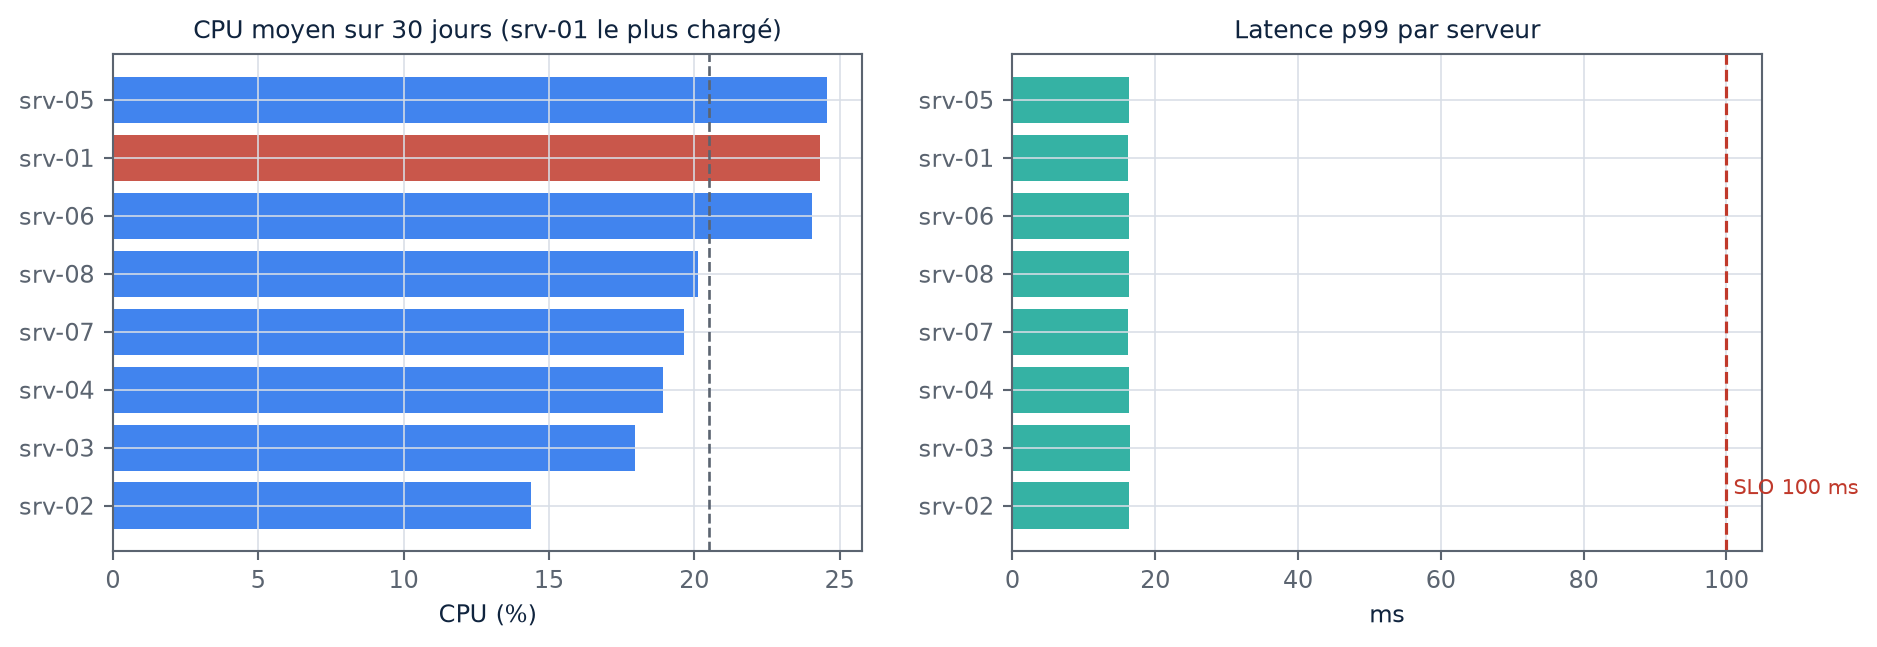
\includegraphics[width=0.95\textwidth]{f03_classement.png}
\end{center}
\begin{columns}[t]
\begin{column}{0.48\textwidth}
\begin{ebox}[Lecture à voix haute]
srv-01 et srv-05 portent les charges moyennes les plus élevées
(24,3 \% et 24,6 \%) ; tous les p99 restent sous le SLO de 100 ms
hors incidents (max 16,4 ms).
\end{ebox}
\end{column}
\begin{column}{0.48\textwidth}
\begin{kbox}[Le réflexe analyste]
Toujours commencer par \textbf{classement} + \textbf{comparaison à une
référence} (ici la moyenne du parc, 20,5 \%) avant tout modèle.
\end{kbox}
\end{column}
\end{columns}
\end{frame}

\begin{frame}{Quand les incidents arrivent-ils ?}
\begin{center}
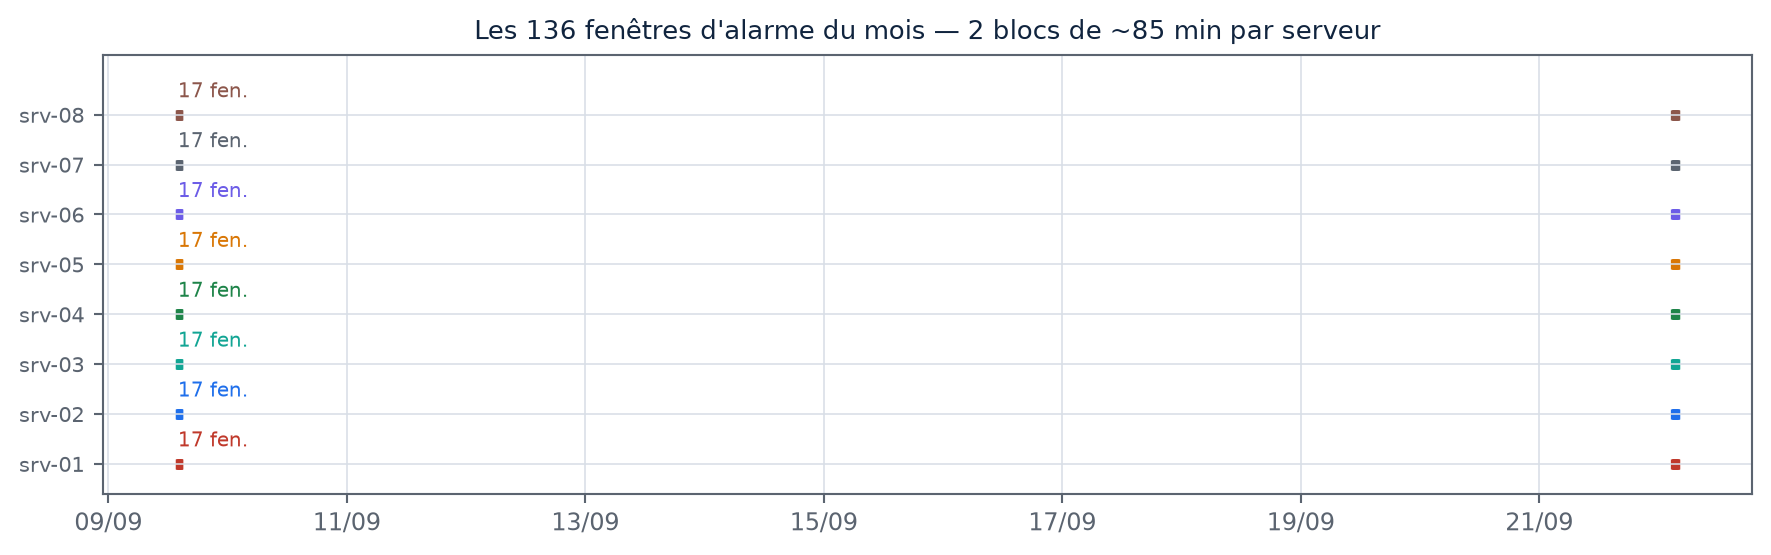
\includegraphics[width=0.95\textwidth]{f04_alarmes.png}
\end{center}
\begin{columns}[t]
\begin{column}{0.48\textwidth}
\begin{ebox}[Pattern remarquable]
Les 16 incidents se concentrent sur \textbf{2 créneaux} :
\textbf{9/09 à 14 h 00} (7 fenêtres, 35 min) et \textbf{22/09 à 3 h 00}
(10 fenêtres, 50 min) --- identiques sur les 8 serveurs.
\end{ebox}
\end{column}
\begin{column}{0.48\textwidth}
\begin{qbox}[Question d'ingénieur]
Une panne qui frappe \textbf{tous les serveurs en même temps} --- que suspecte-t-on
en priorité ?\\
(a) 8 disques défaillants simultanément \quad (b) une cause \textbf{partagée} :
batch de sauvegarde, mise à jour déployée, réseau \quad (c) le hasard
\end{qbox}
\vspace{1mm}
\begin{center}\small
Corrigé : (b) --- et c'est la première vraie question d'analyse que
vous poserez au TP (fenêtre commune = cause commune).
\end{center}
\end{column}
\end{columns}
\end{frame}

\begin{frame}{Premiers constats chiffrés (le niveau attendu du livrable)}
\begin{columns}[t]
\begin{column}{0.52\textwidth}
\begin{solbox}[Exemple de constats \textbf{correctement} rédigés]
\begin{enumerate}
\item Le parc est globalement sain : CPU moyen 20,5 \%,
p99 de latence \textbf{16,3 ms} pour un SLO à 100 ms
(marge $\times$ 6).
\item Mais la disponibilité calculée est \textbf{99,80 \%} $<$ SLA 99,9 \% :
11,3 h d'indisponibilité cumulée sur le mois.
\item Les 16 incidents suivent \textbf{2 créneaux communs} à tous les serveurs
(9/09 14 h, 22/09 3 h) : cause partagée probable (batch/déploiement),
pas 16 pannes matérielles indépendantes.
\item Corrélation latence--CPU \textbf{0,80} hors incidents : la charge
\emph{explique} la latence normale --- utile pour la prévision de la séance 4.
\item Consommation totale : \textbf{11 614 kWh}/mois ; srv-05 et srv-01
en tête (1 585 et 1 577 kWh).
\end{enumerate}
\end{solbox}
\end{column}
\begin{column}{0.44\textwidth}
\begin{wbox}[Le niveau \textbf{non} acceptable]
« Le CPU varie », « il y a des incidents », « les serveurs sont différents ».
Un constat sans \textbf{chiffre ni comparaison} ne valide rien.
\end{wbox}
\begin{kbox}[La règle du kit]
Un constat = un chiffre + une référence (moyenne, SLO, autre serveur)
+ une phrase d'interprétation.
\end{kbox}
\end{column}
\end{columns}
\end{frame}

\begin{frame}[fragile]{TP B1 --- charger et vérifier (30 min)}
\begin{codebox}[B1. Chargement et contrôles de base]
\begin{lstlisting}
import pandas as pd, numpy as np
import matplotlib.pyplot as plt

m = pd.read_csv("data/nosys_metriques.csv", parse_dates=["horodatage"])
print(m.shape)              # (69120, 10)
print(m["serveur"].unique())  # 8 serveurs
print(m["horodatage"].min(), "->", m["horodatage"].max())

# le pas d'echantillonnage est-il constant ?
print(m["horodatage"].diff().value_counts().head())
# -> attendu : 300s (5 min) partout, sauf le premier point (NaT)

# valeurs manquantes ?
print(m.isna().sum())
\end{lstlisting}
\end{codebox}
\begin{wbox}[Deux pièges classiques dès la première cellule]
\begin{enumerate}
\item Oublier \py{parse\_dates} : l'horodatage devient du texte,
et \py{.dt.hour} échoue plus loin.
\item Travailler dans un mauvais répertoire : donne le chemin complet
ou lance Jupyter depuis le dossier des données.
\end{enumerate}
\end{wbox}
\end{frame}

\begin{frame}{TP B2 --- inventaire de qualité (20 min)}
\begin{columns}[t]
\begin{column}{0.5\textwidth}
\begin{abox}[À produire]
\begin{enumerate}
\item Tableau : par colonne --- type, plages (min/max), nb de valeurs manquantes.
\item Vérifier que chaque serveur a bien \textbf{8 640 fenêtres} (30 j $\times$ 288/j).
\item Vérifier la cohérence : \py{0 <= cpu\_pct <= 100},
\py{ram\_pct} dans [0, 100], températures plausibles pour une salle
($>$ 20 °C ?).
\end{enumerate}
\end{abox}
\end{column}
\begin{column}{0.46\textwidth}
\begin{kbox}[Pourquoi ce rituel d'abord]
\begin{itemize}
\item Un \textbf{outlier de saisie} (CPU = 900) ruine moyenne, écart-type,
et tout modèle entraîné dessus.
\item Le nombre de fenêtres par serveur valide la \textbf{complétude} :
une fenêtre manquante est un trou invisible dans un graphe journalier mais
fatal à un rééchantillonnage.
\end{itemize}
\end{kbox}
\begin{ebox}[Réponse attendue sur NOSYS]
0 valeur manquante partout ; CPU max 96,0 \% ;
température max 42,7 °C : tout est plausible ---
vous pourrez le dire \textbf{avec la preuve}.
\end{ebox}
\end{column}
\end{columns}
\end{frame}

\begin{frame}[fragile]{TP B3 --- visualiser srv-01 sur 30 jours (30 min)}
\begin{codebox}[B3. Vue journalière + repérage des incidents]
\begin{lstlisting}
s1 = m[m["serveur"] == "srv-01"]
jour = (s1.set_index("horodatage")
          .drop(columns=["serveur"])
          .resample("D").mean())     # 30 lignes, une par jour

fig, ax = plt.subplots(3, 1, figsize=(11, 6), sharex=True)
ax[0].plot(jour.index, jour["cpu_pct"]);  ax[0].set_ylabel("CPU %")
ax[1].plot(jour.index, jour["latence_ms"]); ax[1].set_ylabel("latence ms")
ax[2].bar(jour.index, jour["alarme"]*4, width=0.7)  # fenetres x4 visible
ax[2].set_ylabel("alarmes (x4)")
plt.show()
\end{lstlisting}
\end{codebox}
\begin{abox}[Questions à répondre par le graphe]
\begin{enumerate}
\item Où sont les 2 incidents de srv-01 ? Quels jours, quelles heures ?
\item Le seuil fixe « alerte si CPU $>$ 90 \% » les aurait-il détectés ?
\item La latence monte-t-elle \textbf{en même temps} que le CPU ?
\end{enumerate}
\end{abox}
\end{frame}

\begin{frame}[fragile]{TP B4 --- statistiques par serveur (40 min)}
\footnotesize%
\begin{codebox}[B4. Le tableau de classement + les exercices]
\begin{lstlisting}
par_srv = (m.groupby("serveur")
             .agg(cpu_moy=("cpu_pct", "mean"),
                  cpu_max=("cpu_pct", "max"),
                  lat_p99=("latence_ms", lambda s: s.quantile(0.99)),
                  temp_max=("temperature_c", "max"),
                  alarmes=("alarme", "sum"),
                  conso_kwh_tot=("conso_kwh", lambda s: s.sum()*5/60),
                  capacite=("capacite_cpu", "first")))
par_srv.sort_values("cpu_moy", ascending=False)
\end{lstlisting}
\end{codebox}
\begin{columns}[t]
\begin{column}{0.48\textwidth}
\begin{abox}[Exercices]
\begin{enumerate}
\item Classer par CPU moyen ; surligner srv-01.
\item Ratio d'utilisation effective :
\py{cpu\_moy / (capacite*100)} --- quel serveur est le plus
« tassé » relativement à sa capacité ?
\item Consommation totale du parc sur le mois (kWh).
\end{enumerate}
\end{abox}
\end{column}
\begin{column}{0.48\textwidth}
\begin{ebox}[Réponses de contrôle]
CPU moyen : srv-05 24,6 \%, srv-01 24,3 \%, srv-02 14,4 \%.
Consommation totale : \textbf{11 614 kWh}.
Ratio le plus élevé : srv-01 (capacité 0,83 ---
le plus sollicité \emph{relativement} à ses moyens).
\end{ebox}
\begin{wbox}[Piège du lambda]
\py{lambda s: s.sum()*5/60} : ne pas oublier le pas de 5 min ---
sans lui, la consommation est divisée par 12.
\end{wbox}
\end{column}
\end{columns}
\end{frame}

\begin{frame}{TP B5 --- livrable : la fiche « état des lieux » (20 min + finition)}
\begin{columns}[t]
\begin{column}{0.52\textwidth}
\begin{abox}[Ce que vous rendez (1 page)]
\begin{enumerate}
\item \textbf{5 constats chiffrés} --- chacun : un chiffre, une référence,
une phrase d'interprétation (modèle : slide « premiers constats »).
\item \textbf{3 risques pour le SLA}, reliés aux données
(ex. : incidents synchrones entre serveurs ; CPU $\times$ 3,2 pendant
les incidents ; la corrélation latence--CPU 0,80 hors incidents
$\Rightarrow$ un pic de charge prévisible $\Rightarrow$ latence prévisible).
\item \textbf{1 recommandation} d'automatisation : quel problème des
séances à venir traiterait quel risque.
\end{enumerate}
\end{abox}
\end{column}
\begin{column}{0.44\textwidth}
\begin{kbox}[Barème indicatif (20 pts)]
\begin{itemize}
\item Constats chiffrés et corrects --- 10 pts
\item Risques reliés aux données --- 5 pts
\item Notebook exécutable, commenté, reproductible --- 5 pts
\end{itemize}
\end{kbox}
\begin{wbox}[Rappel reproductibilité]
Fixez la graine si vous simulez, citez le fichier de données,
et gardez les cellules \textbf{exécutables de haut en bas}
--- le correcteur relance votre notebook.
\end{wbox}
\end{column}
\end{columns}
\end{frame}

\begin{frame}{Les pièges du TP, récapitulés}
\begin{columns}[t]
\begin{column}{0.48\textwidth}
\begin{wbox}[Erreurs Python fréquentes]
\begin{itemize}
\item \py{read\_csv} sans \py{parse\_dates} $\Rightarrow$ pas de \py{.dt.hour}.
\item \py{resample("D").mean()} sur un DataFrame qui contient encore
la colonne \py{serveur} (texte) $\Rightarrow$ \py{TypeError}. Solution :
\py{.drop(columns=["serveur"])} avant.
\item Moyenner des percentiles : \py{p99 des moyennes} $\ne$ \py{p99}.
\item Boucle \py{for} sur 69 120 lignes : toujours \textbf{vectoriser}.
\end{itemize}
\end{wbox}
\end{column}
\begin{column}{0.48\textwidth}
\begin{wbox}[Erreurs d'analyse fréquentes]
\begin{itemize}
\item Conclure « pas d'anomalie » parce que le CPU moyen est bas :
les incidents sont \textbf{rares} (0,2 \% des fenêtres).
\item Confondre corrélation et causalité (CPU $\uparrow$ et latence $\uparrow$
peuvent partager une cause).
\item Rédiger des constats sans référence de comparaison.
\end{itemize}
\end{wbox}
\begin{ebox}[Si vous terminez en avance]
Représentez le \textbf{CPU par heure de la journée} pour srv-01
(\py{groupby(m["horodatage"].dt.hour)}) et vérifiez le facteur
jour/nuit $\times$ 3 annoncé en cours.
\end{ebox}
\end{column}
\end{columns}
\end{frame}

% =====================================================================
%  Seance 1 -- E. Synthese, quiz final, cloture (frames 47--50)
% =====================================================================
\section{Synthèse de la séance 1}

\begin{frame}{Quiz de synthèse --- 6 questions (10 min)}
\footnotesize%
\begin{qbox}[Répondez seul(e), puis correction collective]
\begin{enumerate}
\item Prévoir la consommation de la salle la semaine prochaine est :\\
(a) classification \quad (b) régression supervisée \quad (c) non supervisé
\item La disponibilité de NOSYS (16 incidents, durées 35/50 min, 8 serveurs, 30 j) :\\
(a) 99,99 \% \quad (b) 99,80 \% \quad (c) 99,50 \%
\item Un modèle classifieur donne 99,98 \% d'exactitude sur les incidents.\\
(a) c'est un excellent modèle \quad (b) la métrique est trompeuse : il
prédit peut-être jamais d'incident \quad (c) le modèle est parfait
\item Le p99 de latence du parc est 16,3 ms. Combien de requêtes sur
10 000 dépassent 16,3 ms ?\\
(a) 1 \quad (b) 100 \quad (c) 9 900
\item Un seuil fixe a tout détecté ce mois-ci. Le principal risque résiduel est :\\
(a) il consomme trop de CPU \quad (b) dérive lente et changement de trafic
le contournent \quad (c) les alarmes arrivent trop vite
\item La corrélation latence--CPU passe de 0,80 (hors incidents) à 0,51 (tout le mois).
Cela s'explique par :\\
(a) un bug \quad (b) les points d'incident, extrêmes, écrasent la relation normale
\quad (c) la corrélation n'existe pas
\end{enumerate}
\end{qbox}
\end{frame}

\begin{frame}{Corrigé du quiz de synthèse}
\begin{solbox}[Réponses justifiées]
\begin{enumerate}
\item \textbf{b} --- cible continue $\Rightarrow$ régression (séries temporelles, séance 4).
\item \textbf{b} --- indisponibilité $= 8 \times (0{,}58+0{,}83) = 11{,}3$ h ;
$1 - 11{,}3 / 5\,760 = 99{,}80$ \% (8 serveurs $\times$ 720 h).
\item \textbf{b} --- incidents $=$ 0,2 \% des fenêtres : « toujours non » atteint
99,8 \% sans aucun intérêt. Matrice de confusion obligatoire.
\item \textbf{b} --- 1 \% de 10 000 $=$ 100 requêtes lentes ; sur 10 M/jour,
100 000 requêtes concernées.
\item \textbf{b} --- démontré en cours : dérive lente $<$ 90 \% invisible,
et le « 0 faux positif » de ce mois tient au plafond de trafic à 55 \%.
\item \textbf{b} --- effet classique des valeurs extrêmes ; on apprendra à
robustifier (séance 2) et à modéliser \emph{hors} incidents d'abord.
\end{enumerate}
\end{solbox}
\end{frame}

\begin{frame}{Les 5 messages à emporter}
\begin{kbox}[Si vous ne retenez que ceci]
\begin{enumerate}
\item Le ML \textbf{apprend} le normal au lieu de le coder : c'est ce qui
détecte ce qu'aucun seuil écrit à la main ne peut couvrir.
\item Supervisez des \textbf{distributions} (p99), jamais des moyennes seules.
\item \textbf{SLI $\to$ SLO $\to$ SLA} : la chaîne mesure $\to$ objectif $\to$ contrat.
NOSYS est à 99,80 \% contre un SLA de 99,9 \% --- la mission est lancée.
\item Le \textbf{contexte temporel} fait partie du signal : 30 \% à 14 h $\ne$
30 \% à 3 h (facteur jour/nuit mesuré : 3).
\item Un constat d'analyse vaut par ses \textbf{chiffres et ses références} ---
c'est la règle de notation du TP.
\end{enumerate}
\end{kbox}
\end{frame}

\begin{frame}{Prochaine séance \& travail à faire}
\footnotesize%
\begin{columns}[t]
\begin{column}{0.52\textwidth}
\begin{ebox}[Séance 2 --- Données d'infrastructures et préparation]
\begin{itemize}
\item Où vivent les données : métriques (Prometheus, SNMP), journaux (syslog, ELK),
traces, events --- et leurs pièges (horloges, trous, granularités).
\item Préparation : rééchantillonnage, imputation, standardisation, encodage.
\item \textbf{Ingénierie de signaux} : fenêtres glissantes, p99 par fenêtre,
dérivées, encodage cyclique de l'heure --- le jour où « 3 h du matin »
devient une feature exploitable.
\end{itemize}
\end{ebox}
\end{column}
\begin{column}{0.44\textwidth}
\begin{abox}[Avant la séance 2]
\begin{enumerate}
\item Rendre le notebook du TP (fiche « état des lieux »).
\item (Facultatif) installer \py{great\_expectations} --- on le mentionnera.
\item Relire le calcul de disponibilité : la question « 70 \% des incidents
évités $\Rightarrow$ ? » attendue en séance 4 sera notée en TD.
\end{enumerate}
\end{abox}
\begin{center}\small
\textbf{Déroulé réalisé aujourd'hui :} 14h00 cours (A1--A4) · 16h15 TP (B1--B5) · 18h15 fin.
\end{center}
\end{column}
\end{columns}
\end{frame}

% =====================================================================
%  Seance 2 -- A. garde, plan, ou vivent les donnees (frames 1--9)
% =====================================================================
\section{Séance 2 --- Données d'infrastructures et préparation}
\chapterslide{Séance 2}{Données d'infrastructures et préparation des données}
{4 h --- 2 h cours / 2 h TP --- Partie 2 du syllabus EPD-GIT-5534}
{\textbf{Objectifs :} connaître les sources de données d'une infrastructure et
leurs pièges (granularité, horloges) $\bullet$ maîtriser le nettoyage :
doublons, valeurs manquantes, valeurs aberrantes $\bullet$ construire des
\textbf{signaux} (fenêtres, p99, encodage cyclique) $\bullet$ produire le
\textbf{jeu de données supervisé} du dossier (étiquette « incident $\le$ 30 min »).}

\begin{frame}{Plan de la séance (4 h)}
\begin{columns}[t]
\begin{column}{0.48\textwidth}
\begin{kbox}[Cours magistral --- 2 h]
\begin{enumerate}
\item \textbf{Où vivent les données} (40 min) : métriques, journaux, événements,
traces --- granularités et horloges.
\item \textbf{Préparer les données} (60 min) : doublons, manquants, aberrants,
rééchantillonnage.
\item \textbf{Ingénierie de signaux} (20 min) : fenêtres, p99, encodage cyclique,
dérive de capteur.
\end{enumerate}
\end{kbox}
\end{column}
\begin{column}{0.48\textwidth}
\begin{ebox}[Travaux pratiques --- 2 h]
\textbf{« Du brut au dataset supervisé »} sur \file{nosys\_metriques\_brutes.csv} :
\begin{enumerate}
\item B1 --- audit des défauts (30 min)
\item B2 --- nettoyage : doublons, NaN, aberrants (35 min)
\item B3 --- signaux : fenêtres, p99, encodage cyclique (30 min)
\item B4 --- étiquette « incident $\le$ 30 min » (35 min)
\item B5 --- livrable : \file{nosys\_features.csv} + dictionnaire (10 min)
\end{enumerate}
\end{ebox}
\end{column}
\end{columns}
\vspace{1mm}
\begin{center}\small
Nouveau fichier du dossier : la \textbf{collecte brute} avec ses défauts réels ---
le TP part du brut, pas du propre.
\end{center}
\end{frame}

\begin{frame}{Où vivent les données d'une infrastructure ?}
\begin{center}
\small
\begin{tabular}{@{}p{2.3cm}p{4.6cm}p{2.6cm}p{3.6cm}@{}}
\toprule
\textbf{Source} & \textbf{Contenu} & \textbf{Granularité} & \textbf{Exemple}\\
\midrule
\textbf{Métriques} & séries temporelles numériques & 10 s -- 5 min &
Prometheus, SNMP, agents (notre \py{cpu\_pct})\\
\addlinespace[1pt]
\textbf{Journaux} & événements textuels datés & à l'événement &
syslog, ELK (\file{nosys\_logs.csv})\\
\addlinespace[1pt]
\textbf{Événements} & alertes, déploiements, incidents & ponctuel &
PagerDuty, webhooks (\py{alarme})\\
\addlinespace[1pt]
\textbf{Traces} & parcours d'une requête entre services & par requête &
OpenTelemetry, Jaeger\\
\addlinespace[1pt]
\textbf{Tickets} & interventions humaines, causes & ponctuel &
ServiceNow, Jira --- la « vérité terrain »\\
\bottomrule
\end{tabular}
\end{center}
\vspace{1mm}
\begin{kbox}[La règle d'or du ML applicatif]
Un bon modèle d'infrastructure \textbf{joint} plusieurs sources :
métriques (le symptôme) + événements (le contexte) + tickets (la cause).
La séance 2 construit cette jointure.
\end{kbox}
\end{frame}

\begin{frame}{Granularité et horloges : les pièges silencieux}
\begin{columns}[t]
\begin{column}{0.5\textwidth}
\begin{block}{Granularité hétérogène}
Dans notre collecte brute, \textbf{srv-07 relève toutes les 15 min} alors
que les 7 autres relèvent toutes les 5 min (config d'agent différente).
\begin{itemize}
\item Une jointure naïve sur l'horodatage \textbf{perd} les données srv-07.
\item Il faut \textbf{rééchantillonner} vers une grille commune (séance : f09).
\end{itemize}
\end{block}
\begin{block}{Horloges}
\begin{itemize}
\item Tout serveur n'a pas la même heure (dérive NTP, fuseaux).
\item Règle : collecter en \textbf{UTC}, convertir à l'affichage.
\item Un décalage de 2 min entre deux sources détruit une jointure à la minute.
\end{itemize}
\end{block}
\end{column}
\begin{column}{0.46\textwidth}
\begin{wbox}[Le défaut que personne ne voit]
Pas de valeur manquante affichée, pas d'erreur : \textbf{juste moins de
points}. Un compte de lignes par serveur révèle la granularité :
srv-07 a 2\,880 points au lieu de 8\,640.
\end{wbox}
\begin{qbox}[Question]
Vous jointez métriques (5 min) et logs (à l'événement). Pourquoi une
jointure \py{merge} exacte échoue presque toujours ?\\
(a) les logs sont trop nombreux \quad (b) les horodatages ne coïncident
jamais exactement --- il faut \textbf{as-of join} / fenêtres \quad
(c) il faut du SQL
\end{qbox}
\end{column}
\end{columns}
\end{frame}

\begin{frame}{Le fichier du TP : une collecte « comme en production »}
\footnotesize%
\begin{columns}[t]
\begin{column}{0.52\textwidth}
\begin{ebox}[\file{nosys\_metriques\_brutes.csv} --- 63 521 lignes]
Les défauts semés (graine 5534, script \file{make\_nosys\_s2.py}) :
\begin{itemize}
\item \textbf{200 lignes dupliquées} (ré-tentative réseau).
\item \textbf{5 508 valeurs manquantes} (1,73 \% des cellules numériques) ---
capteur flottant.
\item \textbf{12 valeurs aberrantes} : température à \textbf{1 575 °C},
CPU à \textbf{350 \%} --- pic de capteur, pas d'incident.
\item \textbf{6 trous} de 15 à 40 min (agent redémarré).
\item \textbf{srv-07 en granularité 15 min}.
\item \textbf{srv-06 : capteur de température qui dérive}.
\end{itemize}
\end{ebox}
\end{column}
\begin{column}{0.44\textwidth}
\begin{center}
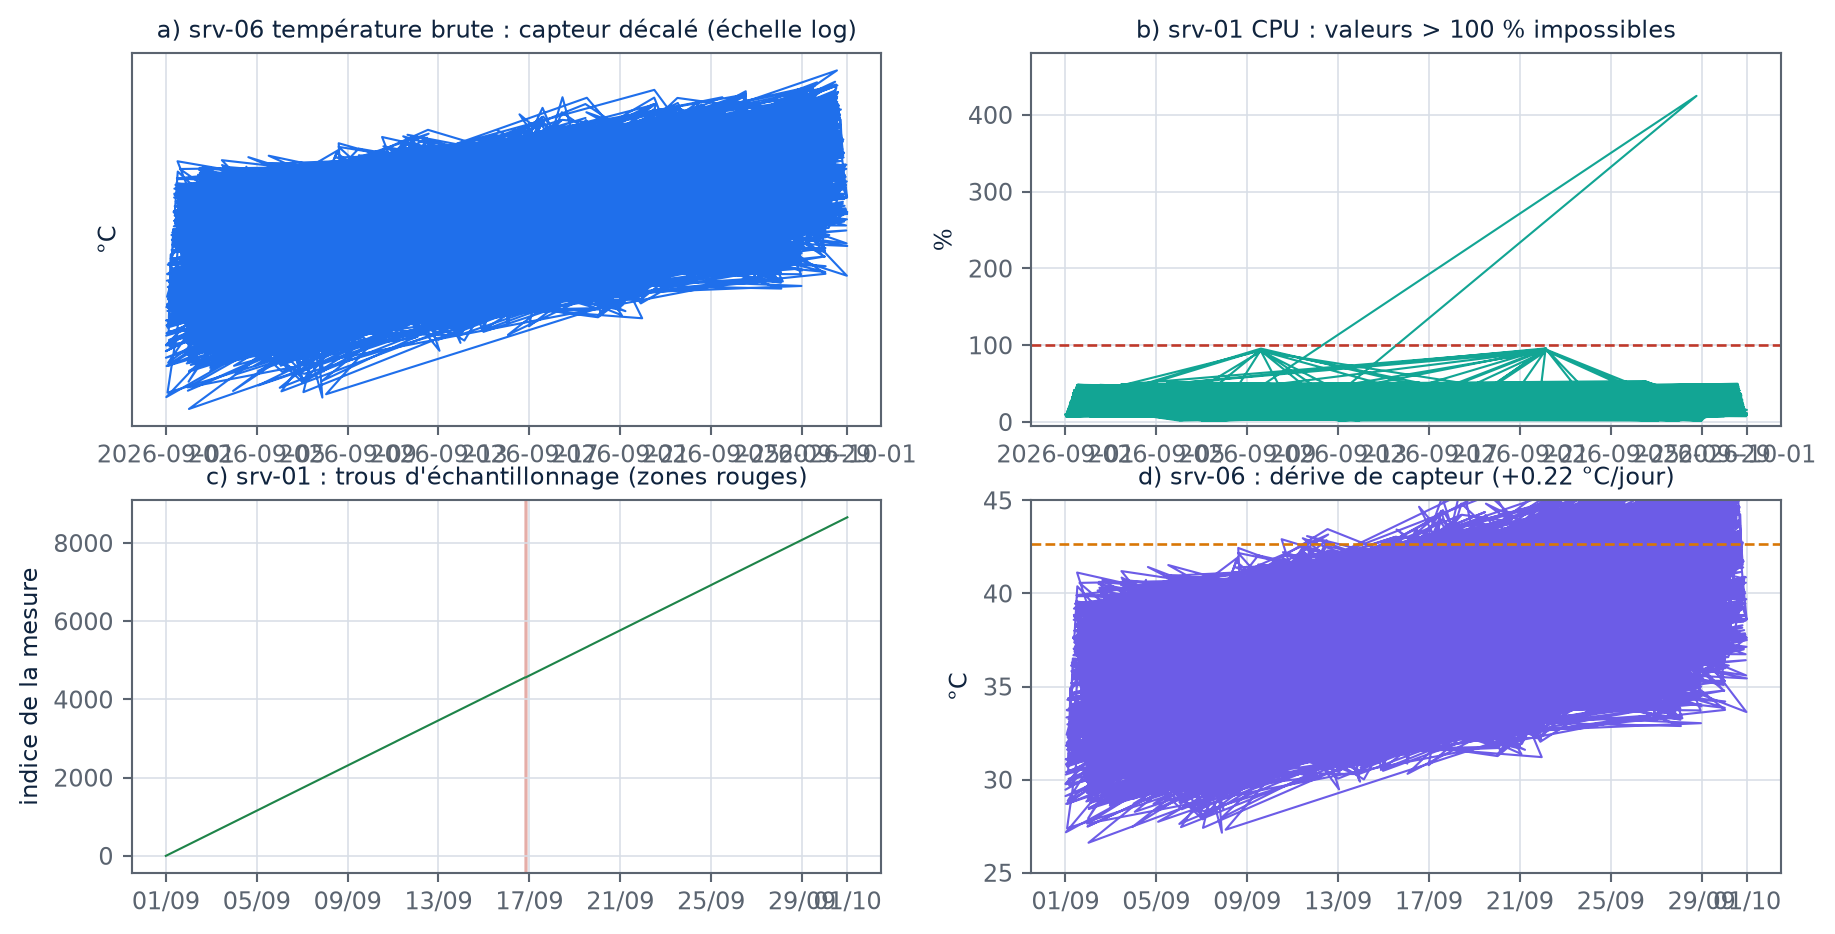
\includegraphics[width=\textwidth]{f08_defauts.png}
\end{center}
\end{column}
\end{columns}
\end{frame}

\begin{frame}{Quiz 1 --- les sources (5 min)}
\begin{qbox}[3 questions]
\begin{enumerate}
\item Quelle source donne la \textbf{cause} d'un incident (et pas seulement le symptôme) ?\\
(a) les métriques \quad (b) les tickets et journaux d'intervention \quad
(c) les traces
\item srv-07 relève toutes les 15 min. Sur un mois, il produit :\\
(a) 8 640 points \quad (b) 2 880 points \quad (c) 28 800 points
\item Le pire défaut d'une jointure métriques/logs naïve est :\\
(a) elle est lente \quad (b) les horodatages ne coïncident jamais exactement
$\Rightarrow$ presque tout est perdu \quad (c) elle crée des doublons
\end{enumerate}
\end{qbox}
\vspace{1mm}
\begin{solbox}[Réponses]
\textbf{1 : b} \quad \textbf{2 : b} (288/jour $\times$ 30) \quad \textbf{3 : b} ---
d'où les jointures par \textbf{fenêtre} (as-of / \py{merge\_asof}).
\end{solbox}
\end{frame}

% =====================================================================
%  Seance 2 -- B. Preparer les donnees (frames 10--18)
% =====================================================================
\section{Préparer les données : doublons, manquants, aberrants}

\begin{frame}[fragile]{Étape 0 : trier et dédoublonner}
\footnotesize%
\begin{codebox}[Le rituel des 3 premières lignes de tout pipeline]
\begin{lstlisting}
b = pd.read_csv("data/nosys_metriques_brutes.csv", parse_dates=["horodatage"])

# 1. trier : la collecte arrive dans le desordre
b = b.sort_values(["serveur", "horodatage"]).reset_index(drop=True)

# 2. dedoublonner : 200 lignes exactement identiques (re-tentative reseau)
print(b.duplicated().sum())        # -> 200
b = b.drop_duplicates()

# 3. verifier la completude : nb de points attendus par serveur
b.groupby("serveur").size()
\end{lstlisting}
\end{codebox}
\begin{columns}[t]
\begin{column}{0.48\textwidth}
\begin{ebox}[Ce que révèle l'étape 3 sur le fichier brut]
7 serveurs à $\approx$ 8 600 points, \textbf{srv-07 à 2 880} : la
granularité 15 min se voit immédiatement dans le compte.
\end{ebox}
\end{column}
\begin{column}{0.48\textwidth}
\begin{wbox}[Pourquoi trier AVANT tout le reste]
Diff, fenêtres glissantes et interpolation supposent l'ordre
temporel. Sur un fichier « brûlé » (ordre mélangé), une moyenne
mobile calculée avant le tri est \textbf{mathématiquement fausse}
--- sans qu'aucune erreur ne soit levée.
\end{wbox}
\end{column}
\end{columns}
\end{frame}

\begin{frame}{Valeurs manquantes : trois mécanismes, trois réponses}
\begin{center}
\footnotesize
\begin{tabular}{@{}p{2.4cm}p{4.8cm}p{5.0cm}@{}}
\toprule
\textbf{Mécanisme} & \textbf{Ce que c'est} & \textbf{Réponse adaptée}\\
\midrule
\textbf{MCAR} & manquant \emph{au hasard} (capteur flottant) &
imputation simple acceptable\\
\addlinespace[1pt]
\textbf{MAR} & manquant \emph{lié à une autre variable observée} &
modèle d'imputation (KNN, régression)\\
\addlinespace[1pt]
\textbf{MNAR} & manquant \emph{pour une raison liée à sa valeur}
(le CPU à 100 \% fait planter l'agent !) &
ne jamais imputer aveuglément : documenter, traiter le trou comme signal\\
\bottomrule
\end{tabular}
\end{center}
\vspace{1mm}
\begin{columns}[t]
\begin{column}{0.52\textwidth}
\begin{ebox}[Dans le fichier brut NOSYS]
\textbf{5 508} cellules manquantes (1,73 \% des cellules numériques),
réparties uniformément sur les 5 colonnes (1 072 à 1 123 chacune) :
profil \textbf{MCAR} --- capteurs flottants. Imputation justifiée,
\textbf{après} vérification du profil.
\end{ebox}
\end{column}
\begin{column}{0.44\textwidth}
\begin{kbox}[Le test à faire systématiquement]
Comparer le taux de manquants \textbf{pendant les incidents} et
\textbf{hors incidents}. Si les manquants se concentrent pendant les
incidents $\Rightarrow$ MNAR : l'absence de donnée \emph{est} une information.
\end{kbox}
\end{column}
\end{columns}
\end{frame}

\begin{frame}{Imputer : forward-fill contre interpolation}
\begin{center}
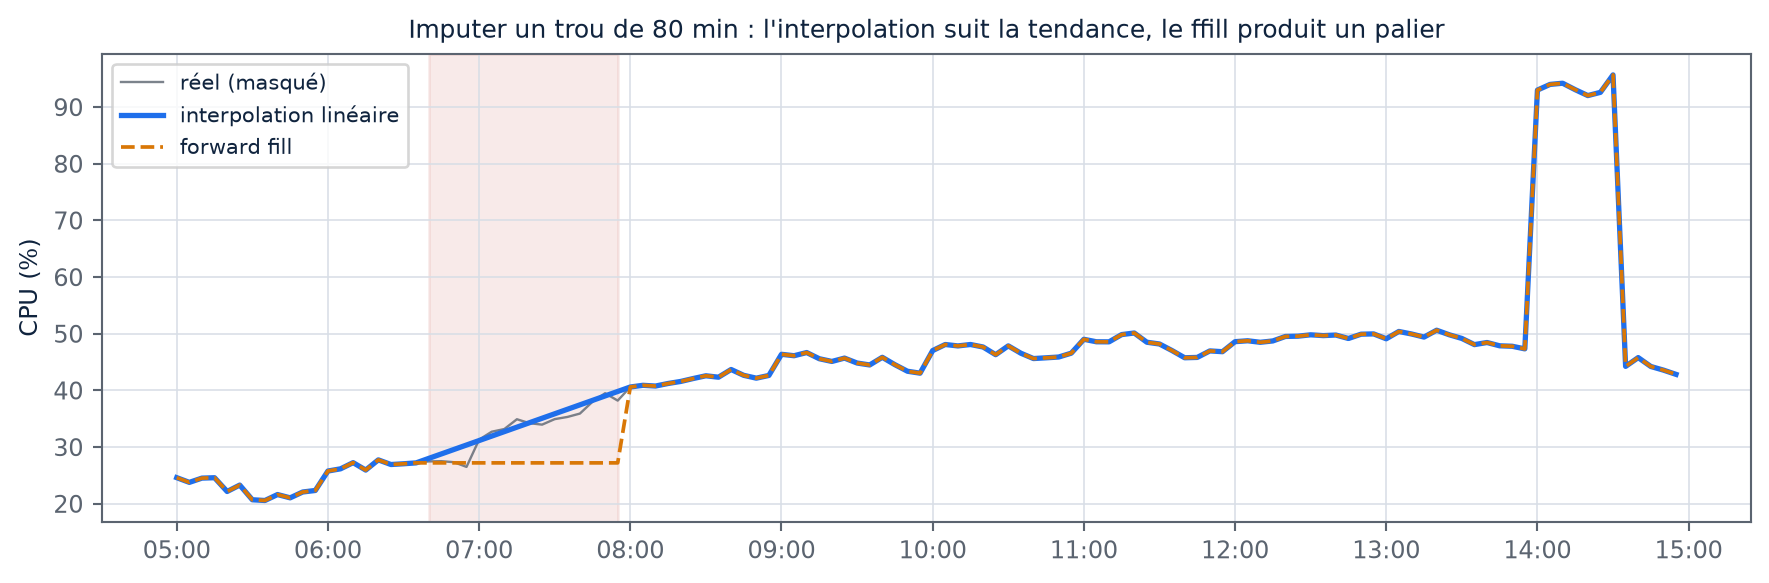
\includegraphics[width=0.94\textwidth]{f13_imputation.png}
\end{center}
\begin{columns}[t]
\begin{column}{0.52\textwidth}
\begin{ebox}[Erreur mesurée sur CPU (600 points masqués, srv-01)]
\begin{itemize}
\item \textbf{Forward-fill} (recopier la dernière valeur) :
erreur absolue moyenne \textbf{1,018} points de CPU.
\item \textbf{Interpolation linéaire} :
\textbf{0,743} --- 27 \% mieux, car le signal évolue en tendance.
\end{itemize}
\end{ebox}
\end{column}
\begin{column}{0.44\textwidth}
\begin{wbox}[La règle du pas]
Jamais d'imputation au-delà d'1--2 pas. Au-delà (trou de 40 min),
interpoler \textbf{invente} des données : mieux vaut marquer le trou
et l'exclure des fenêtres d'entraînement.
\end{wbox}
\end{column}
\end{columns}
\end{frame}

\begin{frame}{Valeurs aberrantes : z-score et IQR en pratique}
\footnotesize%
\begin{center}
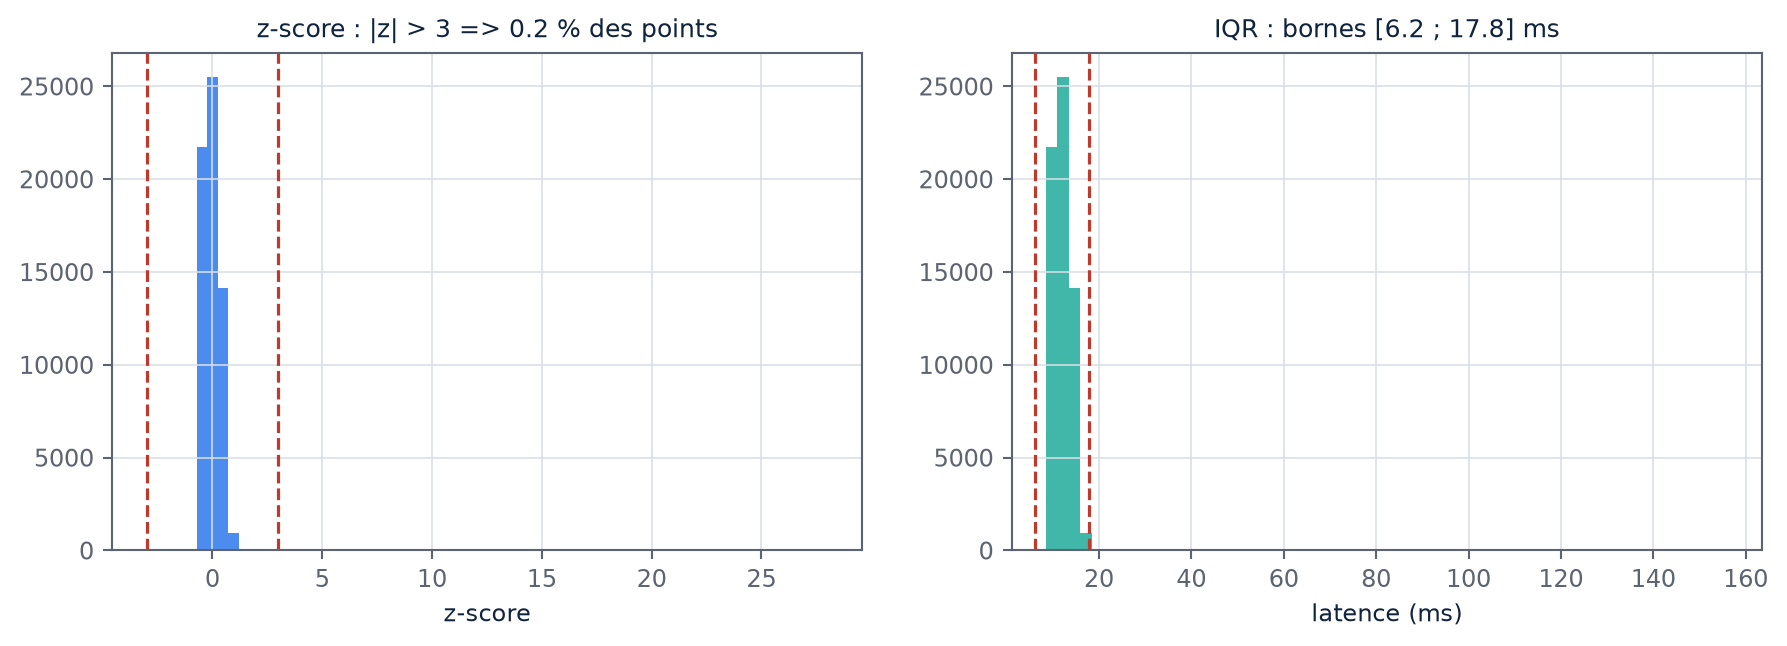
\includegraphics[width=0.92\textwidth,height=3.9cm,keepaspectratio]{f12_outliers.png}
\end{center}
\begin{columns}[t]
\scriptsize
\begin{column}{0.5\textwidth}
\begin{ebox}[Sur la latence du fichier brut]
Après exclusion des 12 pics capteur (latence $>$ 400 ms) :
\begin{itemize}
\item bornes IQR : \py{[Q1 - 1.5*IQR ; Q3 + 1.5*IQR]} ;
\item bornes z-score : moyenne $\pm$ 3 écart-types.
\item Les deux se recouvrent ; l'IQR reste \textbf{robuste} si la loi
est asymétrique.
\end{itemize}
\end{ebox}
\end{column}
\begin{column}{0.46\textwidth}
\begin{wbox}[Le défaut à ne JAMAIS faire]
Supprimer tout ce qui dépasse ! Ici, \textbf{les incidents sont des
valeurs extrêmes légitimes} (CPU 96 \%).
\begin{itemize}
\item Distinguer \textbf{erreur de mesure} (1 575 °C, CPU 350 \% :
impossible) et \textbf{événement réel} (CPU 96 \%).
\item Règle métier d'abord : bornes physiques, puis statistiques.
\end{itemize}
\end{wbox}
\end{column}
\end{columns}
\end{frame}

\begin{frame}[fragile]{Rééchantillonner : du pas irrégulier à la grille commune}
\begin{codebox}[Normaliser la granularité (srv-07 en 15 min $\to$ 5 min)]
\begin{lstlisting}
def normaliser(g):                      # g = un serveur
    g = g.set_index("horodatage").drop(columns=["serveur"])
    # grille reguliere de 5 min sur la plage du serveur
    grille = pd.date_range(g.index.min(), g.index.max(), freq="5min")
    return g.reindex(grille)            # les trous deviennent des NaN

b = b.groupby("serveur", group_keys=False).apply(normaliser)
\end{lstlisting}
\end{codebox}
\begin{columns}[t]
\begin{column}{0.5\textwidth}
\begin{center}
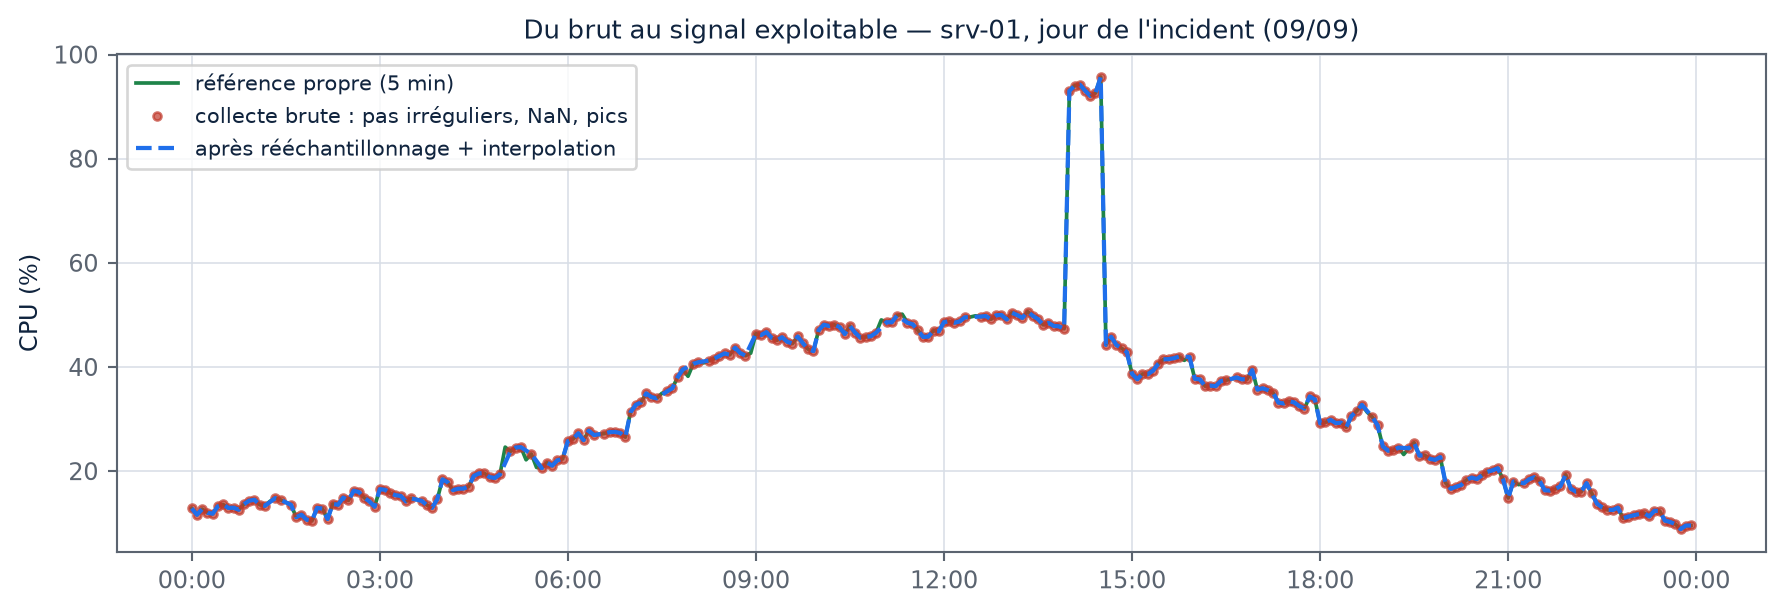
\includegraphics[width=\textwidth]{f09_reechantillonnage.png}
\end{center}
\end{column}
\begin{column}{0.46\textwidth}
\begin{kbox}[Ce que fait \py{reindex}]
Il crée la grille 5 min \textbf{explicite} : les trous (agent redémarré)
apparaissent comme \py{NaN} au lieu de disparaître silencieusement ---
on peut alors les compter, les tracer, les imputer ou les exclure
en connaissance de cause.
\end{kbox}
\end{column}
\end{columns}
\end{frame}

\begin{frame}{Quiz 2 --- préparation (5 min)}
\begin{qbox}[3 questions]
\begin{enumerate}
\item 5 508 manquants uniformément répartis sur les colonnes : quel mécanisme ?\\
(a) MNAR \quad (b) MAR \quad (c) MCAR
\item Un CPU affiché à 350 \%. Que fait-on ?\\
(a) on l'impute \quad (b) c'est une erreur de mesure (physiquement impossible)
$\Rightarrow$ on la corrige en NaN puis on impute \quad (c) on le garde, c'est
un incident
\item Pourquoi l'IQR est-il souvent préféré au z-score sur des métriques d'infra ?\\
(a) il est plus rapide \quad (b) il est robuste aux distributions
asymétriques (latence, queues longues) \quad (c) il détecte plus d'outliers
\end{enumerate}
\end{qbox}
\vspace{1mm}
\begin{solbox}[Réponses]
\textbf{1 : c} \quad \textbf{2 : b} --- CPU $>$ 100 \% n'existe pas ;
CPU 96 \% pendant un incident est, lui, légitime. \quad \textbf{3 : b}
\end{solbox}
\end{frame}

\begin{frame}{À retenir de la préparation}
\begin{kbox}[Les 5 règles du pipeline de préparation]
\begin{enumerate}
\item \textbf{Trier} par (serveur, temps) avant toute fenêtre ou interpolation.
\item \textbf{Dédoublonner} puis \textbf{compter} : la granularité se voit
dans les comptes (srv-07 : 2 880 points).
\item \textbf{Réindexer} sur une grille explicite : les trous deviennent
des NaN \emph{visibles}, jamais des silences.
\item Classer les manquants (\textbf{MCAR/MAR/MNAR}) avant de choisir
l'imputation --- et ne jamais imputer au-delà d'1--2 pas.
\item Distinguer \textbf{erreur de mesure} (impossible physiquement)
et \textbf{événement réel} : les incidents SONT des valeurs extrêmes légitimes.
\end{enumerate}
\end{kbox}
\end{frame}

% =====================================================================
%  Seance 2 -- C. Ingenierie de signaux (frames 19--27)
% =====================================================================
\section{Ingénierie de signaux : rendre les métriques apprenables}

\begin{frame}{Pourquoi des signaux ? Le modèle ne lit pas 69 120 lignes}
\begin{block}{Du point au signal}
Un modèle supervisé apprend sur des \textbf{unités d'observation} :
pour nous, une \textbf{fenêtre} (serveur $\times$ 10 min) décrite par
des \textbf{variables calculées} :
\begin{itemize}
\item niveau : CPU moyen, RAM moyenne sur la fenêtre ;
\item dispersion : écart-type, min/max, amplitude ;
\item distribution : \textbf{p99} de latence sur la fenêtre ;
\item dynamique : \textbf{dérivée} (le CPU monte-t-il ?), écart à la
saisonnalité horaire ;
\item contexte : heure encodée \textbf{cycliquement}, jour de semaine.
\end{itemize}
\end{block}
\begin{kbox}[C'est là que se gagne la prédiction]
La plupart des modèles de détection de panne perdent contre un bon
\textbf{feature engineering} : les variables contiennent la physique
du système, pas seulement les mesures brutes.
\end{kbox}
\end{frame}

\begin{frame}{Moyennes mobiles : extraire la tendance sans tuer les incidents}
\begin{center}
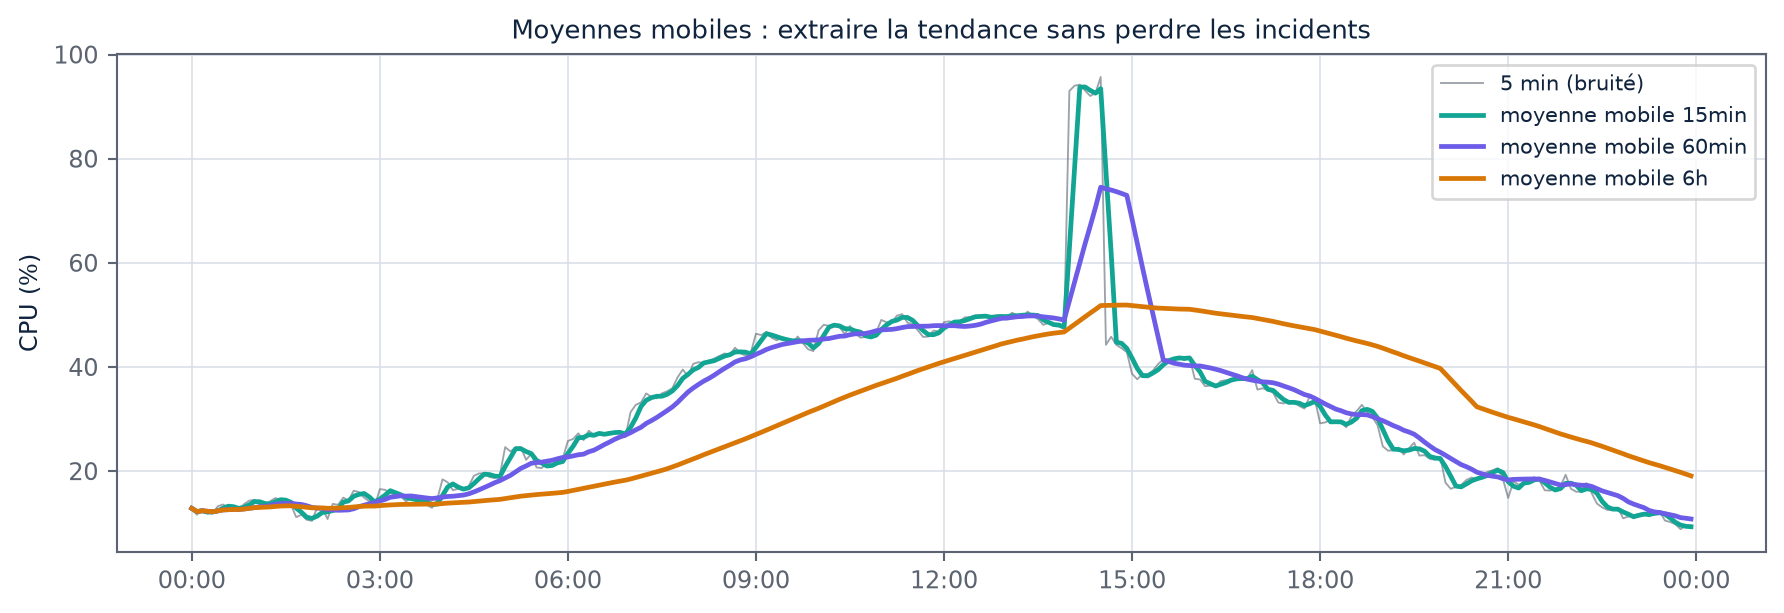
\includegraphics[width=0.94\textwidth]{f10_moyennes_mobiles.png}
\end{center}
\begin{columns}[t]
\begin{column}{0.5\textwidth}
\begin{ebox}[Lecture sur le jour de l'incident]
\begin{itemize}
\item 15 min : lisse le bruit, \textbf{garde} le pic de 14 h.
\item 60 min : donne la tendance, arrondit le pic.
\item 6 h : montre la saisonnalité jour/nuit, l'incident a disparu.
\end{itemize}
\end{ebox}
\end{column}
\begin{column}{0.46\textwidth}
\begin{kbox}[La règle de la fenêtre]
Choisir la fenêtre par rapport à ce qu'on veut prédire :
étiquette « incident $\le$ 30 min » $\Rightarrow$ signaux sur
\textbf{5 à 30 min}, jamais 6 h (l'information serait diluée).
\end{kbox}
\end{column}
\end{columns}
\end{frame}

\begin{frame}[fragile]{p99 par fenêtre : la variable qui voit la queue}
\begin{columns}[t]
\begin{column}{0.52\textwidth}
\begin{block}{Moyenne contre p99, par fenêtre de 10 min}
\begin{itemize}
\item La \textbf{moyenne} de latence est stable ($\approx$ 12 ms) --- même
pendant les prémices d'un incident.
\item Le \textbf{p99} par fenêtre explose \textbf{avant} que la moyenne ne
bouge : les requêtes lentes arrivent d'abord.
\item C'est pourquoi les SLO sont écrits en p99 (séance 1) --- et c'est
pourquoi nos features le seront aussi.
\end{itemize}
\end{block}
\begin{codebox}[En une ligne]
\begin{lstlisting}
f10 = (b.set_index("horodatage")
        .groupby("serveur")["latence_ms"]
        .resample("10min")
        .agg(lat_moy="mean", lat_p99=lambda s: s.quantile(0.99)))
\end{lstlisting}
\end{codebox}
\end{column}
\begin{column}{0.44\textwidth}
\begin{wbox}[Le piège du petit échantillon]
Sur une fenêtre de 10 min, il n'y a que \textbf{2 points} de métriques.
Le « p99 » de 2 points est presque le maximum --- c'est acceptable
(comme signal), mais il faut le \textbf{documenter} dans le dictionnaire
des variables : un p99 sur n=2 n'est pas un p99 statistique.
\end{wbox}
\begin{ebox}[Choix du pas du TP]
Métriques à 5 min $\Rightarrow$ fenêtre de \textbf{10 min} (2 points,
moyenne + max), étiquette regardant \textbf{30 min} en avant.
\end{ebox}
\end{column}
\end{columns}
\end{frame}

\begin{frame}[fragile]{Encodage cyclique : pourquoi 23 h et 0 h sont voisines}
\footnotesize%
\begin{center}
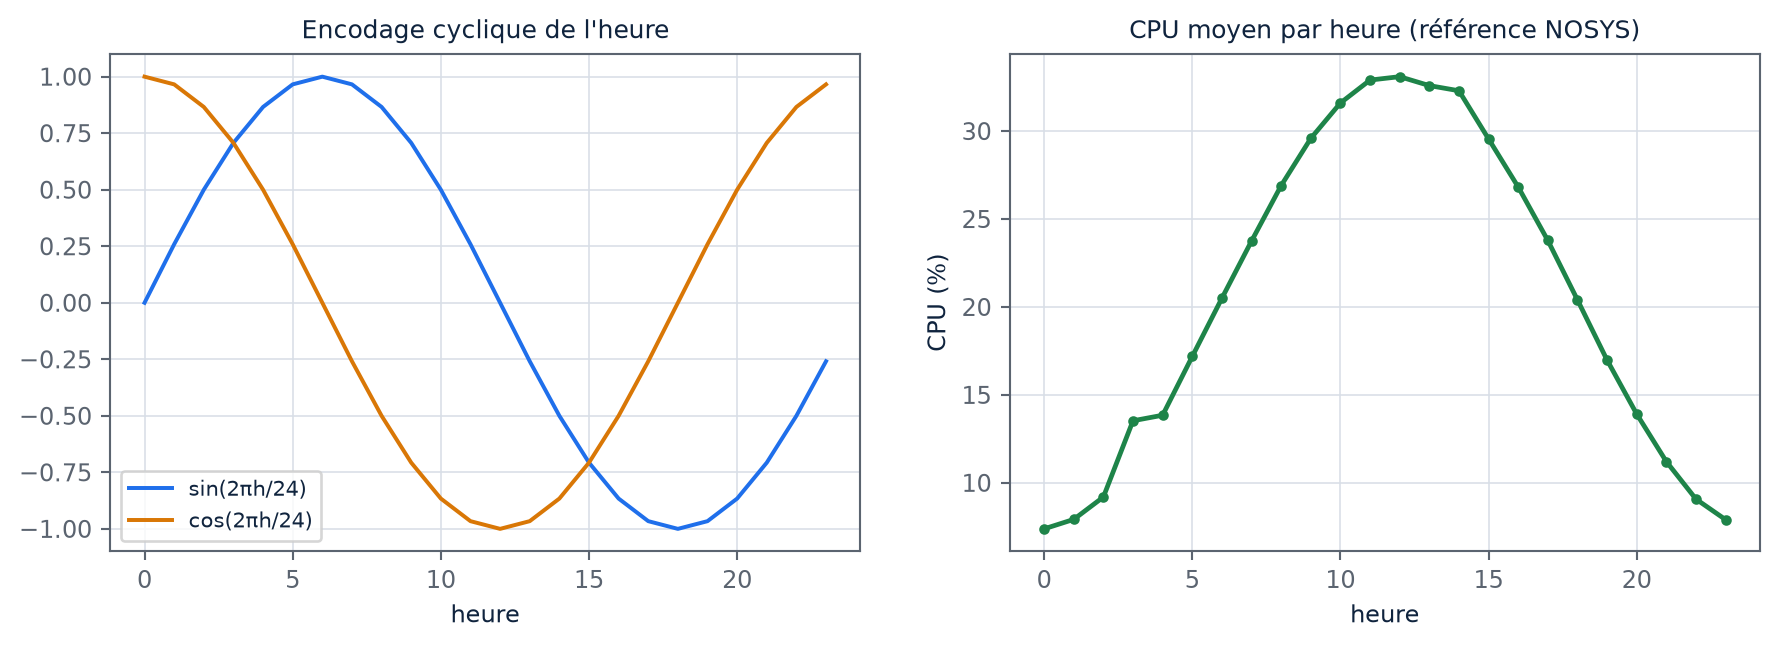
\includegraphics[width=0.80\textwidth]{f11_cyclique.png}
\end{center}
\begin{columns}[t]
\begin{column}{0.5\textwidth}
\begin{block}{Le problème de l'heure brute}
L'heure 23 et l'heure 0 sont \textbf{voisines} dans le réel
(1 h d'écart) mais \textbf{distantes de 23} dans la colonne brute.
Toute frontière cyclique (minuit, dimanche/lundi, décembre/janvier)
crée cette fausse discontinuité.
\end{block}
\begin{codebox}[La solution standard]
\begin{lstlisting}
h = b.index.hour
b["h_sin"] = np.sin(2*np.pi*h/24)
b["h_cos"] = np.cos(2*np.pi*h/24)
\end{lstlisting}
\end{codebox}
\end{column}
\begin{column}{0.46\textwidth}
\begin{kbox}[Pourquoi deux variables]
Un seul sinus replierait 6 h et 18 h sur la même valeur.
Le couple (sin, cos) place l'heure \textbf{sur un cercle} :
distance euclidienne = distance réelle entre heures.
Même traitement pour le \textbf{jour de semaine} (période 7)
et le \textbf{mois} (période 12).
\end{kbox}
\end{column}
\end{columns}
\end{frame}

\begin{frame}{La dérive de capteur : un défaut invisible aux seuils}
\footnotesize%
\begin{columns}[t]
\begin{column}{0.5\textwidth}
\begin{block}{Le cas srv-06}
Régression linéaire de la température sur le temps :
\begin{itemize}
\item pente mesurée : \textbf{+0,222 °C/jour} (fichier brut) ;
\item pente de référence (données propres) : $\approx$ 0.
\end{itemize}
Sur un mois : $+6{,}7$ °C --- sous aucun seuil, mais si la dérive
continue, la salle surchauffe \textbf{dans 2 mois}.
\end{block}
\begin{ebox}[Comment le détecter automatiquement]
Régression par fenêtre glissante (7 jours) : une pente
significativement $\ne$ 0 sur une métrique \emph{censée stationnaire}
= alerte de dérive. C'est un modèle \textbf{très simple qui remplace
un seuil impossible à écrire}.
\end{ebox}
\end{column}
\begin{column}{0.46\textwidth}
\begin{wbox}[Pourquoi les seuils ratent les dérives]
Un seuil alerte sur la \textbf{valeur absolue}. La dérive est un
problème de \textbf{tendance} : chaque valeur prise isolément est
normale, c'est leur \emph{enchaînement} qui ne l'est pas.
\end{wbox}
\begin{kbox}[Vocabulaire]
Ce test s'appelle \textbf{stationnarité} : une métrique de supervision
saine est stationnaire (moyenne et variance stables). On le formalisera
avec les séries temporelles (séance 4).
\end{kbox}
\end{column}
\end{columns}
\end{frame}

\begin{frame}{Standardiser : mettre toutes les échelles à égalité}
\footnotesize%
\begin{center}
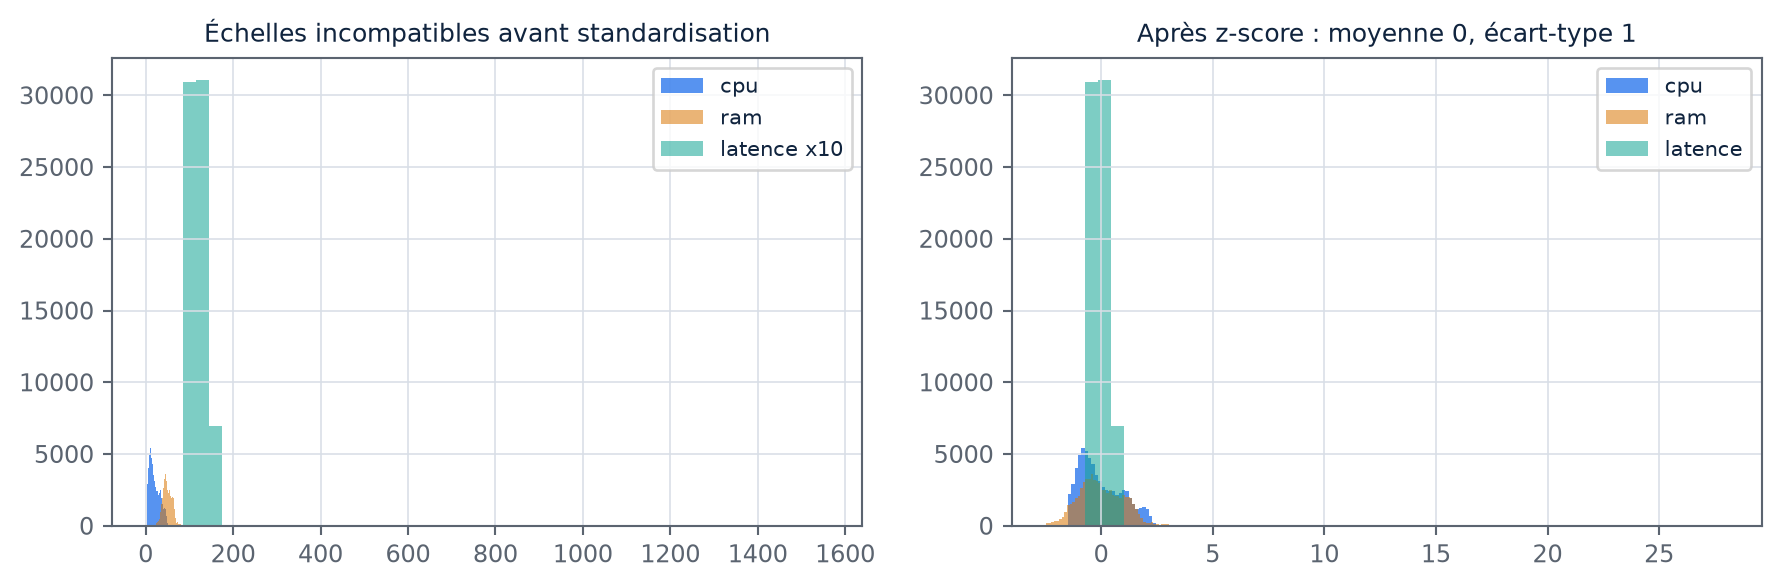
\includegraphics[width=0.94\textwidth]{f14_standardisation.png}
\end{center}
\begin{columns}[t]
\begin{column}{0.52\textwidth}
\begin{block}{Pourquoi c'est indispensable}
\begin{itemize}
\item CPU $\approx$ 20, RAM $\approx$ 50, latence $\approx$ 12 :
sans standardisation, un modèle à distances (k-NN, SVM) ou à
pénalité (ridge) est \textbf{dominé par la variable d'échelle la plus grande}.
\item $z = (x - \bar{x}) / \sigma$ : moyenne 0, écart-type 1.
\end{itemize}
\end{block}
\end{column}
\begin{column}{0.44\textwidth}
\begin{wbox}[Standardiser APRÈS le train/test split]
La moyenne et l'écart-type doivent être calculés \textbf{sur le train
seulement}, puis appliqués au test --- sinon on fait fuiter
l'information du futur. Avec les fenêtres temporelles de notre TP :
standardiser sur les 24 premiers jours, appliquer aux 6 derniers.
\end{wbox}
\end{column}
\end{columns}
\end{frame}

\begin{frame}{Quiz 3 --- signaux (5 min)}
\begin{qbox}[3 questions]
\begin{enumerate}
\item L'étiquette est « incident dans les 30 min ». La fenêtre de calcul
des signaux la mieux adaptée est :\\
(a) 6 h \quad (b) 24 h \quad (c) 5 à 30 min
\item Pourquoi encoder l'heure avec (sin, cos) plutôt qu'un nombre 0--23 ?\\
(a) c'est plus compact \quad (b) minuit sépare 23 h et 0 h alors qu'elles
sont voisines --- le cercle corrige \quad (c) les arbres l'exigent
\item La pente de température de srv-06 est +0,222 °C/jour. Le seuil
« alerte si T $>$ 45 °C » la détecte :\\
(a) immédiatement \quad (b) seulement quand la salle surchauffera ---
le seuil ne voit pas la \textbf{tendance} \quad (c) jamais
\end{enumerate}
\end{qbox}
\vspace{1mm}
\begin{solbox}[Réponses]
\textbf{1 : c} \quad \textbf{2 : b} \quad \textbf{3 : b} --- d'où la
régression glissante comme détecteur de dérive.
\end{solbox}
\end{frame}

% =====================================================================
%  Seance 2 -- D. TP du brut au dataset supervise + synthese
% =====================================================================
\section{TP « Du brut au dataset supervisé » et synthèse}

\begin{frame}{Le TP : objectif final, un jeu de données supervisé}
\footnotesize%
\begin{columns}[t]
\begin{column}{0.52\textwidth}
\begin{kbox}[Ce que vous produisez à 18 h]
\begin{center}
\file{nosys\_features.csv}\\[1mm]
une ligne = (serveur, fenêtre de 10 min)\\[1mm]
\begin{tabular}{@{}l@{}}
\toprule
variables de niveau : cpu\_moy, ram\_moy\ldots\\
dispersion : cpu\_max, cpu\_amplitude\\
distribution : lat\_p99\\
dynamique : cpu\_delta (dérivée)\\
contexte : h\_sin, h\_cos, jour\_sem\\
\textbf{cible : incident\_30min} $\in \{0,1\}$\\
\bottomrule
\end{tabular}
\end{center}
\end{kbox}
\begin{ebox}[Chiffres attendus]
\textbf{34 560} fenêtres (8 serveurs $\times$ 4 320), dont
\textbf{120 positives} (\textbf{0,35 \%}) --- une classe \emph{très} rare,
c'est exactement ce que la séance 3 apprendra à traiter.
\end{ebox}
\end{column}
\begin{column}{0.44\textwidth}
\begin{center}
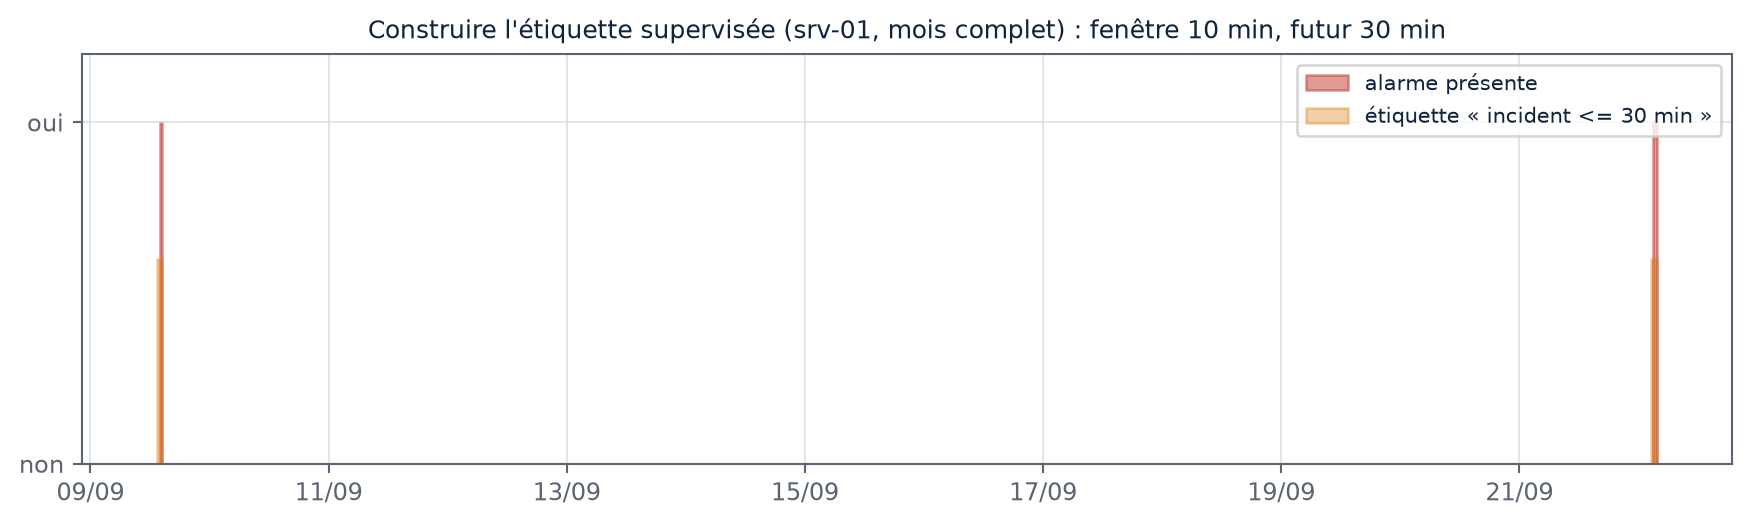
\includegraphics[width=\textwidth]{f15_etiquette.png}
\end{center}
\vspace{1mm}
\begin{wbox}[La règle anti-fuite]
Le calcul de \py{incident\_30min} utilise \textbf{uniquement} la colonne
\py{alarme} du futur. Les variables de signaux, elles, utilisent
\textbf{uniquement le passé} de la fenêtre. Mélanger les deux
$=$ tricher, et le modèle de la séance 3 paraîtra magique
en validation, nul en production.
\end{wbox}
\end{column}
\end{columns}
\end{frame}

\begin{frame}[fragile]{TP B1 --- audit des défauts (30 min)}
\begin{codebox}[B1. Compter, ne pas réparer encore]
\begin{lstlisting}
b = pd.read_csv("data/nosys_metriques_brutes.csv",
                parse_dates=["horodatage"])
b = b.sort_values(["serveur", "horodatage"]).reset_index(drop=True)

print("doublons :", b.duplicated().sum())          # 200
print("NaN par colonne :")
print(b[["cpu_pct","ram_pct","latence_ms",
         "paquets_perdus_pct","temperature_c"]].isna().sum())
print("valeurs impossibles :")
print("cpu > 100 :", (b["cpu_pct"] > 100).sum())        # 4
print("temp > 80 :", (b["temperature_c"] > 80).sum())   # 5
print("points par serveur :")
print(b.groupby("serveur").size())                 # srv-07 a 2880
\end{lstlisting}
\end{codebox}
\begin{abox}[Livrable B1]
Un tableau d'audit : \textbf{chaque défaut, son volume, son hypothèse de cause}
(doublon réseau, capteur flottant, pic capteur, redémarrage d'agent,
config de granularité, dérive). \textbf{Avant de réparer, on explique.}
\end{abox}
\end{frame}

\begin{frame}[fragile]{TP B2 --- nettoyage (35 min)}
\footnotesize%
\begin{codebox}[B2. Réparer dans le bon ordre]
\begin{lstlisting}
# 1. dedoublonner
b = b.drop_duplicates()

# 2. erreurs physiquement impossibles -> NaN (pas de suppression !)
b.loc[b["cpu_pct"] > 100, "cpu_pct"] = np.nan
b.loc[b["temperature_c"] > 80, "temperature_c"] = np.nan

# 3. grille explicite 5 min par serveur (les trous -> NaN visibles)
def sur_grille(g):
    g = g.set_index("horodatage").drop(columns=["serveur"])
    return g.reindex(pd.date_range(g.index.min(), g.index.max(),
                                   freq="5min"))
b = b.groupby("serveur", group_keys=False).apply(sur_grille)

# 4. imputation courte (<= 2 pas), tendance-compatible
b = b.interpolate(limit=2, limit_direction="both")
\end{lstlisting}
\end{codebox}
\begin{columns}[t]
\begin{column}{0.48\textwidth}
\begin{wbox}[Pourquoi « NaN » et pas « suppression »]
Supprimer une ligne d'incident suspecte, c'est supprimer
\textbf{l'exemple le plus précieux} du dataset. On neutralise
l'erreur de mesure, on garde l'observation.
\end{wbox}
\end{column}
\begin{column}{0.48\textwidth}
\begin{ebox}[Contrôle de sortie B2]
Après B2 : 0 doublon, 0 CPU $>$ 100, 0 NaN résiduels
(interpolation a couvert les trous courts), 8 serveurs
sur la même grille --- srv-07 inclus.
\end{ebox}
\end{column}
\end{columns}
\end{frame}

\begin{frame}[fragile]{TP B3 --- construire les signaux (30 min)}
\begin{codebox}[B3. Fenêtre de 10 min, par serveur]
\begin{lstlisting}
f = (b.reset_index().set_index("horodatage")
      .groupby("serveur")
      .resample("10min")
      .agg(cpu_moy=("cpu_pct", "mean"),
           cpu_max=("cpu_pct", "max"),
           ram_moy=("ram_pct", "mean"),
           lat_moy=("latence_ms", "mean"),
           lat_p99=("latence_ms", lambda s: s.quantile(0.99)),
           perte_moy=("paquets_perdus_pct", "mean"),
           temp_moy=("temperature_c", "mean")))

# dynamique : derivee du CPU (fenetre precedente)
f["cpu_delta"] = f.groupby("serveur")["cpu_moy"].diff()

# contexte : encodage cyclique
h = f.index.get_level_values("horodatage").hour
f["h_sin"] = np.sin(2*np.pi*h/24)
f["h_cos"] = np.cos(2*np.pi*h/24)
\end{lstlisting}
\end{codebox}
\begin{abox}[Exercice bonus B3]
Détecter la dérive de srv-06 : régression de \py{temp\_moy} sur le temps
(\py{np.polyfit}) par fenêtre de 7 jours. Vous devez retrouver la pente
d'env. \textbf{+0,22 °C/jour} mesurée en cours.
\end{abox}
\end{frame}

\begin{frame}[fragile]{TP B4 --- l'étiquette « incident $\le$ 30 min » (35 min)}
\begin{codebox}[B4. Regarder le futur avec la colonne alarme --- et SEULEMENT elle]
\begin{lstlisting}
# alarme par fenetre de 10 min (max des 2 sous-fenetres de 5 min)
al = (b.reset_index()
       .groupby(["serveur", pd.Grouper(key="horodatage", freq="10min")])
       ["alarme"].max().unstack(0))          # fenetres x serveurs

# max sur les 3 fenetres qui suivent (t+10, t+20, t+30 min)
fut = al.copy()
for k in (1, 2, 3):
    fut |= al.shift(-k)

# on aplatit : une ligne = (fenetre, serveur)
fut = fut.stack().rename("incident_30min")
features = f.join(fut).dropna(subset=["incident_30min"])
print(features["incident_30min"].value_counts())
# -> 1 : 120   (0,35 %)   0 : 34 440
\end{lstlisting}
\end{codebox}
\begin{wbox}[Deux questions de contrôle à se poser]
\begin{enumerate}
\item Pourquoi \py{shift(-k)} et pas \py{shift(+k)} ? (réponse : regarder
le \textbf{futur}, pas le passé.)
\item Où la fuite serait-elle possible ici ? (réponse : nulle part ---
\py{alarme} n'entre PAS dans les features, seulement dans la cible.)
\end{enumerate}
\end{wbox}
\end{frame}

\begin{frame}{TP B5 --- livrable et barème}
\begin{columns}[t]
\begin{column}{0.52\textwidth}
\begin{abox}[À rendre]
\begin{enumerate}
\item \textbf{\file{nosys\_features.csv}} --- le dataset supervisé complet
(34 560 lignes, $\approx$ 12 colonnes).
\item \textbf{Dictionnaire des variables} --- une ligne par colonne :
définition, fenêtre de calcul, unité, méthode (ex. : « lat\_p99 :
quantile 0,99 de latence sur fenêtre 10 min, ms »).
\item \textbf{Note de 5 lignes} sur les choix : quelle imputation, pourquoi ;
quelles bornes physiques ; ce que vous avez exclu et pourquoi.
\end{enumerate}
\end{abox}
\end{column}
\begin{column}{0.44\textwidth}
\begin{kbox}[Barème (20 pts)]
\begin{itemize}
\item Audit des défauts complet et expliqué --- 4 pts
\item Nettoyage correct (ordre, bornes physiques) --- 5 pts
\item Signaux corrects (fenêtres, p99, cyclique) --- 4 pts
\item Étiquette sans fuite --- \textbf{5 pts} (la note la plus chère :
c'est là que 80 \% des projets échouent)
\item Dictionnaire et reproductibilité --- 2 pts
\end{itemize}
\end{kbox}
\end{column}
\end{columns}
\end{frame}

\begin{frame}{Quiz de synthèse --- 5 questions (10 min)}
\begin{qbox}[Répondez seul(e), puis correction]
\begin{enumerate}
\item Pourquoi trier par (serveur, temps) AVANT les fenêtres glissantes ?\\
(a) pour l'esthétique \quad (b) une moyenne mobile sur un ordre mélangé
est mathématiquement fausse \quad (c) pandas l'exige
\item CPU à 350 \% : erreur de mesure ou incident ? Et CPU à 96 \% pendant
un incident ?\\
(a) les deux sont des erreurs \quad (b) le premier est une erreur
(impossible), le second un événement réel à \textbf{garder} \quad (c) les
deux sont des incidents
\item Quelle est la part de fenêtres positives dans le dataset final ?\\
(a) 50 \% \quad (b) 5 \% \quad (c) 0,35 \%
\item La fuite de données dans B4 serait possible si\ldots\\
(a) on ajoutait \py{alarme} aux variables d'entrée \quad (b) on standardisait
après le split \quad (c) les deux
\item L'interpolation bat le forward-fill sur CPU car :\\
(a) elle est plus rapide \quad (b) le signal évolue en tendance --- erreur
0,74 contre 1,02 \quad (c) pandas la recommande
\end{enumerate}
\end{qbox}
\end{frame}

\begin{frame}{Corrigé du quiz de synthèse}
\begin{solbox}[Réponses justifiées]
\begin{enumerate}
\item \textbf{b} --- démontré en cours : la moyenne mobile suppose l'ordre
temporel ; sur des lignes mélangées elle mélange passé et futur.
\item \textbf{b} --- bornes physiques d'abord (règle métier), statistiques ensuite.
\item \textbf{c} --- 120 / 34 560 = 0,35 \% : c'est le défi de la séance 3
(classes très rares).
\item \textbf{c} --- les deux sont des fuites : l'une dans les features,
l'autre dans les statistiques de standardisation.
\item \textbf{b} --- mesuré : 0,743 contre 1,018 (erreur absolue moyenne sur
600 points masqués de srv-01).
\end{enumerate}
\end{solbox}
\begin{kbox}[Prochaine séance]
Séance 3 : avec ce dataset en main --- \textbf{anomalies (isolation forest)
et classification sur classe rare (0,35 \%)}, précision/rappel et seuils.
Votre \file{nosys\_features.csv} est la matière première.
\end{kbox}
\end{frame}

% =====================================================================
%  Seance 3 -- A. cours 1 : detection d'anomalies non supervisee (frames 1--9)
% =====================================================================
\section{Séance 3 --- Modèles d'apprentissage automatique appliqués aux infrastructures}
\chapterslide{Séance 3}{Modèles d'apprentissage automatique appliqués aux infrastructures}
{4 h --- 2 h cours / 2 h TP --- Partie 3 du syllabus EPD-GIT-5534}
{\textbf{Objectifs :} détecter des anomalies \textbf{sans étiquette}
(IsolationForest, LOF) et choisir un seuil $\bullet$ comprendre pourquoi
l'\textbf{exactitude est trompeuse} à 0,35 \% de positifs $\bullet$ entraîner
et comparer 4 modèles supervisés (régression logistique, arbre, forêt,
gradient boosting) sur \file{nosys\_features.csv} $\bullet$ lire une matrice
de confusion, une courbe précision-rappel, et choisir un seuil \textbf{métier}
$\bullet$ valider un modèle par validation croisée \textbf{temporelle}.}

\begin{frame}{Plan de la séance (4 h)}
\begin{columns}[t]
\begin{column}{0.48\textwidth}
\begin{kbox}[Cours magistral --- 2 h]
\begin{enumerate}
\item \textbf{Anomalies sans étiquette} (40 min) : z-score/IQR (rappel),
IsolationForest, LOF --- scores et seuils.
\item \textbf{Classification sur classe rare} (45 min) : 4 familles de
modèles, précision/rappel/F1, courbe précision-rappel, coût asymétrique.
\item \textbf{Choisir le modèle} (35 min) : validation croisée
temporelle, compromis interprétabilité/performance.
\end{enumerate}
\end{kbox}
\end{column}
\begin{column}{0.48\textwidth}
\begin{ebox}[Travaux pratiques --- 2 h]
\textbf{« Détecter les incidents avant la panne »} sur
\file{nosys\_features.csv} :
\begin{enumerate}
\item B1 --- IsolationForest sans étiquette (25 min)
\item B2 --- recouvrement détections / alarmes réelles (20 min)
\item B3 --- forêt balanced + matrice de confusion (30 min)
\item B4 --- courbe PR et seuil métier $\le$ 5 alertes/jour/serveur (30 min)
\item B5 --- livrable : tableau comparatif + recommandation (15 min)
\end{enumerate}
\end{ebox}
\end{column}
\end{columns}
\vspace{1mm}
\begin{center}\small
Matière première : \textbf{votre} \file{nosys\_features.csv} du TP2 ---
34 560 fenêtres, dont \textbf{120 incidents} (0,35 \%).
\end{center}
\end{frame}

\begin{frame}{Rappel séance 2 --- et ses limites}
\footnotesize%
\begin{columns}[t]
\begin{column}{0.5\textwidth}
\begin{block}{Les seuils statistiques de la séance 2}
\begin{itemize}
\item \textbf{z-score} : flag si $|x - \mu| > 3\sigma$ (par variable).
\item \textbf{IQR} : flag si hors $[Q_1 - 1{,}5 \times \text{IQR}\,;$
$Q_3 + 1{,}5 \times \text{IQR}]$.
\item Appliqués ici à \py{lat\_p99} sur le vrai dataset :
\textbf{72} dépassements z-score, \textbf{82} dépassements IQR
(chiffres mesurés, f16).
\end{itemize}
\end{block}
\begin{wbox}[Trois limites fatales en production]
\begin{enumerate}
\item \textbf{Une variable à la fois} : un incident = une
\emph{combinaison} (CPU normal + latence haute + perte).
\item \textbf{Seuil fixé à la main} : 3$\sigma$, pourquoi pas 2,5 ?
\item \textbf{Aucune notion de rareté jointe} : le 99\% percentile
devient une alerte permanente.
\end{enumerate}
\end{wbox}
\end{column}
\begin{column}{0.46\textwidth}
\begin{center}
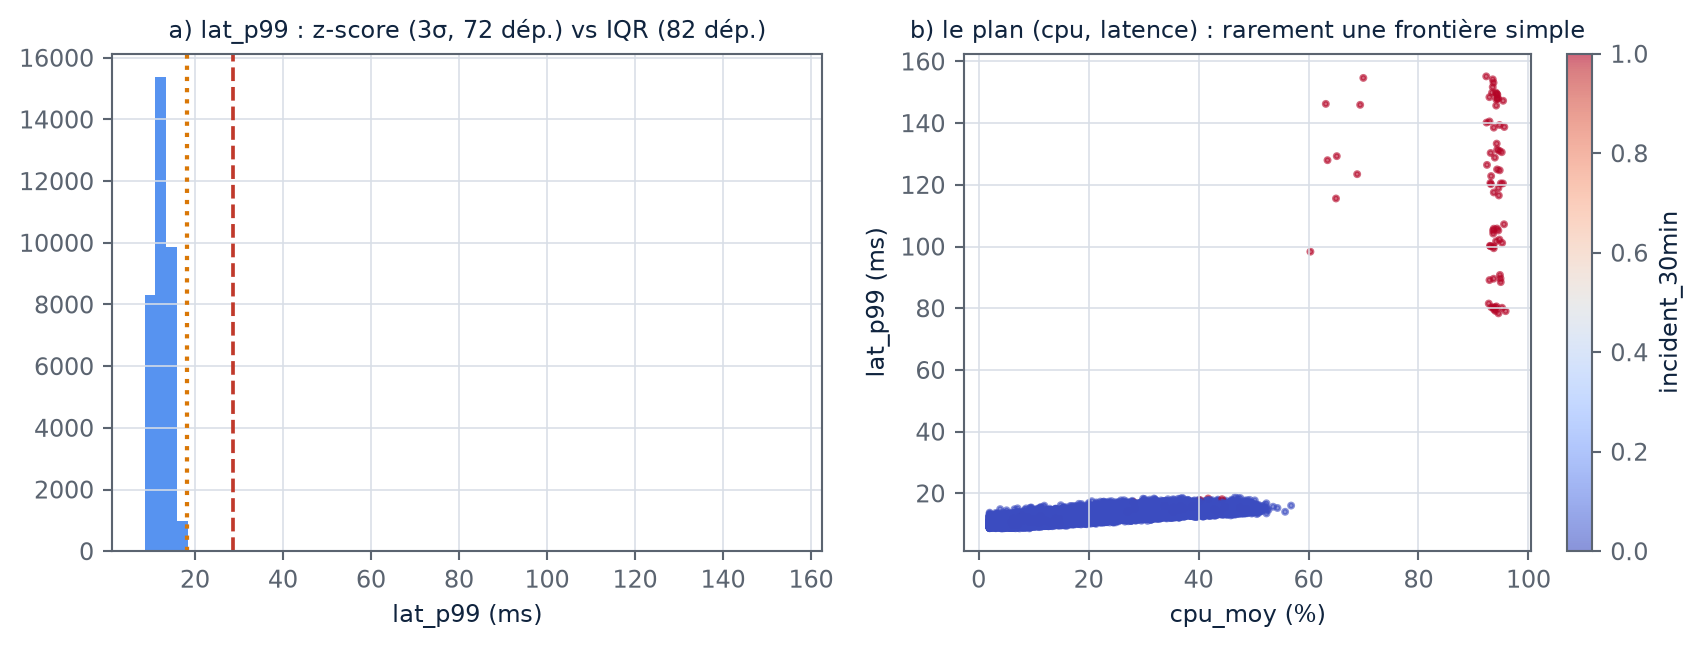
\includegraphics[width=\textwidth]{f16_seuils_statistiques.png}
\end{center}
\end{column}
\end{columns}
\end{frame}

\begin{frame}{IsolationForest : isoler plutôt que modéliser}
\footnotesize%
\begin{columns}[t]
\begin{column}{0.5\textwidth}
\begin{block}{Le principe en une phrase}
Une observation \textbf{rare} est isolée par \textbf{peu de coupes
aléatoires} ; une observation normale demande beaucoup de coupes.
\begin{itemize}
\item 300 arbres coupent l'espace au hasard ; la \textbf{profondeur
moyenne} d'isolement donne le \textbf{score d'anormalité}.
\item Aucune étiquette requise : apprentissage \textbf{non supervisé}.
\item \py{IsolationForest(contamination=0.01)} : contamination $=$
fraction d'anomalies \emph{attendue} --- elle fixe le seuil de décision.
\end{itemize}
\end{block}
\begin{kbox}[Pourquoi ça marche pour l'infra]
Le volume $(cpu, ram, latence, perte, temp)$ d'une fenêtre pré-incident
est \textbf{loin de tout le nuage} de fonctionnement normal : isolable
en peu de coupes, sans jamais avoir vu d'incident étiqueté.
\end{kbox}
\end{column}
\begin{column}{0.46\textwidth}
\begin{center}
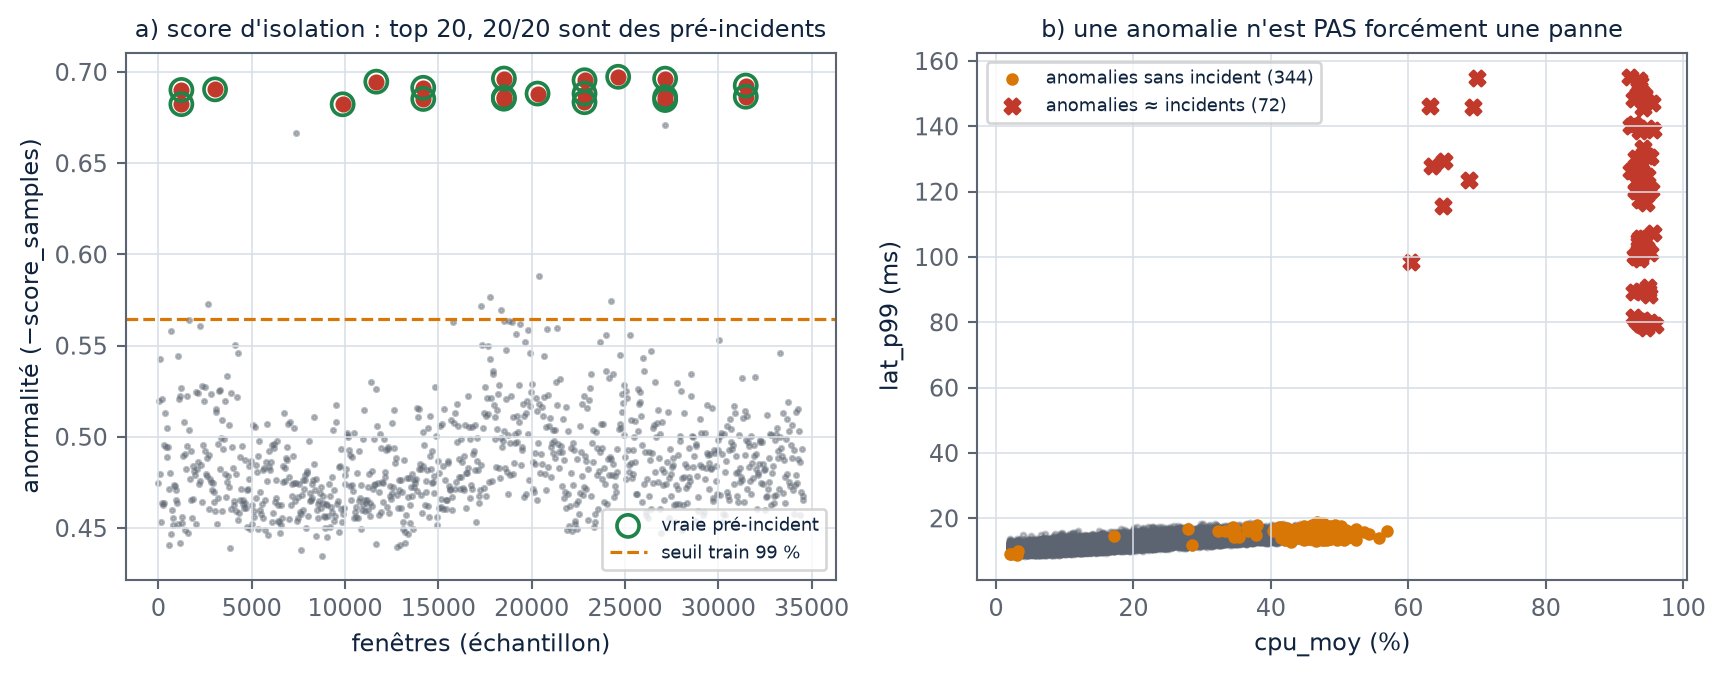
\includegraphics[width=\textwidth]{f17_isolation_forest.png}
\end{center}
\end{column}
\end{columns}
\end{frame}

\begin{frame}[fragile]{IsolationForest en 8 lignes}
\begin{codebox}[Le squelette à retenir]
\begin{lstlisting}
from sklearn.ensemble import IsolationForest

iso = IsolationForest(n_estimators=300,   # arbres
                      contamination=0.01, # seuil implicite
                      random_state=5534, n_jobs=2)
iso.fit(X_train_sans_etiquette)

score = -iso.score_samples(X)   # grand = anormal
anomalies = X[score > score[train].quantile(0.99)]
\end{lstlisting}
\end{codebox}
\begin{columns}[t]
\begin{column}{0.48\textwidth}
\begin{block}{Les 3 réglages qui comptent}
\begin{itemize}
\item \py{n\_estimators} : 300 suffit, au-delà score stable.
\item \py{contamination} : votre hypothèse de rareté --- à
justifier par le métier (ici $\approx$ 1 \%).
\item \py{random\_state=5534} : reproductibilité, comme partout.
\end{itemize}
\end{block}
\end{column}
\begin{column}{0.48\textwidth}
\begin{wbox}[Deux erreurs de débutant]
\begin{enumerate}
\item Entraîner sur \textbf{train+test} : le score du test est
alors contaminé par sa propre distribution.
\item Oublier \py{fillna} : \py{cpu\_delta} de la première fenêtre
est NaN --- sklearn refuse les NaN.
\end{enumerate}
\end{wbox}
\end{column}
\end{columns}
\end{frame}

\begin{frame}{Ce que l'IsolationForest trouve \emph{vraiment} (mesuré)}
\footnotesize%
\begin{columns}[t]
\begin{column}{0.52\textwidth}
\begin{ebox}[Résultats réels sur nosys\_features.csv]
Entraîné sur le train (24 192 fenêtres, \textbf{sans} la colonne
\py{incident\_30min}) :
\begin{itemize}
\item les \textbf{20 fenêtres les plus anormales} sont
\textbf{20/20} des pré-incidents (f17a) ;
\item mais au seuil « 1 \% du train », le test contient
\textbf{174 anomalies} dont seulement \textbf{40 incidents}
--- \textbf{134 fausses alarmes} (f17b).
\end{itemize}
\end{ebox}
\begin{wbox}[Piège n°1 : anomalie $\ne$ incident]
Une \textbf{anomalie} est un point statistiquement rare. Un
\textbf{incident} est une anomalie \emph{qui casse le service}.
Backup de nuit, pic de batch, déploiement : anormaux, bénins.
L'IsolationForest \textbf{name} le soupçon, il ne \textbf{classe} pas
la panne. C'est le travail du supervisé (cours 2).
\end{wbox}
\end{column}
\begin{column}{0.44\textwidth}
\begin{block}{LOF : la densité locale (complément)}
Le LOF (Local Outlier Factor) compare la densité \textbf{autour} d'un
point à celle de ses voisins : utile quand les clusters normaux ont des
\textbf{densités très différentes} (nuit vs pic de journée).
\begin{itemize}
\item LOF $\approx 1$ : densité normale ; LOF $\gg 1$ : hors densité.
\item Sur nosys, IsolationForest et LOF pointent essentiellement les
mêmes fenêtres --- on retient IsolationForest, scalable et parallèle
(\py{n\_jobs=2}).
\end{itemize}
\end{block}
\end{column}
\end{columns}
\end{frame}

\begin{frame}{Scores, seuils : qui décide de « alerte » ?}
\begin{columns}[t]
\begin{column}{0.48\textwidth}
\begin{block}{La chaîne complète}
score brut $s(x)$ $\Rightarrow$ seuil $t$ $\Rightarrow$ décision
$s(x) \ge t$.
\begin{itemize}
\item \textbf{z-score / IQR} : seuil implicite (3$\sigma$, 1,5 IQR).
\item \textbf{IsolationForest} : seuil $=$ quantile du score sur le
train (1 \% ici) ou paramètre \py{contamination}.
\item \textbf{Supervisé} : seuil sur la probabilité prédite ---
cours 2 et TP B4.
\end{itemize}
\end{block}
\end{column}
\begin{column}{0.48\textwidth}
\begin{kbox}[Le seuil est un choix MÉTIER, pas statistique]
Descendre le seuil $=$ plus de rappel, plus de fatigue NOC.
Le monter $=$ moins de bruit, incidents manqués.
Il n'existe \textbf{pas} de seuil optimal universel : il y a un seuil
par \textbf{budget d'opérateurs}. Le TP B4 le chiffre : 5 alertes
/jour/serveur maximum.
\end{kbox}
\end{column}
\end{columns}
\end{frame}

\begin{frame}{Quiz 1 --- anomalies non supervisées (5 min)}
\begin{qbox}[3 questions]
\begin{enumerate}
\item Une fenêtre anormale selon IsolationForest est :\\
(a) forcément un incident \quad (b) statistiquement rare --- à vérifier
contre les alarmes réelles \quad (c) une panne confirmée
\item Le paramètre \py{contamination} sert à :\\
(a) initialiser les arbres \quad (b) fixer la fraction d'anomalies
attendue, donc le seuil \quad (c) paralléliser
\item Pourquoi le z-score suffit-il rarement seul ?\\
(a) trop lent \quad (b) une variable à la fois, seuil arbitraire,
ignore les combinaisons \quad (c) il exige des étiquettes
\end{enumerate}
\end{qbox}
\vspace{1mm}
\begin{solbox}[Réponses]
\textbf{1 : b} \quad \textbf{2 : b} \quad \textbf{3 : b} --- d'où le
passage au modèle joint et supervisé.
\end{solbox}
\end{frame}

% =====================================================================
%  Seance 3 -- B. cours 2 : classification sur classe rare (frames 10--18)
% =====================================================================
\section{Classification supervisée sur classe rare}

\begin{frame}{Le problème : 0,35 \% de positifs}
\footnotesize%
\begin{columns}[t]
\begin{column}{0.5\textwidth}
\begin{center}
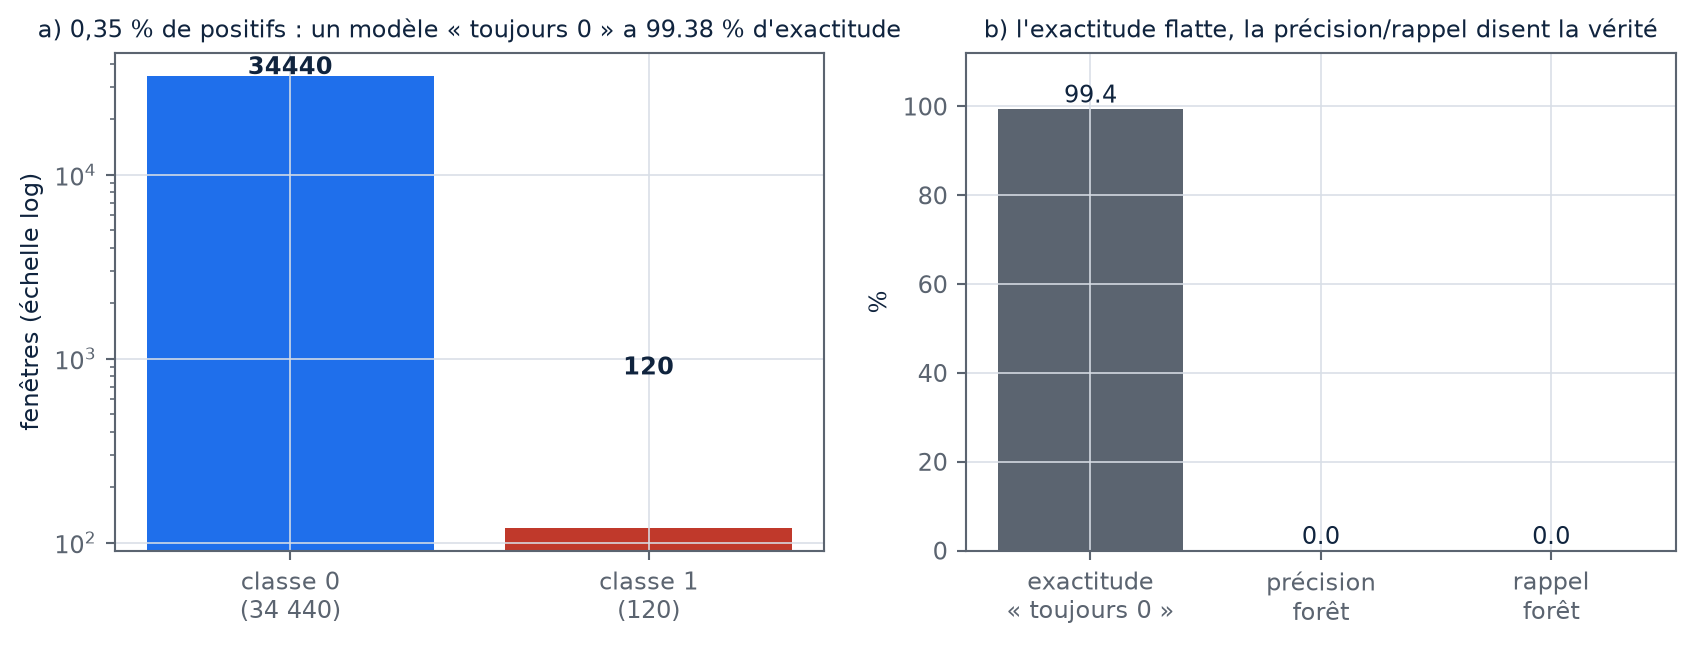
\includegraphics[width=\textwidth]{f18_desequilibre.png}
\end{center}
\end{column}
\begin{column}{0.46\textwidth}
\begin{block}{Le split temporel, seul valable}
\begin{center}\small
\begin{tabular}{@{}lll@{}}
\toprule
 & fenêtres & positifs\\
\midrule
train $<$ 22/09 & 24 192 & 56\\
test $\ge$ 22/09 & 10 368 & 64\\
\bottomrule
\end{tabular}
\end{center}
Le test contient l'incident du 22/09 à 3 h : le modèle est jugé sur
un \textbf{futur jamais vu}.
\end{block}
\begin{wbox}[L'exactitude est trompeuse]
Un modèle « toujours 0 » atteint \textbf{99,65 \%} d'exactitude
(34 440 / 34 560) --- et ne détecte \textbf{rien}. À cette rareté,
l'exactitude ne mesure plus rien : il faut la matrice de confusion.
\end{wbox}
\end{column}
\end{columns}
\end{frame}

\begin{frame}[fragile]{Les 4 modèles, entraînés pour de vrai}
\begin{codebox}[Le même protocole pour les quatre --- split temporel strict]
\begin{lstlisting}
from sklearn.linear_model import LogisticRegression
from sklearn.ensemble import (RandomForestClassifier,
                              GradientBoostingClassifier)
from sklearn.preprocessing import StandardScaler

Xtr, ytr = X[train], f.loc[train, "incident_30min"]
Xte, yte = X[~train], f.loc[~train, "incident_30min"]

rf = RandomForestClassifier(300, class_weight="balanced",
                            random_state=5534, n_jobs=2)
gb = GradientBoostingClassifier(random_state=5534)
sc = StandardScaler().fit(Xtr)          # statistiques du TRAIN
lr = LogisticRegression(class_weight="balanced",
                        max_iter=3000).fit(sc.transform(Xtr), ytr)
\end{lstlisting}
\end{codebox}
\begin{wbox}[Où la fuite se cache quand on standardise]
\py{StandardScaler().fit(X)} sur train+test mélangés importe la
moyenne \emph{du futur} dans le passé. Toujours \textbf{fit sur
le train}, \py{transform} sur les deux. Même règle pour tout
statistique appris (seuil, quantile, moyenne mobile).
\end{wbox}
\end{frame}

\begin{frame}{La matrice de confusion : le seul regard honnête}
\footnotesize%
\begin{columns}[t]
\begin{column}{0.42\textwidth}
\begin{center}\small
\begin{tabular}{@{}lp{2.0cm}p{2.0cm}@{}}
\toprule
 & prédit 0 & prédit 1\\
\midrule
réel 0 & \textbf{TN} juste & \textbf{FP} fausse alarme\\
réel 1 & \textbf{FN} manqué & \textbf{TP} détecté\\
\bottomrule
\end{tabular}
\end{center}
\vspace{1mm}
\begin{block}{Les deux métriques qui comptent}
\begin{itemize}
\item \textbf{Précision} $= TP/(TP{+}FP)$ : quand ça alerte, à quel
point c'est vrai ? $\rightarrow$ fatigue du NOC.
\item \textbf{Rappel} $= TP/(TP{+}FN)$ : quelle part des incidents
est vue ? $\rightarrow$ SLA.
\item $F_1 = 2\,\dfrac{p \times r}{p + r}$ : compromis unique.
\end{itemize}
\end{block}
\end{column}
\begin{column}{0.54\textwidth}
\begin{center}
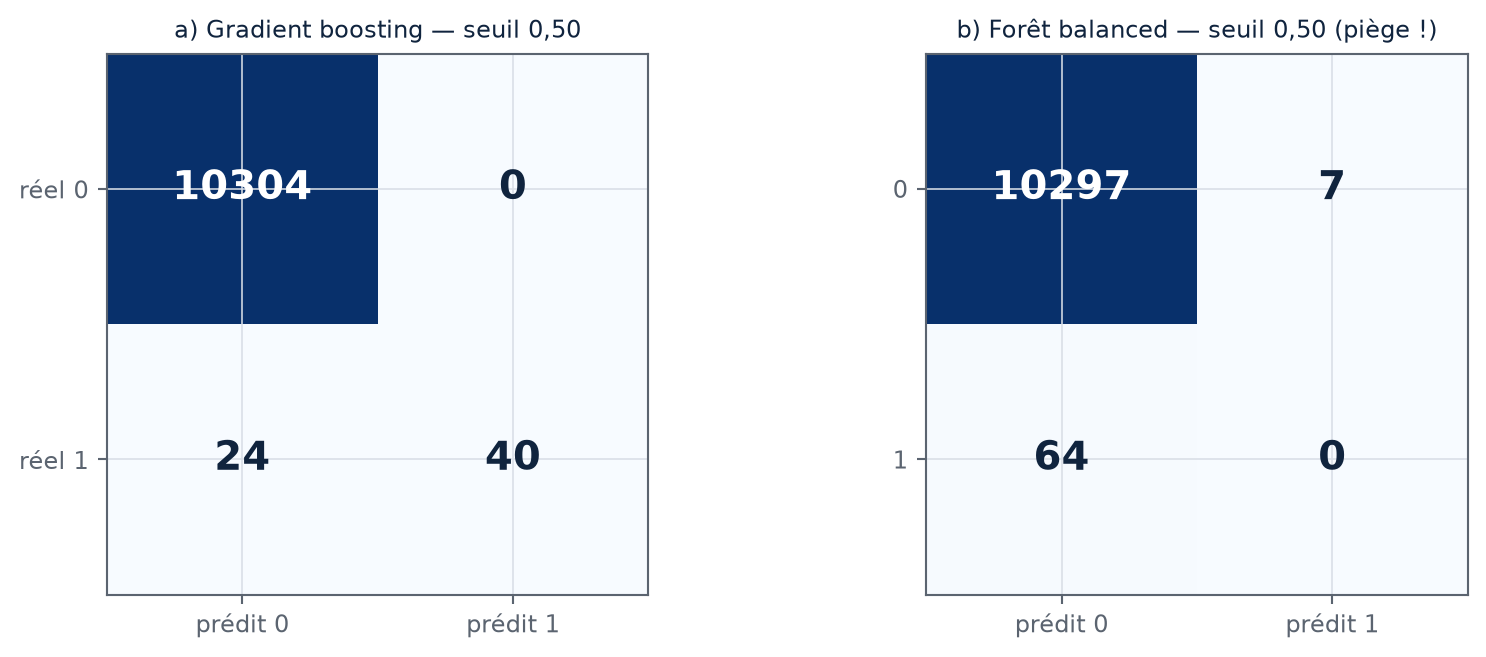
\includegraphics[width=\textwidth]{f19_matrice_confusion.png}
\end{center}
\begin{kbox}[Mesuré sur le test]
Gradient boosting, seuil 0,50 : \textbf{40 TP, 0 FP, 24 FN} ---
précision 1,00, rappel 0,625, $F_1$ 0,769 (chiffres réels du JSON).
\end{kbox}
\end{column}
\end{columns}
\end{frame}

\begin{frame}{Les 4 familles de modèles, en une slide chacune}
\footnotesize%
\begin{columns}[t]
\begin{column}{0.48\textwidth}
\begin{block}{Régression logistique}
\begin{itemize}
\item $p(\text{incident}) = \sigma(w \cdot x)$ : linéaire, calibrée,
\textbf{interprétable} (chaque poids = effet d'une variable).
\item Rapide, stable, mais rate les frontières non linéaires.
\end{itemize}
\end{block}
\begin{block}{Arbre de décision}
\begin{itemize}
\item Règles \emph{ lisibles} : « si \py{lat\_p99} $>$ 20 et
\py{perte\_moy} $>$ 0,5 alors alerte ».
\item Seul, il sur-apprend : profond = bruit mémorisé.
\end{itemize}
\end{block}
\end{column}
\begin{column}{0.48\textwidth}
\begin{block}{Forêt aléatoire}
\begin{itemize}
\item Moyenne de 300 arbres sur échantillons/variables aléatoires :
\textbf{robuste}, peu de réglage, donne des \textbf{importances}.
\item \py{class\_weight='balanced'} : les 56 exemples du train
pèsent comme $\approx$ 12 000 négatifs.
\end{itemize}
\end{block}
\begin{block}{Gradient boosting}
\begin{itemize}
\item Arbres \emph{successifs} qui corrigent chacun les erreurs des
précédents : souvent le \textbf{meilleur} sur tabulaire.
\item Plus sensible au réglage, moins parallélisable.
\end{itemize}
\end{block}
\end{column}
\end{columns}
\end{frame}

\begin{frame}{Classe rare : \py{class\_weight='balanced'} vs SMOTE}
\footnotesize%
\begin{columns}[t]
\begin{column}{0.5\textwidth}
\begin{block}{class\_weight='balanced' (retenu)}
\begin{itemize}
\item Pèse la fonction de coût : une erreur sur la classe rare
compte $\approx \dfrac{N}{2 \times N_{min}}$ fois plus.
\item Aucune donnée synthétique : \textbf{pas de risque de fuite}
ni d'artefacts.
\item Effet mesuré ici : le seuil de décision effectif se déplace
--- à 0,50 la forêt balanced est \emph{trop} agressive
(précision 0,00 sur le test).
\end{itemize}
\end{block}
\end{column}
\begin{column}{0.46\textwidth}
\begin{block}{SMOTE (mention)}
\begin{itemize}
\item Crée des exemples minoritaires \textbf{synthétiques} par
interpolation entre voisins rares.
\item DANGER en séries temporelles : interpoler entre deux
fenêtres de \emph{serveurs différents} ou de \emph{jours différents}
fabrique des points qui ne peuvent pas exister.
\item Retenu : \py{class\_weight}, plus simple et sûr ici.
\end{itemize}
\end{block}
\end{column}
\end{columns}
\end{frame}

\begin{frame}{Quiz 2 --- classe rare (5 min)}
\begin{qbox}[3 questions]
\begin{enumerate}
\item Un modèle « toujours 0 » sur notre dataset a une exactitude de :\\
(a) 50 \% \quad (b) 99,65 \% \quad (c) 0,35 \%
\item Précision 1,0 et rappel 0,1 signifie :\\
(a) le modèle est parfait \quad (b) chaque alerte est vraie, mais
9 incidents sur 10 sont manqués \quad (c) il n'alerte jamais
\item En série temporelle, SMOTE est risqué car :\\
(a) il est lent \quad (b) il fabrique des fenêtres synthétiques
sans réalité physique ni cohérence temporelle \quad (c) il exige
des étiquettes
\end{enumerate}
\end{qbox}
\vspace{1mm}
\begin{solbox}[Réponses]
\textbf{1 : b} (34 440 / 34 560) \quad \textbf{2 : b} \quad \textbf{3 : b}
\end{solbox}
\end{frame}

\begin{frame}{Précision-rappel bat la courbe ROC ici}
\footnotesize%
\begin{columns}[t]
\begin{column}{0.48\textwidth}
\begin{center}
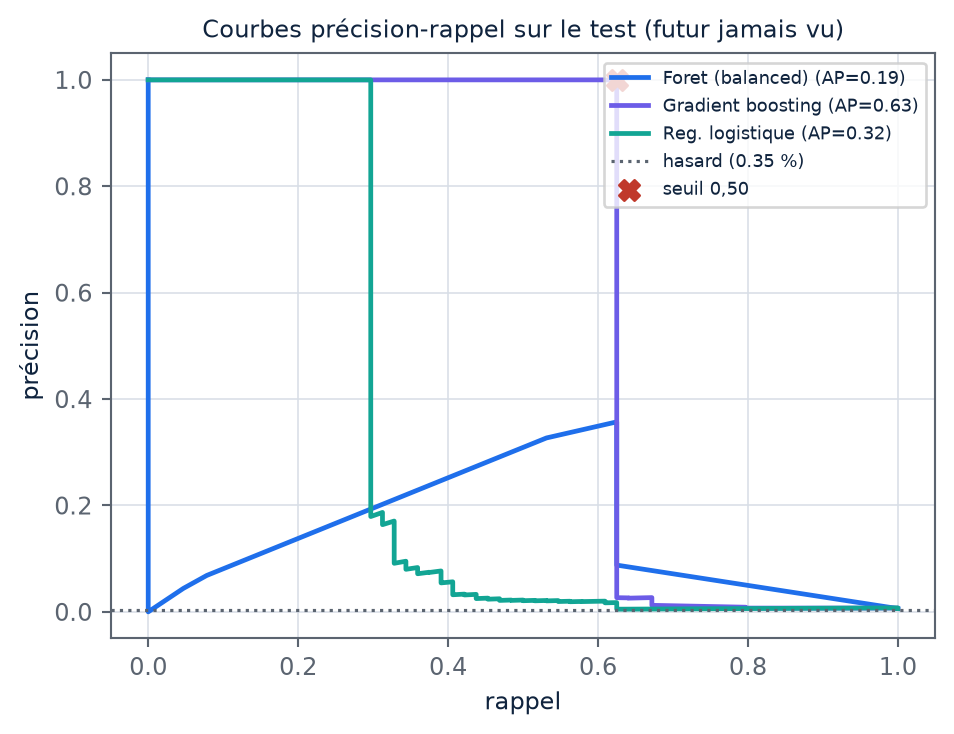
\includegraphics[width=\textwidth]{f20_courbes_pr.png}
\end{center}
\end{column}
\begin{column}{0.48\textwidth}
\begin{block}{Pourquoi pas la ROC / AUC ?}
La ROC utilise \textbf{FPR} $= FP/(FP{+}TN)$ : avec 10 304 négatifs,
même 300 fausses alarmes donnent un FPR minuscule $\Rightarrow$
la ROC \textbf{flatte} les modèles sur classes très rares.
\end{block}
\begin{kbox}[La courbe PR, elle, parle métier]
Chaque point $=$ un couple (fatigue NOC, SLA). La ligne pointillée
est le \textbf{hasard} (0,35 \%). Mesuré : gradient boosting
\textbf{AP = 0,63}, forêt 0,19, logistique 0,32 --- l'écart se lit
directement en « alertes utiles par jour ».
\end{kbox}
\begin{wbox}[Coût asymétrique]
\textbf{FP} : opérationnel dérangé pour rien --- fatigue,
désensibilisation. \textbf{FN} : SLA cassé (99,80 \% mesuré).
Ici le FN coûte plus cher, mais un flux de FP détruit la
confiance en l'outil.
\end{wbox}
\end{column}
\end{columns}
\end{frame}

% =====================================================================
%  Seance 3 -- C. cours 3 : choisir le modele (frames 19--23)
% =====================================================================
\section{Choisir le modèle : validation temporelle et interprétabilité}

\begin{frame}{Le protocole d'évaluation, récapitulé}
\begin{columns}[t]
\begin{column}{0.5\textwidth}
\begin{block}{Les 5 règles non négociables}
\begin{enumerate}
\item \textbf{Split temporel} : train $<$ 22/09, test $\ge$ 22/09.
Le test contient l'incident du 22/09 3 h.
\item \textbf{Tout statistique appris} (scaler, seuil, quantile)
se calcule sur le train seul.
\item \textbf{Validation croisée temporelle} sur le train ;
jamais de KFold mélangé.
\item \textbf{Métriques de classe rare} : précision, rappel,
$F_1$, courbe PR --- pas l'exactitude, pas la ROC.
\item \textbf{Seuil choisi sur contrainte métier} (budget NOC),
pas sur un réflexe 0,50.
\end{enumerate}
\end{block}
\end{column}
\begin{column}{0.46\textwidth}
\begin{kbox}[Ce protocole vaut pour toute l'industrie]
Les mêmes 5 règles s'appliquent à la détection de fraude,
de churn, de défaut de paiement : classe rare + données
ordonnées dans le temps $=$ le cas d'usage le plus fréquent
du ML applicatif. Ce que vous validez ce soir se retrouve
dans chaque projet de production.
\end{kbox}
\begin{wbox}[Le test du test]
Avant de croire vos chiffres, demandez : « mon modèle aurait-il
pu voir ces données à l'entraînement ? » Si la réponse n'est pas
un \textbf{non} franc, votre évaluation est optimiste.
\end{wbox}
\end{column}
\end{columns}
\end{frame}

\begin{frame}[fragile]{Validation croisée TEMPORELLE : jamais de KFold mélangé}
\footnotesize%
\begin{codebox}[TimeSeriesSplit : le futur reste hors d'atteinte]
\begin{lstlisting}
from sklearn.model_selection import TimeSeriesSplit
tsc = TimeSeriesSplit(n_splits=5)      # plis CHRONOLOGIQUES
for tr_i, va_i in tsc.split(Xtr):      # va_i est APRES tr_i
    modele.fit(Xtr[tr_i], ytr[tr_i])
    pred = modele.predict_proba(Xtr[va_i])[:, 1]
\end{lstlisting}
\end{codebox}
\begin{columns}[t]
\begin{column}{0.48\textwidth}
\begin{wbox}[Pourquoi KFold mélangé est une triche]
Séance 2 : les fenêtres sont \textbf{autocorrélées} (moyennes
mobiles, tendance). Un pli mélangé contient le \textbf{voisin
direct} d'une fenêtre du train : le modèle « devine » par
continuité et paraît excellent --- jusqu'à la production.
\end{wbox}
\end{column}
\begin{column}{0.48\textwidth}
\begin{ebox}[Mesuré (5 plis temporels, F1 moyen ± écart-type)]
\begin{center}\small
\begin{tabular}{@{}l l@{}}
\toprule
Gradient boosting & \textbf{0,715 ± 0,024}\\
Forêt (balanced) & 0,343 ± 0,299\\
Reg. logistique & 0,247 ± 0,213\\
\bottomrule
\end{tabular}
\end{center}
Le fort écart-type de la forêt signale un modèle
\textbf{instable selon la période} --- information que la moyenne
seule cacherait.
\end{ebox}
\end{column}
\end{columns}
\end{frame}

\begin{frame}{Le match final, chiffres réels sur le test}
\begin{center}
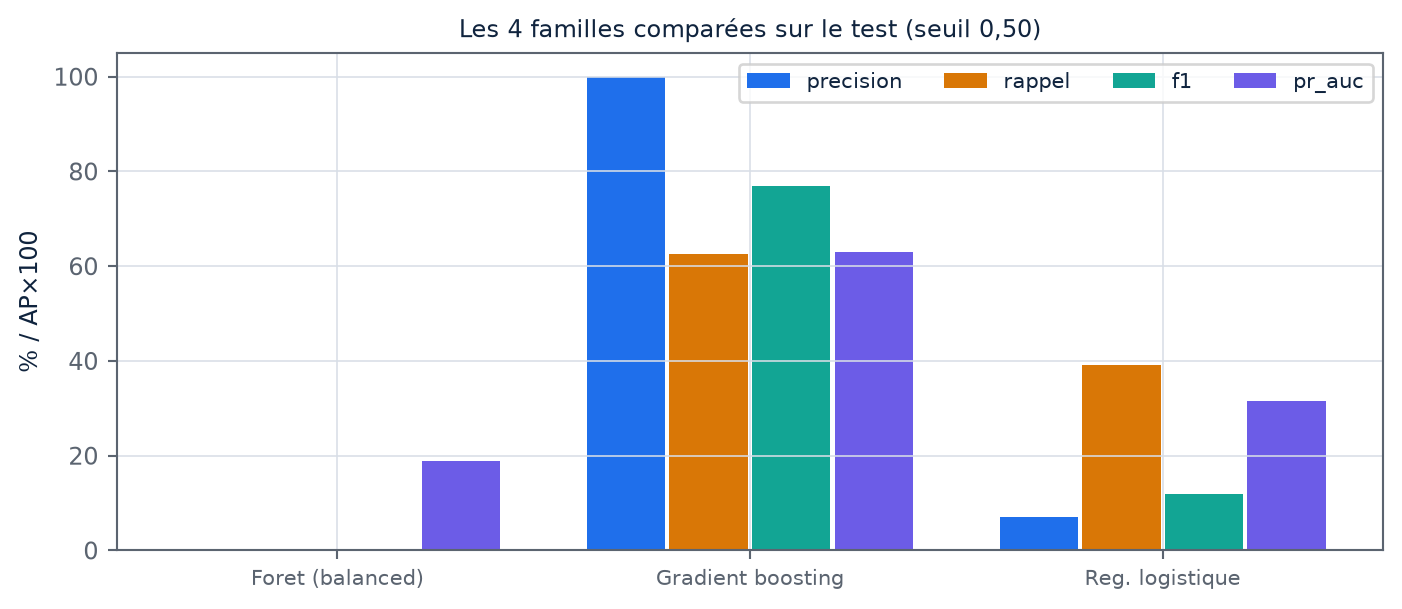
\includegraphics[width=0.60\textwidth]{f21_comparaison_modeles.png}
\end{center}
\vspace{0.5mm}
\begin{center}\footnotesize
\begin{tabular}{@{}l c c c c@{}}
\toprule
Modèle (test, seuil 0,50) & Précision & Rappel & $F_1$ & AP (courbe PR)\\
\midrule
Gradient boosting & \textbf{1,00} & \textbf{0,625} & \textbf{0,769} & \textbf{0,63}\\
Reg. logistique & 0,07 & 0,39 & 0,12 & 0,32\\
Forêt (balanced) & 0,00 & 0,00 & 0,00 & 0,19\\
\bottomrule
\end{tabular}
\end{center}
\vspace{0.5mm}
\begin{wbox}[Leçon du piège balanced]
À 0,50, la forêt balanced prédit 7 positifs... tous faux : avec des
poids rééquilibrés, \textbf{le seuil par défaut perd son sens} ---
re-choisir le seuil sur la courbe PR (TP B4).
\end{wbox}
\end{frame}

\begin{frame}{Interprétabilité : les arbres parlent au métier}
\footnotesize%
\begin{columns}[t]
\begin{column}{0.5\textwidth}
\begin{center}
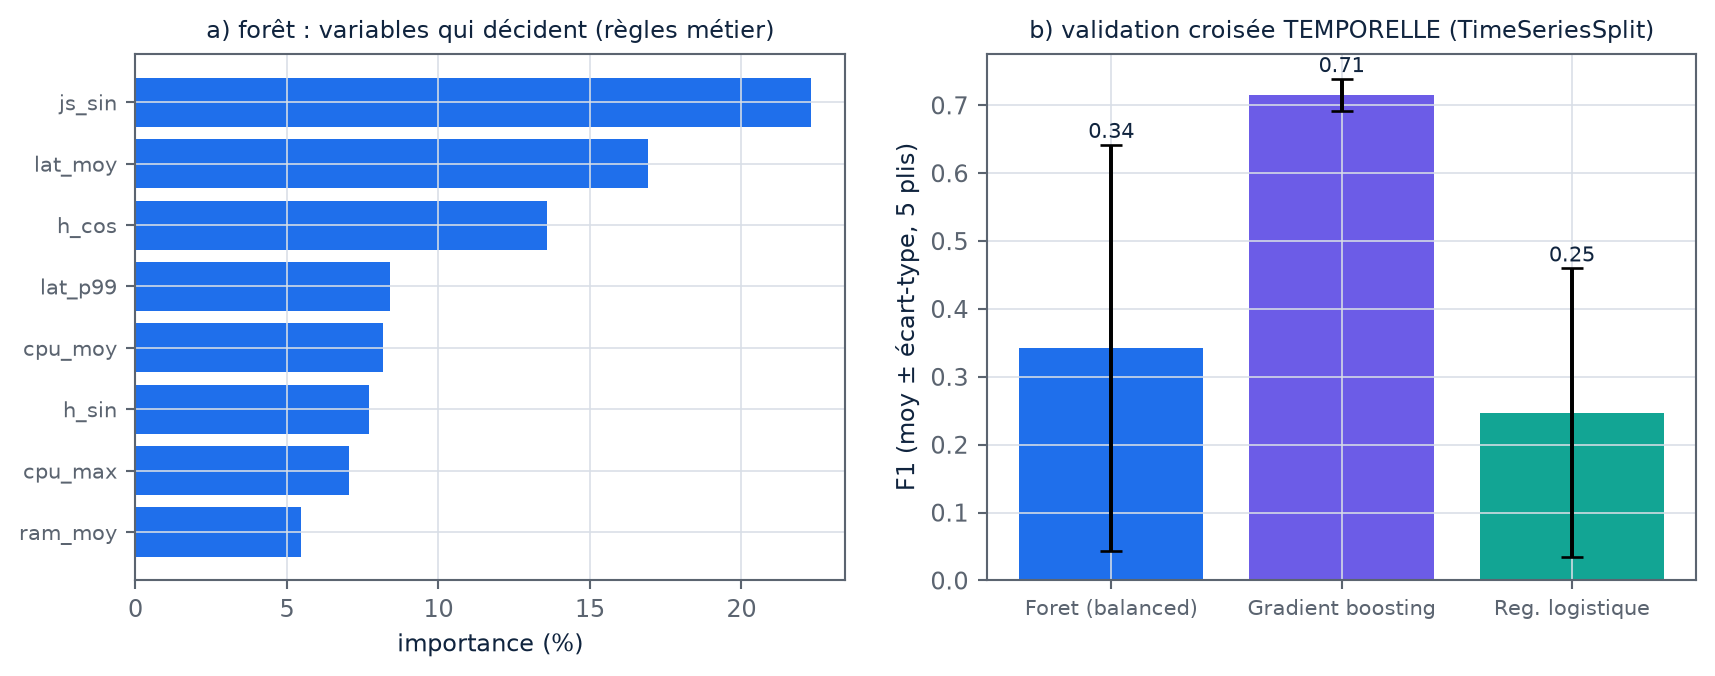
\includegraphics[width=\textwidth]{f23_interpretabilite_cv.png}
\end{center}
\end{column}
\begin{column}{0.46\textwidth}
\begin{block}{Ce que la forêt expose}
Les importances désignent les variables qui décident (f23a) ---
de quoi écrire des \textbf{règles métier} auditables par
l'exploitant : « si latence p99 haut \textbf{et} perte non nulle
\textbf{alors} fenêtre à risque ».
\end{block}
\begin{kbox}[Compromis à assumer]
\begin{itemize}
\item \textbf{Logistique} : la plus lisible, la moins juste.
\item \textbf{Arbre} : règles lisibles, fragile seul.
\item \textbf{Forêt/boosting} : les plus justes, boîte grise ---
explication partielle via les importances.
\end{itemize}
\end{kbox}
\end{column}
\end{columns}
\end{frame}

\begin{frame}{Quiz 3 --- choisir et valider (5 min)}
\begin{qbox}[3 questions]
\begin{enumerate}
\item Pour valider un modèle sur nos 30 jours de métriques, on utilise :\\
(a) KFold mélangé, plus précis \quad (b) \py{TimeSeriesSplit}, plis
chronologiques \quad (c) un seul split au hasard
\item Le gradient boosting gagne en AP (0,63 vs 0,19). Que lit-on
dans une courbe PR que la ROC cache ?\\
(a) la vitesse \quad (b) le couple concret précision/rappel à chaque
seuil --- l'ASP ne s'effondre pas avec les 10 000 négatifs \quad
(c) la mémoire utilisée
\item Pourquoi garder la régression logistique malgré son $F_1$ de 0,12 ?\\
(a) elle est jolie \quad (b) baseline interprétable : chaque poids
explique l'effet d'une variable, référence pour juger les autres \quad
(c) elle n'a pas besoin de seuil
\end{enumerate}
\end{qbox}
\vspace{1mm}
\begin{solbox}[Réponses]
\textbf{1 : b} --- l'autocorrélation temporelle tricherait sinon.
\quad \textbf{2 : b} \quad \textbf{3 : b} --- toujours une baseline
lisible en concurrence.
\end{solbox}
\end{frame}

% =====================================================================
%  Seance 3 -- D. TP : detecter les incidents avant la panne (frames 24--30)
% =====================================================================
\section{TP « Détecter les incidents avant la panne »}

\begin{frame}{Le TP : objectif et règle du jeu}
\footnotesize%
\begin{columns}[t]
\begin{column}{0.5\textwidth}
\begin{kbox}[Ce que vous produisez à 18 h]
Un \textbf{système d'alerte} sur \file{nosys\_features.csv} qui :
\begin{enumerate}
\item détecte sans étiquette (IsolationForest) ;
\item prédit « incident $\le$ 30 min » avec un modèle supervisé ;
\item respecte un \textbf{budget NOC} : $\le$ 5 alertes/jour/serveur ;
\item est \textbf{justifié par les chiffres} : matrice de confusion,
courbe PR, tableau comparatif.
\end{enumerate}
\end{kbox}
\begin{ebox}[Rappels de cadrage]
\begin{itemize}
\item Split \textbf{temporel} imposé : train $<$ 22/09 (24 192),
test $\ge$ 22/09 (10 368, 9 jours).
\item Graine 5534 partout (\py{random\_state=5534}).
\item Jamais de KFold mélangé.
\end{itemize}
\end{ebox}
\end{column}
\begin{column}{0.46\textwidth}
\begin{center}
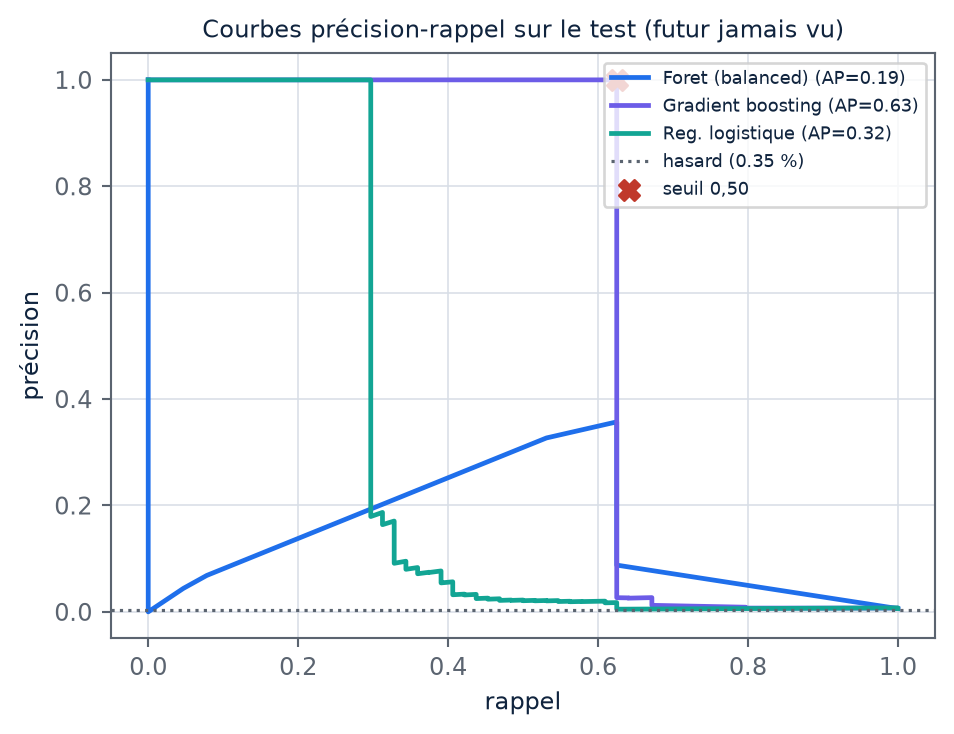
\includegraphics[width=\textwidth]{f20_courbes_pr.png}
\end{center}
\vspace{1mm}
\begin{center}\small
Votre cible à battre (corrigé officiel) :\\ $F_1$ \textbf{0,769},
rappel \textbf{0,625}, AP \textbf{0,63}.
\end{center}
\end{column}
\end{columns}
\end{frame}

\begin{frame}[fragile]{TP B1 --- IsolationForest sans étiquette (25 min)}
\begin{codebox}[B1. Détecter sans jamais regarder la cible]
\begin{lstlisting}
import pandas as pd
from sklearn.ensemble import IsolationForest

f = pd.read_csv("data/nosys_features.csv", parse_dates=["fenetre"])
X = f.drop(columns=["serveur", "fenetre", "incident_30min"])
X = X.fillna(0.0)                       # cpu_delta de la 1re fenetre

train = f["fenetre"] < "2026-09-22"
iso = IsolationForest(n_estimators=300, contamination=0.01,
                      random_state=5534, n_jobs=2).fit(X[train])
f["score_anomalie"] = -iso.score_samples(X)

top20 = f.nlargest(20, "score_anomalie")
print(top20[["serveur", "fenetre", "cpu_moy", "lat_p99",
             "incident_30min"]])
\end{lstlisting}
\end{codebox}
\begin{abox}[Livrable B1]
La liste des 20 fenêtres les plus anormales, triée par score.
Contrôle attendu (corrigé) : \textbf{20/20 sont des pré-incidents}.
Notez à la main ce que vous \emph{pouviez} savoir : aucun
\py{incident\_30min} n'est entré dans le calcul.
\end{abox}
\end{frame}

\begin{frame}[fragile]{TP B2 --- recouvrement détections / alarmes réelles (20 min)}
\begin{codebox}[B2. Confronter le non-supervisé au réel]
\begin{lstlisting}
seuil = f.loc[train, "score_anomalie"].quantile(0.99)
f["anomalie"] = f["score_anomalie"] > seuil

test = f[~train]
print("anomalies test :", test["anomalie"].sum())      # 174
print("dont vrais incidents :",
      test.loc[test["anomalie"], "incident_30min"].sum())  # 40

# recouvrement : par fenetre, combien de serveurs detectes ?
cov = (test.groupby("fenetre")["anomalie"].sum()
           .value_counts().sort_index())
print(cov)     # incidents vus sur 1, 2, ... serveurs a la fois
\end{lstlisting}
\end{codebox}
\begin{columns}[t]
\begin{column}{0.48\textwidth}
\begin{wbox}[Ce que 174 anomalies veulent dire]
\textbf{40} correspondent à un incident à venir ; les
\textbf{134} autres sont des anomalies bénignes (batch, backup,
pics). Chaque fausse alerte coûte une nuit d'ingénieur : le
non-supervisé seul ne suffit pas.
\end{wbox}
\end{column}
\begin{column}{0.48\textwidth}
\begin{ebox}[Livrable B2]
Un tableau croisé (anomalie $\times$ incident) sur le test + un
commentaire de 3 lignes : quelle part des anomalies vaut le coup
d'être envoyée au NOC ?
\end{ebox}
\end{column}
\end{columns}
\end{frame}

\begin{frame}[fragile]{TP B3 --- forêt balanced et matrice de confusion (30 min)}
\begin{codebox}[B3. Entraîner, puis JUGER sur le futur]
\begin{lstlisting}
from sklearn.ensemble import RandomForestClassifier
from sklearn.metrics import confusion_matrix

Xtr, ytr = X[train], f.loc[train, "incident_30min"]
Xte, yte = X[~train], f.loc[~train, "incident_30min"]

rf = RandomForestClassifier(n_estimators=300,
        class_weight="balanced", random_state=5534,
        n_jobs=2).fit(Xtr, ytr)
proba = rf.predict_proba(Xte)[:, 1]
pred  = (proba >= 0.5).astype(int)

print(confusion_matrix(yte, pred))
\end{lstlisting}
\end{codebox}
\begin{columns}[t]
\begin{column}{0.48\textwidth}
\begin{wbox}[Le piège que vous devez rencontrer]
Avec \py{class\_weight='balanced'}, le seuil 0,50 n'est plus
calibré : au corrigé, la forêt prédit 7 positifs... tous faux
(précision 0,00). Ce n'est \textbf{pas un bug} : c'est le déplacement
du seuil effectif. Ne paniquez pas, passez au B4.
\end{wbox}
\end{column}
\begin{column}{0.48\textwidth}
\begin{ebox}[Livrable B3]
La matrice de confusion sur le test + les 4 cadres
(TN/FP/FN/TP) commentés en coût métier : qui dérange qui,
combien de SLA en jeu.
\end{ebox}
\end{column}
\end{columns}
\end{frame}

\begin{frame}[fragile]{TP B4 --- courbe PR et seuil métier (30 min)}
\begin{codebox}[B4. Choisir le seuil sous contrainte de budget NOC]
\begin{lstlisting}
from sklearn.metrics import precision_recall_curve
prec, rec, thr = precision_recall_curve(yte, proba)

# budget : 5 alertes/jour/serveur
# test = 9 jours x 8 serveurs -> au plus 5*8*9 = 360 alertes
def alertes_jour_serveur(s):
    n = (proba >= s).sum()          # alertes sur tout le test
    return n / 9 / 8                # par jour et par serveur

for s in [0.5, 0.2, 0.1, 0.05, 0.02, 0.01]:
    p = (proba >= s).astype(int)
    print(s, alertes_jour_serveur(s),
          precision_score(yte, p, zero_division=0),
          recall_score(yte, p, zero_division=0))
\end{lstlisting}
\end{codebox}
\begin{abox}[Livrable B4]
La courbe précision-rappel de VOTRE modèle + le tableau
seuil $\rightarrow$ (alertes/jour/serveur, précision, rappel), et le
\textbf{seuil recommandé} qui respecte les 5 alertes/jour/serveur.
Référence du corrigé (gradient boosting) : \textbf{40 alertes sur
9 jours} $= 0{,}56$/jour/serveur, précision 1,00, rappel 0,625.
\end{abox}
\end{frame}

\begin{frame}{TP B5 --- livrable et barème}
\begin{columns}[t]
\begin{column}{0.52\textwidth}
\begin{abox}[À rendre]
\begin{enumerate}
\item \textbf{Tableau comparatif} des modèles (au moins
logistique, forêt, boosting --- et IsolationForest en repère) :
précision, rappel, $F_1$, AP, alertes/jour/serveur au seuil choisi.
\item \textbf{Seuil recommandé} avec sa justification métier
(budget NOC, coût FP vs FN).
\item \textbf{Un paragraphe} (5--8 lignes) : quel modèle vous
déployez, pourquoi, et ce que vous n'avez PAS détecté (les 24 FN
du corrigé --- que farez-vous ?).
\item Reproductibilité : graine 5534, split temporel cité.
\end{enumerate}
\end{abox}
\end{column}
\begin{column}{0.44\textwidth}
\begin{kbox}[Barème (20 pts)]
\begin{itemize}
\item B1 IsolationForest sans fuite --- 3 pts
\item B2 recouvrement + commentaire honnête --- 3 pts
\item B3 forêt balanced + matrice juste --- \textbf{5 pts}
\item B4 courbe PR + seuil sous budget --- \textbf{5 pts}
\item B5 comparatif + argumentation métier --- 3 pts
\item Reproductibilité (graine, split) --- 1 pt
\end{itemize}
\end{kbox}
\begin{wbox}[Fuite = 0 au critère B3]
Toute valeur calculée sur train+test mélangés (standardisation,
seuil, SMOTE) annule le critère : le futur ne sert qu'à juger.
\end{wbox}
\end{column}
\end{columns}
\end{frame}

% =====================================================================
%  Seance 3 -- E. synthese, reponse a la seance 1, preview (frames 31--35)
% =====================================================================
\section{Synthèse de la séance 3}

\begin{frame}{Quiz de synthèse --- 6 questions (10 min)}
\begin{qbox}[Répondez seul(e), puis correction]
\begin{enumerate}
\item L'IsolationForest est entraîné :\\
(a) sur les features SANS l'étiquette \quad (b) sur train+test
avec étiquette \quad (c) uniquement sur les incidents
\item 174 anomalies test mais 40 incidents : les 134 autres sont :\\
(a) des bugs \quad (b) des anomalies bénignes (batch, backup) \quad
(c) des fuites
\item La précision d'un détecteur mesure :\\
(a) la part des incidents vus \quad (b) la part des alertes
qui sont de vrais incidents \quad (c) la vitesse
\item Quelle courbe préférer à 0,35 \% de positifs ?\\
(a) ROC/AUC \quad (b) précision-rappel \quad (c) courbe de loss
\item Budget 5 alertes/jour/serveur, test de 9 jours, 8 serveurs :
combien d'alertes au maximum ?\\
(a) 45 \quad (b) 360 \quad (c) 40
\item Pour la validation croisée d'une série temporelle :\\
(a) KFold mélangé \quad (b) \py{TimeSeriesSplit} \quad (c) inutile
\end{enumerate}
\end{qbox}
\end{frame}

\begin{frame}{Corrigé du quiz de synthèse}
\begin{solbox}[Réponses justifiées]
\begin{enumerate}
\item \textbf{a} --- c'est tout l'intérêt du non-supervisé : aucun
\py{incident\_30min} n'entre dans le score (B1).
\item \textbf{b} --- mesuré : 174 anomalies dont 40 incidents ;
le reste est un fonctionnement réel mais rare.
\item \textbf{b} --- précision $= TP/(TP{+}FP)$ ; le rappel est
l'autre moitié du couple.
\item \textbf{b} --- la ROC est aveuglée par la masse de négatifs
(FPR minuscule même avec 328 fausses alarmes).
\item \textbf{b} --- $5 \times 8 \times 9 = 360$ ; le corrigé en
consomme 40 (0,56/jour/serveur).
\item \textbf{b} --- les plis doivent respecter la chronologie,
sinon autocorrélation $=$ fuite.
\end{enumerate}
\end{solbox}
\end{frame}

\begin{frame}{Réponse à la question de la séance 1}
\footnotesize%
\begin{center}\small\itshape
« Si un modèle prédictif détecte 70 \% des incidents 30 min à
l'avance et que l'équipe les évite, quelle disponibilité ? »
\end{center}
\vspace{1mm}
\begin{columns}[t]
\begin{column}{0.48\textwidth}
\begin{block}{Le calcul, fait sur les vrais chiffres}
\begin{itemize}
\item Séance 1 : indisponibilité mesurée $\approx$ \textbf{11,52 h}
sur le parc-mois ($8 \times 720$ h $= 5 760$ h)
$\Rightarrow$ dispo 99,80 \%.
\item Éviter 70 \% des incidents : $11{,}52 \times 0{,}3 =
\textbf{3,46}$ h restantes.
\item Dispo : $1 - 3{,}46/5 760 = \textbf{99,940 \%}$
--- le SLA de 99,9 \% devient \textbf{tenable} (f24).
\end{itemize}
\end{block}
\end{column}
\begin{column}{0.48\textwidth}
\begin{center}
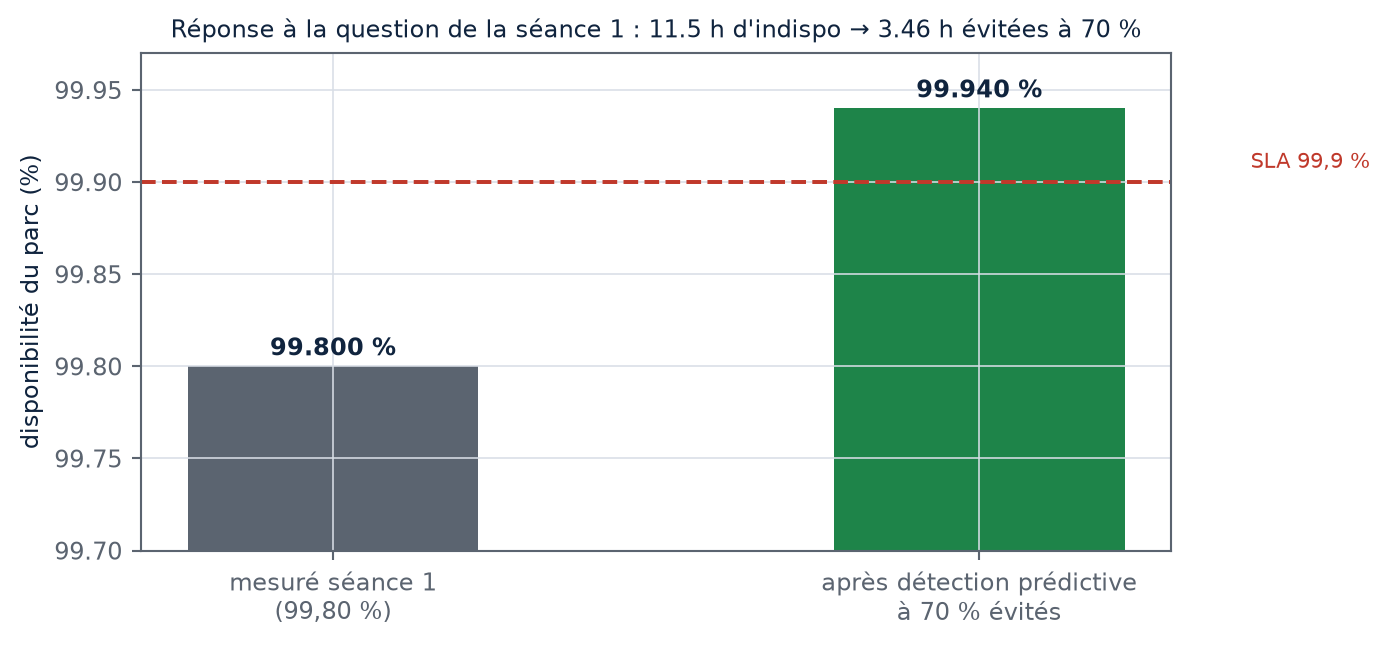
\includegraphics[width=\textwidth]{f24_dispo_predictif.png}
\end{center}
\begin{kbox}[La boucle est bouclée]
Le rappel du détecteur EST un chiffre d'ingénierie de dispo :
passer de 0 à 0,625 de rappel, c'est racheter plus de la moitié
de l'indisponibilité. La séance 4 prolonge : \textbf{prédire}
quand, pas seulement \emph{si}.
\end{kbox}
\end{column}
\end{columns}
\end{frame}

\begin{frame}{À retenir de la séance 3}
\footnotesize%
\begin{columns}[t]
\begin{column}{0.48\textwidth}
\begin{kbox}[Les 5 idées à emporter]
\begin{enumerate}
\item \textbf{Anomalie $\ne$ incident} : le non-supervisé
(IsolationForest, LOF) name le soupçon ; le supervisé décide.
\item À 0,35 \% de positifs, \textbf{l'exactitude ne veut
rien dire} (99,65 \% en ne prédisant jamais 1).
\item \textbf{Précision/rappel/F1} et courbe PR --- jamais la
ROC --- disent la vérité métier.
\item Le \textbf{seuil est un choix métier} : budget NOC,
coût FP (fatigue) vs FN (SLA).
\item \textbf{Validation temporelle obligatoire}
(\py{TimeSeriesSplit}) : KFold mélangé $=$ fuite.
\end{enumerate}
\end{kbox}
\end{column}
\begin{column}{0.48\textwidth}
\begin{block}{Le palmarès mesuré du jour (test, corrigé)}
\begin{center}\small
\begin{tabular}{@{}l c c@{}}
\toprule
 & $F_1$ & AP\\
\midrule
Gradient boosting & \textbf{0,769} & \textbf{0,63}\\
Reg. logistique & 0,12 & 0,32\\
Forêt (balanced, seuil 0,5) & 0,00 & 0,19\\
\bottomrule
\end{tabular}
\end{center}
\end{block}
\begin{wbox}[Et le rappel manquant ?]
24 incidents sur 64 non détectés au seuil optimal. Piste de la
séance 4 : prédire la trajectoire (SARIMA) et agir \emph{avant}.
\end{wbox}
\end{column}
\end{columns}
\end{frame}

\begin{frame}{Prochaine séance --- Séance 4}
\begin{columns}[t]
\begin{column}{0.48\textwidth}
\begin{kbox}[Séries temporelles et prédiction]
\begin{itemize}
\item \textbf{SARIMA} : tendance, saisonnalité journalière et
hebdomadaire de nos métriques (les \py{h\_sin}/\py{js\_sin} du
TP2 étaient la version artisanale).
\item \textbf{Prédiction de panne} : de « cette fenêtre est
anormale » à « ce serveur tombera dans N heures ».
\item \textbf{Capacité} : extrapoler la charge et dimensionner
avant la saturation.
\end{itemize}
\end{kbox}
\end{column}
\begin{column}{0.48\textwidth}
\begin{ebox}[À préparer]
\begin{itemize}
\item Rendre le TP de la séance 3 (barème : frame précédente).
\item Relire les séries de \file{nosys\_metriques.csv} :
tendance hebdo, pics de journée --- matière brute du SARIMA.
\item Gardez vos matrices de confusion : nous comparerons
« détecter » (séance 3) et « prédire » (séance 4).
\end{itemize}
\end{ebox}
\end{column}
\end{columns}
\vspace{2mm}
\begin{center}\small
\textbf{Fin de la séance 3} --- vous savez désormais faire
parler un modèle sur des données réelles, sous contrainte métier.
\end{center}
\end{frame}

% =====================================================================
%  Seance 4 -- A. garde, plan, cours 1 : series temporelles (frames 1--10)
% =====================================================================
\section{Séance 4 --- Supervision, optimisation et prédiction}
\chapterslide{Séance 4}{Supervision, optimisation et prédiction}
{4 h --- 2 h cours / 2 h TP --- Partie 4 du syllabus EPD-GIT-5534}
{\textbf{Objectifs :} lire une série temporelle de métriques (stationnarité,
ACF/PACF, test ADF) $ \bullet $ ajuster un \textbf{SARIMA} réel et mesurer
son erreur $ \bullet $ prédire la \textbf{défaillance} sans fuite temporelle
et valider par découpage strict $ \bullet \ $passer de la prévision à la
\textbf{décision} : autoscaling, saturation, disponibilité.}

\begin{frame}{Plan de la séance (4 h)}
\footnotesize%
\begin{columns}[t]
\begin{column}{0.48\textwidth}
\begin{kbox}[Cours magistral --- 2 h]
\begin{enumerate}
\item \textbf{Séries temporelles de métriques} (50 min) : stationnarité,
ADF, ACF/PACF, ARIMA/SARIMA, résidus.
\item \textbf{Prédiction de défaillance} (50 min) : horizon, étiquette,
fuite temporelle, validation temporelle stricte.
\item \textbf{Optimisation} (20 min) : prévision $\to$ marge $\to$
capacité ; autoscaling ; saturation ; disponibilité.
\end{enumerate}
\end{kbox}
\end{column}
\begin{column}{0.48\textwidth}
\begin{ebox}[Travaux pratiques --- 2 h]
\textbf{« Prévoir et décider »} sur \file{nosys\_metriques.csv} et
\file{nosys\_features.csv} :
\begin{enumerate}
\item B1 --- série horaire, décomposition, ADF (30 min)
\item B2 --- SARIMA : ajuster, prévoir, mesurer la MAE (40 min)
\item B3 --- modèle de panne, split temporel strict (30 min)
\item B4 --- rappel vs budget d'alertes (20 min)
\item B5 --- livrable : prévision + tableau + saturation (10 min)
\end{enumerate}
\end{ebox}
\end{column}
\end{columns}
\vspace{1mm}
\begin{center}\small
Nouveaux outils du dossier : \file{statsmodels} et la
\textbf{validation temporelle} --- le découpage du 22/09
remplace le KFold.
\end{center}
\end{frame}

\begin{frame}{Cours 1 --- De la métrique à la série temporelle}
\begin{columns}[t]
\begin{column}{0.52\textwidth}
\begin{block}{Ce que nous avons déjà}
Depuis la séance 2, nous savons \textbf{nettoyer} une métrique et en
extraire des \textbf{signaux} (fenêtres, p99, encodage cyclique).
\end{block}
\begin{block}{Ce qui change aujourd'hui}
On ne résume plus le passé : on le \textbf{prolonge}.
\begin{itemize}
\item Une série temporelle = observations ordonnées dans le temps,
\textbf{l'ordre porte l'information}.
\item Deux questions : à quoi ressemble la série
(\textbf{tendance} + \textbf{saison} + bruit) ? et que se passera-t-il
demain ?
\end{itemize}
\end{block}
\end{column}
\begin{column}{0.44\textwidth}
\begin{ebox}[Le série du dossier]
Agrégat \textbf{horaire} du parc : CPU moyen des 8 serveurs, du 01/09 au
30/09/2026 --- \textbf{720 points} (au lieu de 69 120 à 5 min : on
reste léger, et s = 24 au lieu de s = 288).
\end{ebox}
\begin{wbox}[Pourquoi agréger ?]
À 5 min, la saison journalière fait s = 288 : un SARIMA avec autant de
retards est coûteux et instable. L'heure garde le cycle jour/nuit ---
l'essentiel pour décider de la \textbf{capacité}.
\end{wbox}
\end{column}
\end{columns}
\end{frame}

\begin{frame}{Stationnarité : l'hypothèse qui rend le modèle possible}
\begin{columns}[t]
\begin{column}{0.5\textwidth}
\begin{block}{Définition intuitive}
Une série est \textbf{stationnaire} si ses propriétés statistiques ne
dépendent pas du moment observé :
\begin{itemize}
\item moyenne \textbf{stable} (pas de dérive) ;
\item variance stable (pas d'explosion) ;
\item autocorrélation qui ne dépend que du \textbf{décalage}, pas de la date.
\end{itemize}
Un modèle ARIMA \emph{apprend} les relations entre retards : cela n'a de
sens que si ces relations sont \textbf{les mêmes hier et demain}.
\end{block}
\end{column}
\begin{column}{0.46\textwidth}
\begin{ebox}[Sur notre série (test ADF réel)]
\footnotesize
\begin{tabular}{@{}lc@{}}
\toprule
série & $p$-value ADF\\
\midrule
brute & 0,0753\\
différenciée ($d=1$) & $\approx 0$\\
diff. saisonnière ($s=24$) & $3\times10^{-7}$\\
\bottomrule
\end{tabular}
\end{ebox}
\begin{kbox}[Lecture]
Brute : on ne peut pas rejeter la non-stationnarité à 5 \% ($p = 0{,}075$).
Après différenciation : stationnaire. \textbf{C'est le $d$ et le $D$ du
modèle.}
\end{kbox}
\end{column}
\end{columns}
\end{frame}

\begin{frame}[fragile]{Le test ADF, expliqué simplement}
\footnotesize%
\begin{columns}[t]
\begin{column}{0.52\textwidth}
\begin{block}{L'idée}
On teste l'\textbf{hypothèse nulle} : « la série possède une racine
unitaire », c'est-à-dire qu'elle est \emph{non stationnaire} (une
secousse y laisse une trace permanente).
\begin{itemize}
\item Statistique de test : régression augmentée de Dickey-Fuller
(la série sur ses propres retards).
\item $p$-value \textbf{petite} $\Rightarrow$ on rejette H0
$\Rightarrow$ série stationnaire.
\item $p$-value \textbf{grande} $\Rightarrow$ on différencie
($d = d+1$) et on recommence.
\end{itemize}
\end{block}
\end{column}
\begin{column}{0.44\textwidth}
\begin{wbox}[Le piège d'interprétation]
ADF \textbf{ne prouve pas} la stationnarité : il rejette (ou non) une
hypothèse. Série courte + saisonnalité forte $\Rightarrow$ compléter
toujours par un \textbf{regard graphique} (ACF lente = non stationnaire).
\end{wbox}
\end{column}
\end{columns}
\vspace{1mm}
\begin{codebox}[Deux lignes suffisent]
\begin{lstlisting}
from statsmodels.tsa.stattools import adfuller
stat, p, *_ = adfuller(serie)
print(p)   # 0.075 : on differencie
\end{lstlisting}
\end{codebox}
\end{frame}

\begin{frame}{ACF et PACF : la carte d'identité de la série}
\begin{center}
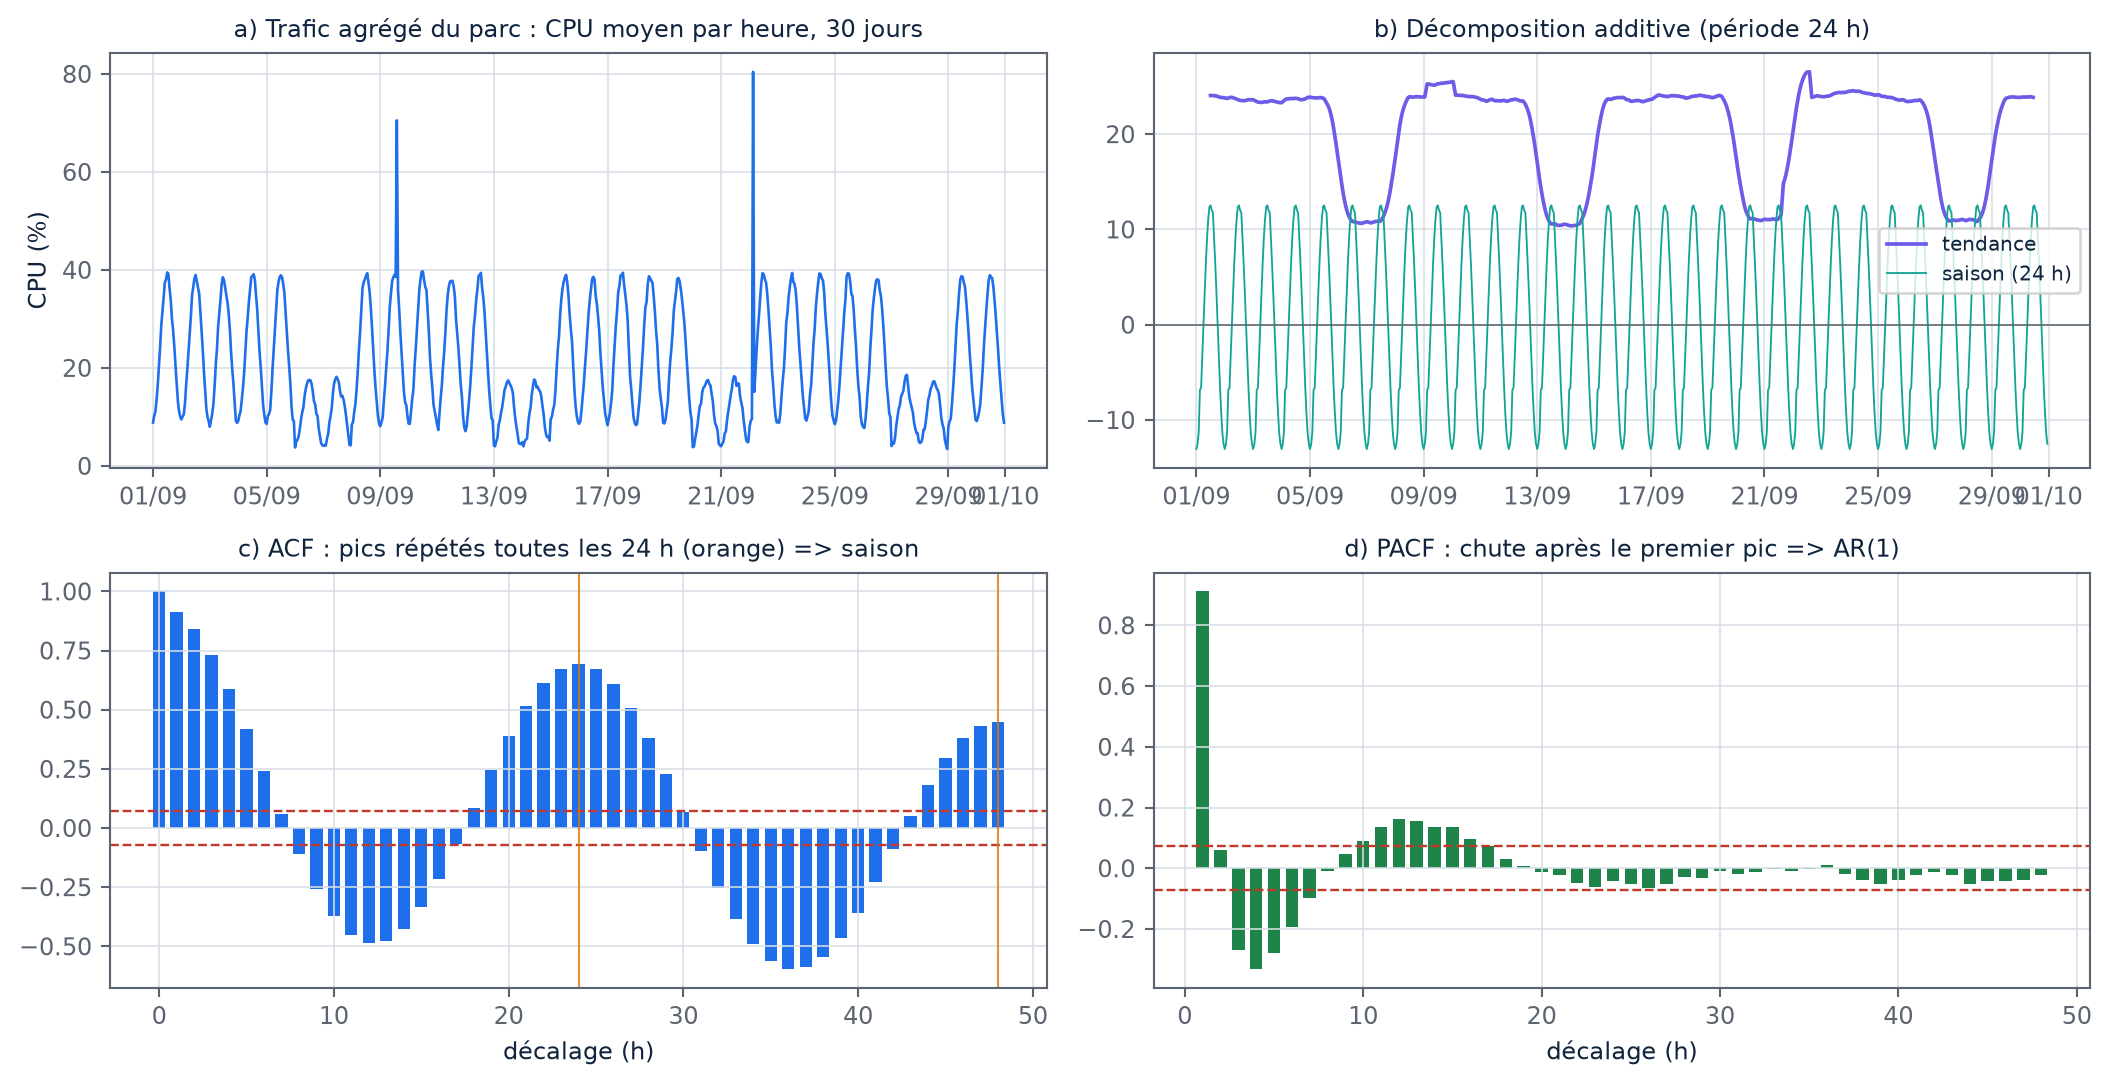
\includegraphics[width=0.82\textwidth]{f25_decomposition_acf.png}
\end{center}
\vspace{-1mm}
\begin{kbox}[Comment lire]
\small
\textbf{ACF} qui décroît lentement = non stationnarité ; pics répétés
toutes les 24 h = \textbf{saison journalière}. \textbf{PACF} qui chute
après le premier retard = \textbf{AR(1)}. Ces graphiques donnent le
premier candidat : $p$ $\approx$ retards PACF, $q$ $\approx$ retards
ACF, saison au lag 24.
\end{kbox}
\end{frame}

\begin{frame}{ARIMA : que signifient p, d, q ?}
\begin{center}\small
\begin{tabular}{@{}p{1.4cm}p{5.6cm}p{4.6cm}@{}}
\toprule
\textbf{Param.} & \textbf{Signification} & \textbf{Comment le choisir}\\
\midrule
$p$ & \textbf{AR} : régression sur les $p$ valeurs passées & retards
significatifs de la \textbf{PACF}\\
\addlinespace[1pt]
$d$ & \textbf{différenciation} : nb de fois où l'on soustrait la valeur
précédente pour stabiliser & test \textbf{ADF} (le minimum qui stationnarise)\\
\addlinespace[1pt]
$q$ & \textbf{MA} : régression sur les $q$ erreurs passées & retards
significatifs de l'\textbf{ACF}\\
\bottomrule
\end{tabular}
\end{center}
\vspace{1mm}
\begin{ebox}[Version saisonnière SARIMA$(p,d,q)(P,D,Q)_s$]
Mêmes trois nombres, appliqués au \textbf{retard saisonnier} $s$ : ici
$s = 24$ (agrégat horaire). À 5 min on aurait $s = 288$, à 15 min
$s = 96$ --- lourds : d'où notre agrégation à l'heure.
\end{ebox}
\vspace{1mm}
\begin{center}\small
Notation du dossier : SARIMA$(p,d,q)\times(P,D,Q)_{24}$ --- on choisit la
grille par \textbf{AIC} (qualité de l'ajustement pénalisée par la
complexité).
\end{center}
\end{frame}

\begin{frame}{Le SARIMA du dossier, réellement ajusté}
\begin{columns}[t]
\begin{column}{0.52\textwidth}
\begin{block}{Protocole (graine 5534, 2 threads)}
\begin{itemize}
\item entraînement : 24 premiers jours = \textbf{576 points} ;
\item grille $(p,0,q) \times (1,0,1)_{24}$, harmoniques hebdomadaires
en exogènes (la semaine se connaît d'avance, comme l'heure) ;
\item sélection par \textbf{AIC}, prévision des 6 jours suivants.
\end{itemize}
\end{block}
\begin{solbox}[Résultats mesurés]
Meilleur ordre : SARIMA$(2,0,1)\times(1,0,1)_{24}$
(AIC 3\,121,5). \textbf{MAE test = 3,01 pts CPU} contre 5,06
(persistance 24 h) et 5,23 (semaine précédente) : \textbf{$-40{,}5$ \%}
d'erreur.
\end{solbox}
\end{column}
\begin{column}{0.44\textwidth}
\begin{wbox}[Résidus : le modèle n'est pas parfait]
Ljung-Box sur les résidus (lag 24) : $p < 0{,}001$ --- il reste de
l'autocorrélation. Traduction : le SARIMA capte tendance + cycles, mais
les \textbf{incidents} (pics) échappent encore au modèle.
\footnotesize Une phrase à retenir : \emph{le test de Ljung-Box vérifie
que les résidus ne contiennent plus de structure temporelle exploitable.}
\end{wbox}
\end{column}
\end{columns}
\end{frame}

\begin{frame}{Quiz 1 --- séries temporelles (5 min)}
\begin{qbox}[3 questions]
\begin{enumerate}
\item Une série dont l'ACF décroît très lentement est probablement :\\
(a) stationnaire \quad (b) non stationnaire --- il faut différencier \quad
(c) saisonnière seulement
\item À 5 min de granularité, la saison journalière vaut :\\
(a) $s = 24$ \quad (b) $s = 96$ \quad (c) $s = 288$
\item Sur notre série, l'ADF donne $p = 0{,}075$ sur la série brute. Que
fait-on ?\\
(a) on accepte la stationnarité \quad (b) on différencie et on reteste
\quad (c) on augmente $q$
\end{enumerate}
\end{qbox}
\vspace{1mm}
\begin{solbox}[Réponses]
\textbf{1 : b} \quad \textbf{2 : c} (288 pas de 5 min par jour ; 96 à
15 min ; 24 à l'heure) \quad \textbf{3 : b} --- $p > 0{,}05$ : on ne
rejette pas H0, on différencie ($d$ ou $D$) puis on reteste.
\end{solbox}
\end{frame}

% =====================================================================
%  Seance 4 -- B. cours 2 : prediction de defaillance (frames 11--16)
% =====================================================================
\section{Cours 2 --- Prédiction de défaillance}

\begin{frame}{Cours 2 --- Prédire la panne : horizon et étiquette}
\begin{columns}[t]
\begin{column}{0.52\textwidth}
\begin{block}{L'horizon de prédiction, choisi AVANT le modèle}
\begin{itemize}
\item \textbf{« Panne dans $h$ heures »} : l'horizon $h$ n'est pas un
détail technique, c'est une \textbf{décision métier}. Trop court : le
sommaire n'a pas le temps d'agir. Trop long : la prédiction devient
bruitée.
\item Notre dossier : $h = 30$ min --- exactement l'étiquette
\py{incident_30min} construite au TP2 à partir de la colonne
\py{alarme} du \textbf{futur uniquement}.
\end{itemize}
\end{block}
\end{column}
\begin{column}{0.44\textwidth}
\begin{ebox}[Le dataset prêt]
\file{nosys\_features.csv} : 34 560 fenêtres de 10 min
(8 serveurs $\times$ 30 jours), 120 positives (0,35 \%) ;
split temporel : entraînement \textbf{avant} le 22/09 (24 192 lignes,
56 positives), test \textbf{après} (10 368 lignes, 64 positives).
\end{ebox}
\begin{kbox}[Le point de bascule]
La séance 3 détectait les \textbf{anomalies} (l'incident est en cours).
Aujourd'hui on le \textbf{précède} --- et tout change, surtout la
validation.
\end{kbox}
\end{column}
\end{columns}
\end{frame}

\begin{frame}[fragile]{Le piège n°1 : la fuite temporelle}
\footnotesize%
\begin{columns}[t]
\setlength{\columnsep}{2pt}
\begin{column}{0.50\textwidth}
\begin{lstlisting}
# FAUX : l'alarme courante dans les features
features = ["cpu_moy", "ram_moy", ..., "alarme"]
# or l'etiquette incident_30min CONTIENT
# l'alarme de la fenetre courante :
# label(t) = max(alarme t..t+30min)
\end{lstlisting}
\begin{wbox}[Ce que donne réellement cette fuite (mesuré sur le test)]
\scriptsize
\begin{tabular}{@{}lc@{}}
\toprule
 & P(incid. $\le$ 30 min)\\
\midrule
alarme courante (40 fen.) & \textbf{100 \%}\\
pas d'alarme (10 328) & 0,23 \%\\
\bottomrule
\end{tabular}
\end{wbox}
\end{column}
\begin{column}{0.44\textwidth}
\begin{block}{Pourquoi c'est grave}
\begin{itemize}
\item La variable « prédit » l'étiquette à 100 \% parce qu'elle
\textbf{est} un morceau de l'étiquette : on ne prédit plus, on
\textbf{constate} le présent.
\item En production, cette information arrive \textbf{avec} l'incident,
pas avant : le modèle « magique » devient inutile.
\item Et il reste \textbf{aveugle} aux 24 incidents sans alarme
courante : rappel plafonné à 62,5 \%.
\end{itemize}
\end{block}
\end{column}
\end{columns}
\end{frame}

\begin{frame}{Validation : découpage temporel strict, JAMAIS de shuffle}
\begin{columns}[t]
\begin{column}{0.52\textwidth}
\begin{block}{La règle du dossier}
\begin{center}
\footnotesize entraînement : \textbf{fenêtre $<$ 22/09 00:00} \quad
$\Big|$ \quad test : \textbf{fenêtre $\ge$ 22/09}
\end{center}
\begin{itemize}
\item Le futur ne sert \textbf{jamais} à entraîner : on simule la mise
en production réelle, où l'on prédit \emph{à partir d'aujourd'hui}.
\item La standardisation, les seuils, les encodages : tout se calcule
\textbf{sur le train} puis s'applique au test.
\end{itemize}
\end{block}
\end{column}
\begin{column}{0.44\textwidth}
\begin{ebox}[KFold aléatoire : mesuré sur le dossier]
\small Rappel moyen en KFold aléatoire 5 plis : \textbf{0,60}
$(0{,}54$ à $0{,}63)$ ; découpage temporel strict : \textbf{0,625}.
\end{ebox}
\begin{wbox}[KFold aléatoire : une structure fausse]
\small
Ici les chiffres sont proches --- et c'est le piège : le KFold entraîne
\textbf{sur le futur} et teste sur le passé. La structure de validation
est fausse ; dès que la série dérive (nouvelle charge, évolution du
parc), le KFold promet des performances qui n'existeront pas.
\end{wbox}
\end{column}
\end{columns}
\end{frame}

\begin{frame}{Le modèle du dossier : GradientBoostingClassifier}
\footnotesize%
\begin{columns}[t]
\begin{column}{0.5\textwidth}
\begin{block}{Réglage et protocole}
\begin{itemize}
\item 12 variables de signaux (niveaux, dispersion, latence p99,
dynamique, contexte cyclique) --- \textbf{sans} l'alarme ;
\item \py{GradientBoostingClassifier} (300 arbres, profondeur 4,
graine 5534) ;
\item split temporel strict au 22/09, seuil 0,5.
\end{itemize}
\end{block}
\begin{solbox}[Matrice de confusion test (mesurée)]
\footnotesize
\begin{tabular}{@{}lcc@{}}
\toprule
 & prédit 0 & prédit 1\\
\midrule
réel 0 & 10 290 & 14\\
réel 1 & 24 & \textbf{40}\\
\bottomrule
\end{tabular}\\[1mm]
rappel \textbf{62,5 \%} \quad précision \textbf{74,1 \%}
\end{solbox}
\end{column}
\begin{column}{0.46\textwidth}
\begin{center}
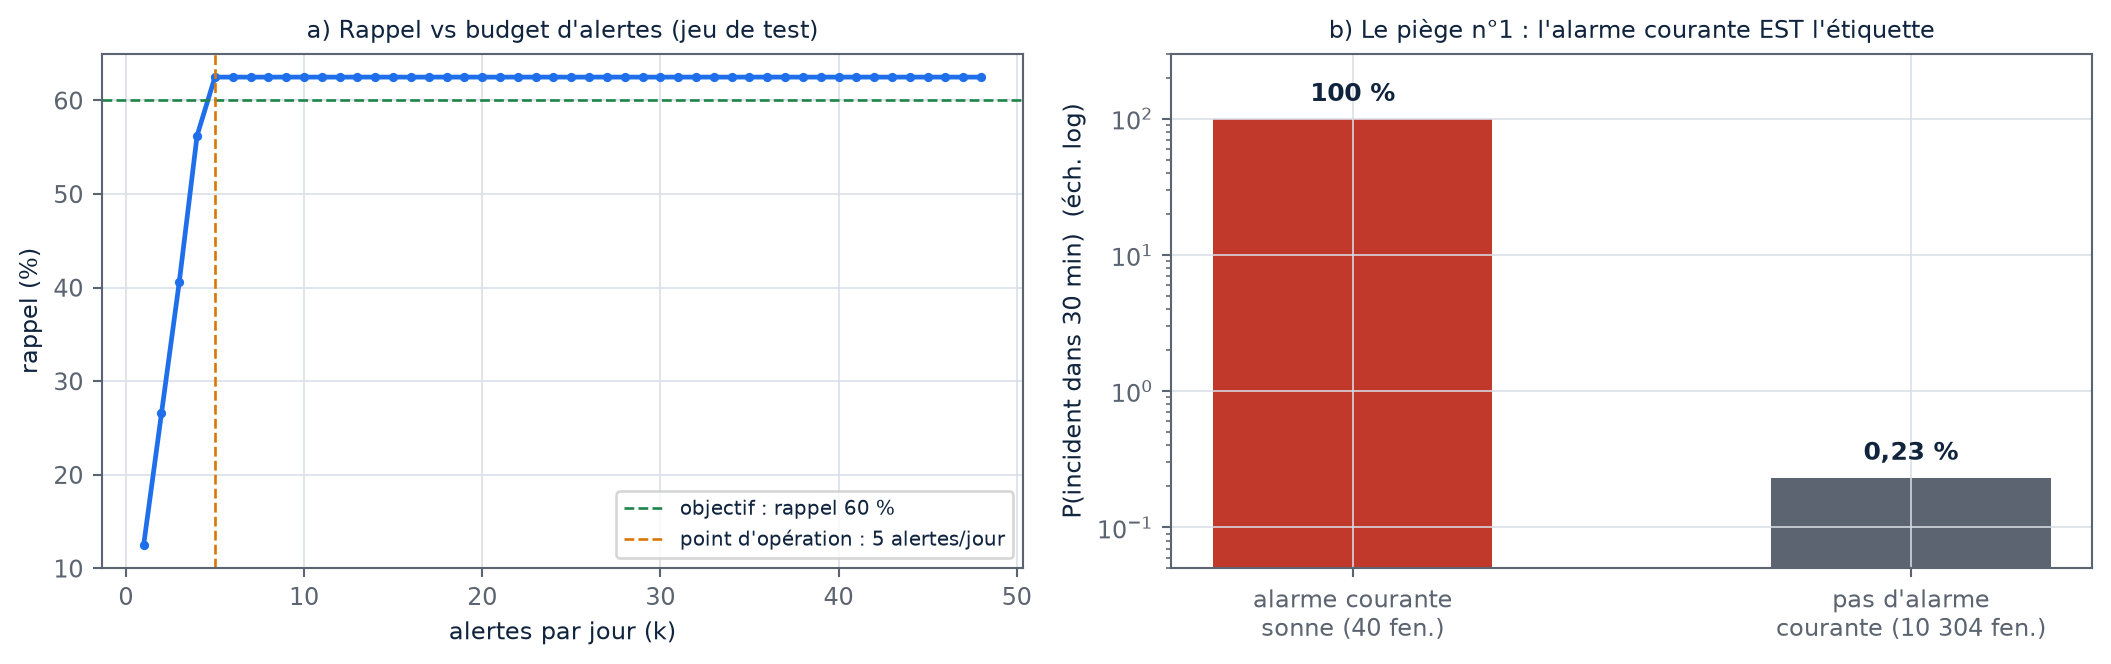
\includegraphics[width=\textwidth]{f27_rappel_alertes.png}
\end{center}
\begin{kbox}[Lecture]
Avec 5 alertes par jour, on rattrape \textbf{62,5 \%} des pannes à 30
min --- les 10 290 vrais négatifs évitent des alertes inutiles. La
limite à 62,5 \% n'est pas un mauvais réglage : 24 incidents n'ont
\textbf{aucun signal détectable} dans les métriques seules.
\end{kbox}
\end{column}
\end{columns}
\end{frame}

\begin{frame}{Quiz 2 --- prédiction de défaillance (5 min)}
\begin{qbox}[3 questions]
\begin{enumerate}
\item On ajoute l'alarme courante aux variables d'entrée. Sur le jeu de
test, la précision paraît excellente. Le vrai problème :\\
(a) le modèle est trop lent \quad (b) l'alarme \textbf{est} un morceau
de l'étiquette : on constate au lieu de prédire \quad (c) il manque des
données
\item Le bon découpage pour ce dataset est :\\
(a) 80/20 au hasard \quad (b) entraîner avant le 22/09, tester après
\quad (c) KFold aléatoire 5 plis
\item Avec 5 alertes par jour au point d'opération, le rappel mesuré est :\\
(a) 25 \% \quad (b) 62,5 \% \quad (c) 100 \%
\end{enumerate}
\end{qbox}
\vspace{1mm}
\begin{solbox}[Réponses]
\textbf{1 : b} --- fuite temporelle ; l'alarme sonne \emph{avec}
l'incident, jamais avant. \quad \textbf{2 : b} --- le temps ne se
mélange pas. \quad \textbf{3 : b} --- 40 pannes rattrapées sur 64.
\end{solbox}
\end{frame}

% =====================================================================
%  Seance 4 -- C. cours 3 : optimisation + reponse seance 1 (frames 17--21)
% =====================================================================
\section{Cours 3 --- De la prévision à la décision}

\begin{frame}{Cours 3 --- La chaîne prévision $\to$ marge $\to$ capacité}
\footnotesize%
\begin{center}
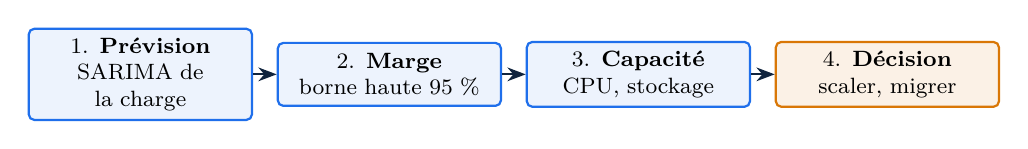
\begin{tikzpicture}[node distance=4mm,
  b/.style={draw=byBlue,thick,rounded corners=2pt,fill=byBlue!8,
            minimum height=8mm,text width=2.6cm,align=center,font=\footnotesize},
  a/.style={draw=byOrange,thick,rounded corners=2pt,fill=byOrange!10,
            minimum height=8mm,text width=2.6cm,align=center,font=\footnotesize}]
\node[b] (p) {1. \textbf{Prévision}\\ SARIMA de la charge};
\node[b,right=3mm of p] (m) {2. \textbf{Marge}\\ borne haute 95 \%};
\node[b,right=3mm of m] (c) {3. \textbf{Capacité}\\ CPU, stockage};
\node[a,right=3mm of c] (d) {4. \textbf{Décision}\\ scaler, migrer};
\draw[-{Stealth},thick,byDeep] (p) -- (m);
\draw[-{Stealth},thick,byDeep] (m) -- (c);
\draw[-{Stealth},thick,byDeep] (c) -- (d);
\end{tikzpicture}
\end{center}
\vspace{1mm}
\begin{block}{L'idée clé}
Une prévision \textbf{sans intervalle} ne suffit pas pour dimensionner :
on utilise la \textbf{borne haute} de l'intervalle de confiance (95 \%)
comme marge de sécurité. La MAE mesurée (3,01 pts CPU) dit à quel point
la marge peut être serrée.
\end{block}
\vspace{1mm}
\begin{ebox}[Exemple concret sur le dossier]
Prévision du pic de demain : $p$ pts CPU $\pm$ intervalle. Capacité d'un
serveur : 100 pts. Si la borne haute dépasse la capacité agrégée
$\Rightarrow$ ajouter une instance \textbf{avant} le pic, pas pendant.
\end{ebox}
\end{frame}

\begin{frame}{Autoscaling : décider sans humain dans la boucle}
\begin{columns}[t]
\begin{column}{0.52\textwidth}
\begin{block}{Deux familles de règles}
\begin{itemize}
\item \textbf{Réactif} : seuil observé (CPU $>$ 80 \% pendant 10 min)
$\Rightarrow$ scaler. Simple, mais \textbf{en retard} sur un pic rapide.
\item \textbf{Prédictif} : la prévision SARIMA anticipe le pic de la
période de charge (notre CPU jour 30,2 \% / nuit 10,0 \%) et scale
\textbf{avant}.
\end{itemize}
\end{block}
\begin{kbox}[Où le ML entre]
Le modèle donne la \textbf{trajectoire} (forme + intervalle) ; la
politique de scaling combine prévision + coût : scaler trop tôt coûte
de l'argent inutile, trop tard coûte des incidents --- exactement
l'arbitrage précision/rappel du cours 2.
\end{kbox}
\end{column}
\begin{column}{0.44\textwidth}
\begin{wbox}[Garde-fous obligatoires]
\begin{itemize}
\item Cooldown : ne pas scaler deux fois en 10 min.
\item Bornes min/max d'instances.
\item Journaliser chaque décision : un autoscaler est lui-même un
système à superviser.
\end{itemize}
\end{wbox}
\end{column}
\end{columns}
\end{frame}

\begin{frame}{Date de saturation du stockage : un calcul réel}
\begin{center}
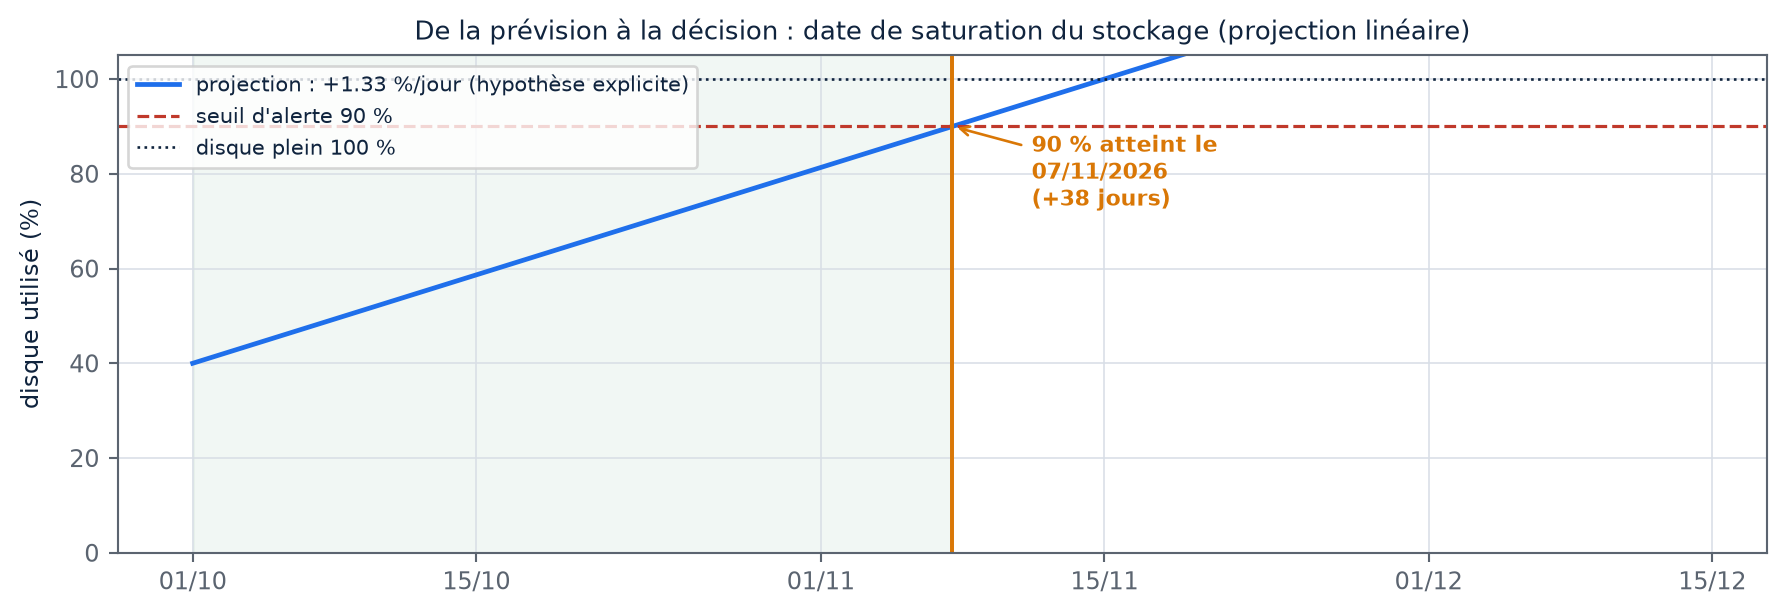
\includegraphics[width=0.88\textwidth]{f28_saturation.png}
\end{center}
\vspace{-1mm}
\begin{columns}[t]
\begin{column}{0.52\textwidth}
\begin{block}{Hypothèses explicites}
\small Métriques + logs : 40 \% du disque après 30 jours de rétention
$\Rightarrow$ \textbf{+1,33 \%/jour} ; seuil d'alerte 90 \%.
\end{block}
\end{column}
\begin{column}{0.44\textwidth}
\begin{solbox}[Calcul]
\small $(90-40)/1{,}333 = 37{,}5$ jours $\Rightarrow$ 90 \% atteint le
\textbf{07/11/2026} ; disque plein début décembre.
\end{solbox}
\end{column}
\end{columns}
\end{frame}

\begin{frame}{La réponse à la question de la séance 1}
\begin{qbox}[La question laissée ouverte en séance 1]
\begin{center}\normalsize
« Si on détectait 70 \% des incidents 30 minutes à l'avance,\\
quelle disponibilité atteindrions-nous ? »
\end{center}
\end{qbox}
\vspace{1mm}
\begin{columns}[t]
\begin{column}{0.52\textwidth}
\begin{block}{Le raisonnement (chiffres du dossier)}
\begin{itemize}
\item indisponibilité cumulée mesurée (séance 1) : \textbf{11,3 h} ;
\item 70 \% évités $\Rightarrow$ indispo restante
$11{,}3 \times 0{,}3 = \mathbf{3{,}39}$ h ;
\item fenêtre de mesure du dossier : $8$ serveurs $\times\ 720$ h
$=$ \textbf{5 760 heures-serveur}.
\end{itemize}
\end{block}
\end{column}
\begin{column}{0.44\textwidth}
\begin{solbox}[Le résultat officiel]
\begin{center}
$\text{dispo} = 1 - \dfrac{3{,}39}{5\,760} = \mathbf{99{,}941\ \%}$
\end{center}
\vspace{1mm}
\textbf{$>$ SLA 99,9 \%} : la détection prédictive n'est pas un
gadget, elle fait \textbf{basculer le parc au-dessus du SLA} --- c'est
la promesse tenue par la partie 4 du syllabus.
\end{solbox}
\end{column}
\end{columns}
\end{frame}

\begin{frame}{Quiz 3 --- optimisation (5 min)}
\begin{qbox}[3 questions]
\begin{enumerate}
\item Pour dimensionner la capacité, on utilise :\\
(a) la moyenne de la prévision \quad (b) la borne haute de l'intervalle
de confiance \quad (c) le maximum historique
\item Le scaling \textbf{prédictif} différend du réactif car :\\
(a) il est gratuit \quad (b) il agit \emph{avant} le pic grâce à la
prévision \quad (c) il ne peut pas se tromper
\item Avec +1,33 \%/jour et 40 \% utilisés, le seuil 90 \% est atteint :\\
(a) après 37,5 jours \quad (b) après 90 jours \quad (c) jamais
\end{enumerate}
\end{qbox}
\vspace{1mm}
\begin{solbox}[Réponses]
\textbf{1 : b} --- la marge vient de l'incertitude mesurée.
\quad \textbf{2 : b} --- et il peut se tromper : d'où les garde-fous.
\quad \textbf{3 : a} --- 50 points à 1,33 point/jour, soit le
07/11/2026.
\end{solbox}
\end{frame}

% =====================================================================
%  Seance 4 -- D. TP : prevoir et decider (frames 22--27)
% =====================================================================
\section{TP « Prévoir et décider »}

\begin{frame}[fragile]{TP B1 --- la série horaire du parc (30 min)}
\begin{codebox}[B1. Agréger, décomposer, tester]
\begin{lstlisting}
import pandas as pd
from statsmodels.tsa.seasonal import seasonal_decompose
from statsmodels.tsa.stattools import adfuller

m = pd.read_csv("data/nosys_metriques.csv",
                parse_dates=["horodatage"])
s = m.set_index("horodatage")["cpu_pct"].resample("1h").mean()
print(len(s))                     # 720

dec = seasonal_decompose(s, model="additive", period=24)
dec.plot()                        # tendance + saison + residus

stat, p, *_ = adfuller(s)         # 0.075 : on differencie
stat, p, *_ = adfuller((s - s.shift(24)).dropna())  # ~0
\end{lstlisting}
\end{codebox}
\begin{abox}[Livrable B1]
Un graphique à 4 panneaux : série, décomposition, ACF, PACF
(\py{plot_acf}, \py{plot_pacf} de \py{statsmodels}) + la conclusion
ADF en une phrase. Vos chiffres doivent retrouver ceux du cours :
$p_{\text{brut}} = 0{,}075$, saison à 24 h.
\end{abox}
\end{frame}

\begin{frame}[fragile]{TP B2 --- SARIMA : ajuster, prévoir, mesurer (40 min)}
\begin{codebox}[B2. Le protocole du cours, exécuté par vous]
\begin{lstlisting}
from statsmodels.tsa.statespace.sarimax import SARIMAX
import numpy as np

train, test = s.iloc[:576], s.iloc[576:]
t = np.arange(len(s))             # harmoniques hebdo (exogenes)
X = np.column_stack(
    [f(t*2*np.pi*j/168) for j in (1,2,3)
     for f in (np.sin, np.cos)])

mod = SARIMAX(train, exog=X[:576],
              order=(2,0,1), seasonal_order=(1,0,1,24))
res = mod.fit(disp=False)
fc = res.get_forecast(144, exog=X[576:])
pred, ci = fc.predicted_mean, fc.conf_int()

mae = np.mean(np.abs(pred - test))     # ~3.0
\end{lstlisting}
\end{codebox}
\begin{wbox}[Deux contrôles obligatoires]
\begin{enumerate}
\item MAE \textbf{mesurée} sur les 144 heures de test, jamais sur le
train --- et comparée à deux bases naïves (persistance 24 h : 5,06 ;
semaine précédente : 5,23).
\item Toujours tracer \textbf{l'intervalle} : c'est lui qui porte la
marge de capacité du cours 3.
\end{enumerate}
\end{wbox}
\end{frame}

\begin{frame}{B2 --- ce que vous devez observer}
\begin{center}
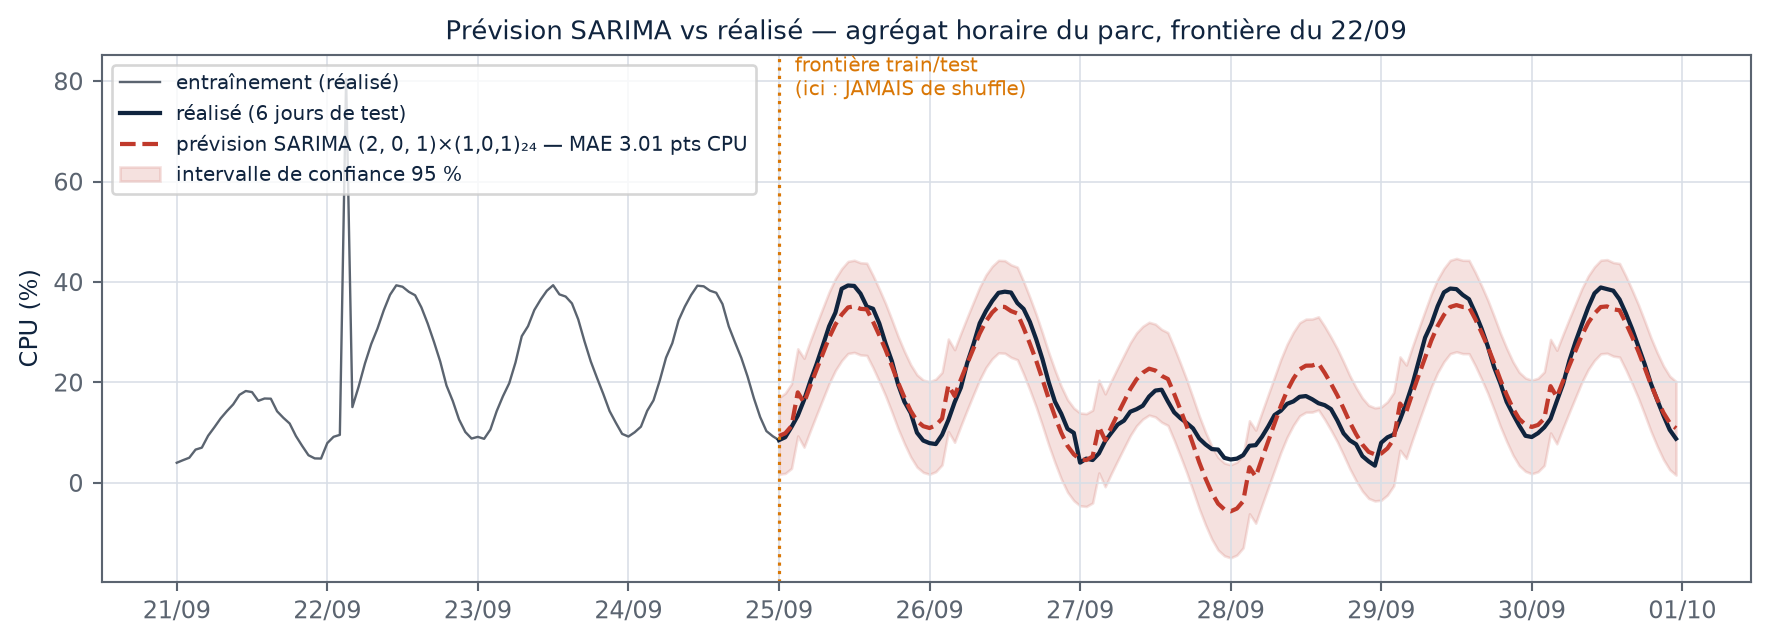
\includegraphics[width=0.8\textwidth]{f26_sarima_prevision.png}
\end{center}
\vspace{1mm}
\begin{columns}[t]
\begin{column}{0.5\textwidth}
\begin{solbox}[Résultat de référence]
\small
MAE test \textbf{3,01 pts CPU} : \textbf{$-40{,}5$ \%} d'erreur par
rapport à la persistance. L'intervalle 95 \% couvre l'essentiel des
pics --- sauf les incidents, invisibles pour un modèle de niveau.
\end{solbox}
\end{column}
\begin{column}{0.46\textwidth}
\begin{qbox}[Question d'analyse]
\small
Pourquoi l'intervalle s'élargit-il avec l'horizon ? (réponse :
l'incertitude de prévision s'accumule --- au-delà de quelques jours,
prévoir et moyenne hebdomadaire se valent.)
\end{qbox}
\end{column}
\end{columns}
\end{frame}

\begin{frame}[fragile]{TP B3 --- modèle de panne, split temporel strict (30 min)}
\footnotesize%
\begin{codebox}[B3. Le split qui respecte le temps]
\begin{lstlisting}
from sklearn.ensemble import GradientBoostingClassifier
from sklearn.metrics import confusion_matrix

f = pd.read_csv("data/nosys_features.csv",
                parse_dates=["fenetre"])
feats = ["cpu_moy","cpu_max","ram_moy","lat_moy","lat_p99",
         "perte_moy","temp_moy","conso_moy","cpu_delta",
         "cpu_amplitude","h_sin","h_cos"]
f = f.dropna(subset=feats+["incident_30min"])

cut = pd.Timestamp("2026-09-22")        # JAMAIS de shuffle
tr, te = f[f.fenetre < cut], f[f.fenetre >= cut]
gbc = GradientBoostingClassifier(
    n_estimators=300, max_depth=4,
    learning_rate=0.06, random_state=5534)
gbc.fit(tr[feats], tr.incident_30min)
print(confusion_matrix(te.incident_30min,
      gbc.predict(te[feats])))
# -> [[10290, 14], [24, 40]] : rappel 62,5 %
\end{lstlisting}
\end{codebox}
\begin{abox}[Vérification anti-fuite]
Refaire le modèle avec \py{alarme} en entrée : 40 fenêtres d'alarme
donnent 40 incidents « prédits » à 100 \%. C'est le signe de la fuite
--- la variable répète l'étiquette au lieu de la précéder.
\end{abox}
\end{frame}

\begin{frame}{TP B4 --- le budget d'alertes (20 min)}
\begin{columns}[t]
\begin{column}{0.52\textwidth}
\begin{block}{Principe}
Le rappel seul ne décide rien : chaque fausse alerte coûte du temps
d'astreinte. On trace le \textbf{rappel en fonction du nombre
d'alertes par jour} (classer les fenêtres de test par score
décroissant, regarder les $k$ premières chaque jour) et on choisit le
\textbf{point d'opération}.
\end{block}
\begin{solbox}[Référence du dossier]
\textbf{5 alertes/jour} $\Rightarrow$ rappel \textbf{62,5 \%}
(40 pannes sur 64 rattrapées). Au-delà, la courbe plafonne : les
24 incidents restants n'ont aucun signal métrique --- il faudra les
journaux (séance 5).
\end{solbox}
\end{column}
\begin{column}{0.44\textwidth}
\begin{qbox}[À débattre en binôme]
Votre équipe accepte 2 alertes/jour maximum. Quel rappel obtenez-vous ?
Quel compromis proposeriez-vous au responsable d'exploitation, chiffré
en incidents manqués et en heures d'astreinte ?
\end{qbox}
\end{column}
\end{columns}
\end{frame}

\begin{frame}{TP B5 --- livrable et barème}
\begin{columns}[t]
\begin{column}{0.52\textwidth}
\begin{abox}[À rendre]
\begin{enumerate}
\item \textbf{Graphique prévision/réalisé} avec intervalle (B2).
\item \textbf{Tableau rappel / alertes par jour} (B4) avec le point
d'opération choisi et justifié.
\item \textbf{Date de saturation} du stockage, avec hypothèses
explicites (cours 3).
\item \textbf{Un paragraphe} : « que décide l'exploitant lundi matin ? »
--- scale, marge, rétention, seuils.
\end{enumerate}
\end{abox}
\end{column}
\begin{column}{0.44\textwidth}
\begin{kbox}[Barème (20 pts)]
\begin{itemize}
\item B1 série, décomposition, ADF --- 4 pts
\item B2 SARIMA ajusté + MAE honnête --- \textbf{5 pts}
\item B3 modèle sans fuite + split strict --- \textbf{5 pts}
\item B4 courbe et choix du point --- 3 pts
\item B5 livrable et décision argumentée --- 3 pts
\end{itemize}
\end{kbox}
\end{column}
\end{columns}
\end{frame}

% =====================================================================
%  Seance 4 -- E. synthese, corriges, preview (frames 28--30)
% =====================================================================
\section{Synthèse}

\begin{frame}{Quiz de synthèse --- 5 questions (10 min)}
\begin{qbox}[Répondez seul(e), puis correction]
\begin{enumerate}
\item L'ACF montre des pics toutes les 24 h. Le paramètre concerné est :\\
(a) $p$ \quad (b) le terme \textbf{saisonnier} $P,Q$ avec $s=24$ \quad
(c) $d$
\item Sur la série brute, l'ADF renvoie $p = 0{,}075$. Conclusion :\\
(a) série stationnaire \quad (b) on différencie puis on reteste \quad
(c) le modèle SARIMA est inutile
\item Le MAE du SARIMA du dossier (3,01) est mesurée :\\
(a) sur le train \quad (b) sur les 144 heures de test après la
frontière du 22/09 \quad (c) par KFold aléatoire
\item L'alarme courante en variable d'entrée donne un modèle :\\
(a) meilleur, il faut l'ajouter \quad (b) en fuite : elle est un
morceau de l'étiquette \quad (c) équivalent
\item 70 \% des incidents évités 30 min à l'avance donnent une
disponibilité de :\\
(a) 99,80 \% \quad (b) 99,9 \% \quad (c) \textbf{99,941 \%}
\end{enumerate}
\end{qbox}
\end{frame}

\begin{frame}{Corrigé du quiz de synthèse}
\begin{solbox}[Réponses justifiées]
\begin{enumerate}
\item \textbf{b} --- la saison journalière se modélise par les termes
$(P,D,Q)_{s}$ ; ici $s = 24$ sur l'agrégat horaire.
\item \textbf{b} --- $p > 0{,}05$ : on ne rejette pas la racine
unitaire ; après différenciation $p \approx 0$ (mesuré :
$3\times10^{-7}$ pour $s = 24$).
\item \textbf{b} --- une MAE mesurée sur le train ou par KFold ne vaut
rien ; seule compte la prévision sur une période \emph{postérieure}
jamais vue.
\item \textbf{b} --- mesuré : alarme sonne $\Rightarrow$ 100 \% des
étiquettes à 1 ; c'est de la circularité, pas de la prédiction.
\item \textbf{c} --- $1 - 3{,}39/5\,760 = 99{,}941\ \% >$ SLA 99,9 \% :
l'argument économique du cours tient sur les chiffres réels du dossier.
\end{enumerate}
\end{solbox}
\end{frame}

\begin{frame}{À retenir et prochaine séance}
\begin{columns}[t]
\begin{column}{0.52\textwidth}
\begin{kbox}[Les 4 idées de la séance]
\begin{enumerate}
\item Stationnarité d'abord : ADF + ACF/PACF dictent $(p,d,q)$ et
$(P,D,Q)_s$ --- et l'agrégat horaire ($s=24$) garde le modèle léger.
\item Un SARIMA se juge sur sa \textbf{MAE hors échantillon} et son
intervalle --- jamais sur son train.
\item Prédire la panne = horloge stricte : étiquette future, features
passées, \textbf{split temporel}, zéro fuite.
\item La prévision devient \textbf{décision} : marge, autoscaling,
saturation --- et disponibilité chiffrée (99,941 \%).
\end{enumerate}
\end{kbox}
\end{column}
\begin{column}{0.44\textwidth}
\begin{ebox}[Preview séance 5]
\textbf{Sécurité, journaux et intrusion} : les 24 incidents sans
signal métrique ont peut-être une trace dans \file{nosys\_logs.csv} ---
analyse de logs, détection d'intrusion, corrélation métriques/événements.
Apportez votre livrable B5 : il contient les incidents que les
métriques n'expliquent pas.
\end{ebox}
\end{column}
\end{columns}
\end{frame}

% =====================================================================
%  Seance 5 -- A. menaces, telemetrie, regles vs modeles (frames 1--6)
% =====================================================================
\section{Séance 5 --- Sécurité et fiabilité des infrastructures assistées par l'IA}
\chapterslide{Séance 5}{Sécurité et fiabilité des infrastructures assistées par l'IA}
{4 h --- 2 h cours / 2 h TP --- Partie 5 du syllabus EPD-GIT-5534}
{\textbf{Objectifs :} reconnaître les grandes familles de menaces (balayage,
brute force, exfiltration, comptes compromis) et leur télémétrie $\bullet$
construire des \textbf{sessions} (machine $\times$ fenêtre) et des
\textbf{features d'attaque} depuis des logs bruts $\bullet$ détecter une
intrusion réelle par \textbf{IsolationForest} puis par une forêt supervisée
$\bullet$ mesurer précision@N, précision/rappel $\bullet$ connaître les
\textbf{limites} : attaques adversariales, fatigue d'alerte, explicabilité,
vie privée.}

\begin{frame}{Plan de la séance (4 h)}
\begin{columns}[t]
\begin{column}{0.48\textwidth}
\begin{kbox}[Cours magistral --- 2 h]
\begin{enumerate}
\item \textbf{Les menaces et leur télémétrie} (25 min) : balayage, brute force,
exfiltration, comptes compromis ; logs d'auth, netflow, EDR.
\item \textbf{Règles vs modèles} (25 min) : ce que chacun voit, ce que
chacun rate.
\item \textbf{Détecter par ML} (60 min) : sessions, features d'attaque,
IsolationForest, clustering, supervisé quand on a des étiquettes.
\item \textbf{Fiabilité du détecteur} (20 min) : dérive de modèle, qualité des
données, redondance.
\item \textbf{Limites} (30 min) : adversarial, fatigue d'alerte, SHAP, vie privée.
\end{enumerate}
\end{kbox}
\end{column}
\begin{column}{0.48\textwidth}
\begin{ebox}[Travaux pratiques --- 2 h]
\textbf{« Détecter l'intrusion de NOSYS »} sur \file{nosys\_logs.csv}
(100\,000 lignes, 7 jours) :
\begin{enumerate}
\item B1 --- parser et agréger par (machine, 10 min) (30 min)
\item B2 --- features d'attaque + entropie de Shannon (30 min)
\item B3 --- IsolationForest, top 30, précision@30 (30 min)
\item B4 --- forêt supervisée : précision / rappel (20 min)
\item B5 --- livrable : sessions suspectes + note d'incident (10 min)
\end{enumerate}
\end{ebox}
\end{column}
\end{columns}
\vspace{1mm}
\begin{center}\small
Le fil rouge : \textbf{l'intrusion brute force réelle} enfouie dans les logs
de NOSYS --- le TP la détecte \emph{de bout en bout}, avec des chiffres mesurés.
\end{center}
\end{frame}

\begin{frame}{Les quatre familles de menaces vues depuis les logs}
\begin{center}
\footnotesize
\begin{tabular}{@{}p{2.5cm}p{4.3cm}p{2.7cm}@{}}
\toprule
\textbf{Menace} & \textbf{Signature dans les données} & \textbf{Télémétrie qui la voit}\\
\midrule
\textbf{Balayage} (scan de ports, de services) & beaucoup de cibles, peu
d'événements par cible ; connexions courtes & netflow, pare-feu\\
\addlinespace[1pt]
\textbf{Brute force} & \textbf{rafales d'échecs} sur \emph{une} cible,
comptes testés en série, la nuit & logs d'auth (SSH, VPN, BDD)\\
\addlinespace[1pt]
\textbf{Exfiltration} & volume sortant anormal, transferts lents et réguliers,
heures creuses & netflow, proxy, DNS\\
\addlinespace[1pt]
\textbf{Compte compromis} & connexion \emph{réussie} mais horaire, machine ou
comportement inhabituels & logs d'auth + EDR (processus)\\
\bottomrule
\end{tabular}
\end{center}
\vspace{1mm}
\begin{kbox}[Notre cas d'école]
Dans \file{nosys\_logs.csv} : une \textbf{brute force} sur \py{bdd-principal}
dans la nuit du 05/10, 02 h -- 04 h. \py{root}, \py{admin}, \py{inconnu-*}
testés en rafale. Séance 1 l'avait \emph{annoncée} ; aujourd'hui on la
\textbf{détecte automatiquement}.
\end{kbox}
\end{frame}

\begin{frame}{La télémétrie de sécurité : trois sources, trois angles morts}
\begin{columns}[t]
\begin{column}{0.5\textwidth}
\begin{block}{Logs d'authentification}
Qui tente quoi, quand, avec quel résultat. \textbf{Notre source du jour} :
\file{nosys\_logs.csv} --- horodatage, machine, niveau, utilisateur, message,
\py{auth\_reussie}.
\begin{itemize}
\item Voit : échecs, comptes testés, rythme, horaire.
\item Rate : le trafic réseau, les process malveillants.
\end{itemize}
\end{block}
\begin{block}{Netflow / pare-feu}
Qui parle à qui, combien d'octets. Voit le balayage et l'exfiltration ;
rate le contenu et l'identité.
\end{block}
\end{column}
\begin{column}{0.46\textwidth}
\begin{block}{EDR (endpoint)}
Processus, injections, exécutions suspectes sur l'hôte. Voit le post-exploitation ;
 coûte cher en agents et en bruit.
\end{block}
\begin{wbox}[Le piège du « tout-logs »]
Nos logs contiennent \textbf{100\,000 lignes sur 7 jours} : beaucoup sont du
bruit opérationnel (rotations, sauvegardes, retries). \textbf{Personne ne les
lit à la main} --- c'est exactement le travail d'un modèle : séparer le
\emph{normal} de l'\emph{anormal}.
\end{wbox}
\end{column}
\end{columns}
\end{frame}

\begin{frame}{Règles vs modèles : ce que chacun voit}
\footnotesize%
\begin{columns}[t]
\begin{column}{0.5\textwidth}
\begin{block}{La règle : « alerte si $\ge$ 5 échecs en 10 min »}
\begin{itemize}
\item \ok{} \textbf{Explicable} : l'alerte cite sa condition.
\item \ok{} Zéro entraînement, déployable en une heure.
\item \nok{} \textbf{Trivial à contourner} : l'attaquant ralentit à
4 échecs / 10 min (l'attaque dure plus, passe inaperçue).
\item \nok{} Aveugle aux formes lentes (\emph{low and slow}).
\end{itemize}
\end{block}
\begin{ebox}[Ce que la règle trouve déjà dans nos logs]
Seuil à 5 échecs / 10 min : toutes les sessions d'attaque (12) sonnent...
et \textbf{0 session normale ne sonne} (max mesuré : 4 échecs). Sur CE jeu,
la règle suffit --- parce que l'attaque est grossière.
\end{ebox}
\end{column}
\begin{column}{0.46\textwidth}
\begin{block}{Le modèle : apprend la forme du normal}
\begin{itemize}
\item \ok{} Combine \textbf{plusieurs} dimensions faibles une à une
(échecs, comptes, entropie, nuit).
\item \ok{} Détecte des attaques \emph{sous} le seuil des règles.
\item \nok{} Nécessite des données propres et un suivi (dérive, séance 5 c).
\item \nok{} Moins explicable --- d'où SHAP (slide limites).
\end{itemize}
\end{block}
\begin{kbox}[La bonne réponse opérationnelle]
\textbf{Les deux en parallèle} : la règle protège le cas grossier et sert de
garde-fou ; le modèle attrape ce que la règle ne formule pas. On y revient en
fiabilité (cours 3).
\end{kbox}
\end{column}
\end{columns}
\end{frame}

\begin{frame}{Quiz 1 --- menaces et télémétrie (5 min)}
\begin{qbox}[3 questions]
\begin{enumerate}
\item Un attaquant teste 40 mots de passe sur \py{bdd-principal} à raison de
4 échecs toutes les 10 minutes. La règle « 5 échecs / 10 min » :\\
(a) alerte immédiatement \quad (b) ne sonne jamais --- l'attaque est sous le seuil \quad
(c) alerte à la fin
\item Quelle source voit le mieux une \textbf{exfiltration} de données ?\\
(a) les logs d'auth \quad (b) le netflow / proxy \quad (c) les tickets
\item Sur nos logs, le seuil « 5 échecs / 10 min » produit :\\
(a) des faux positifs massifs \quad (b) 12 alertes, toutes vraies, mais ne
verrait rien si l'attaque ralentissait \quad (c) rien du tout
\end{enumerate}
\end{qbox}
\vspace{1mm}
\begin{solbox}[Réponses]
\textbf{1 : b} --- c'est le scénario \emph{low and slow}, la faille des règles.
\quad
\textbf{2 : b} --- l'exfiltration est un phénomène de \emph{volume réseau}.
\quad
\textbf{3 : b} --- la règle marche aujourd'hui, mais elle est fragile.
\end{solbox}
\end{frame}

% =====================================================================
%  Seance 5 -- B. detecter par ML : sessions, features, IsolationForest
% =====================================================================
\section{Détecter par apprentissage automatique}

\begin{frame}{Étape 1 : transformer 100 000 lignes en sessions}
\footnotesize%
\begin{columns}[t]
\begin{column}{0.52\textwidth}
\begin{kbox}[Session = (machine, fenêtre de 10 min)]
\begin{itemize}
\item \py{fenetre = horodatage.dt.floor("10min")} puis
\py{groupby(["machine","fenetre"])}.
\item 100\,000 lignes $\rightarrow$ \textbf{10\,000 sessions}
(10 machines $\times$ 1\,008 fenêtres sur 7 j).
\item Une session est la bonne granularité : ni l'événement (trop bruité),
ni le serveur-jour (trop grossier).
\end{itemize}
\end{kbox}
\begin{ebox}[Chiffres mesurés sur nos logs]
\begin{itemize}
\item 4\,828 échecs sur 7 j, soit $\approx$ \textbf{690 / jour} --- la mesure
corrige le « $\sim$30 / jour » de la séance 1.
\item \textbf{12 sessions d'attaque} (bdd-principal, 02 h--04 h le 05/10)
sur 10\,000 : \textbf{0,12 \%} --- l'aiguille du SOC.
\end{itemize}
\end{ebox}
\end{column}
\begin{column}{0.44\textwidth}
\begin{center}
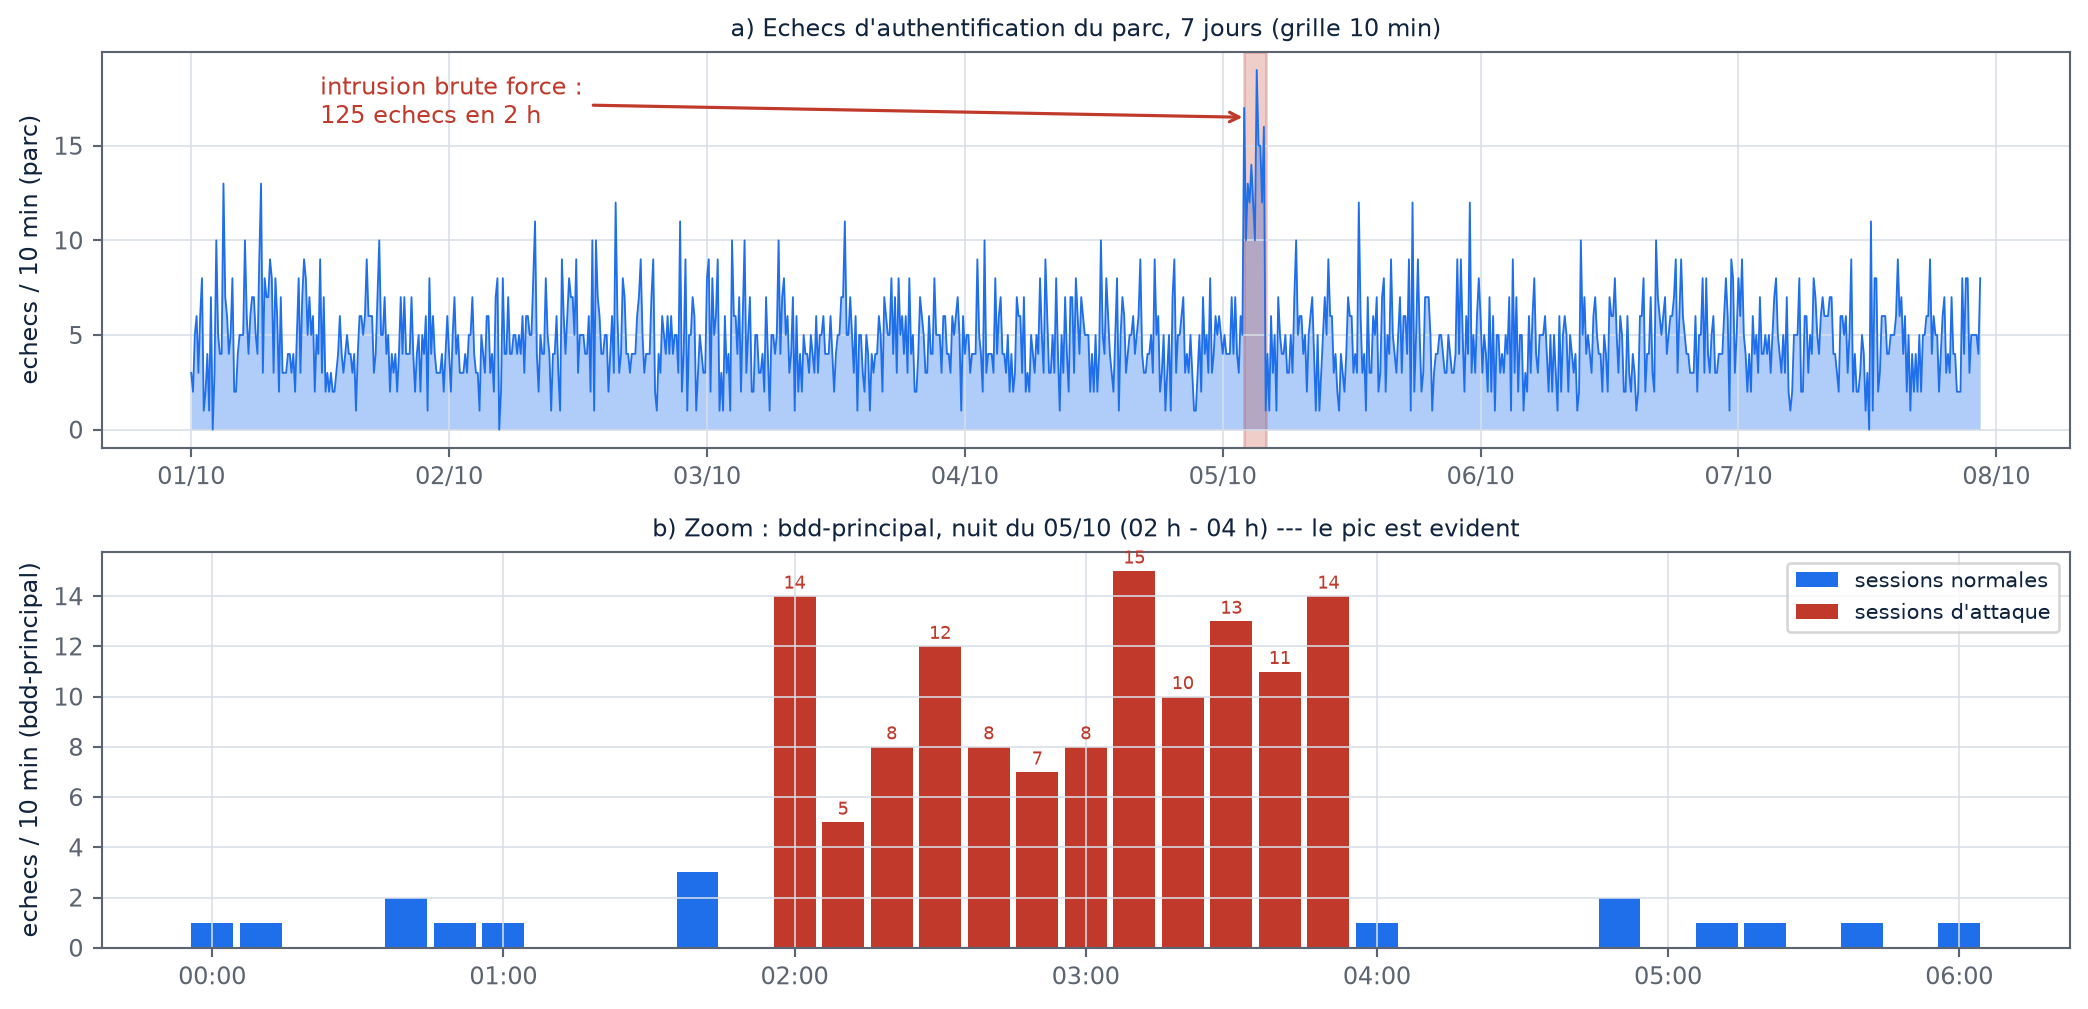
\includegraphics[width=0.90\textwidth]{f29_echecs_7j.png}
\end{center}
\end{column}
\end{columns}
\end{frame}

\begin{frame}{Étape 2 : les features d'attaque par session}
\begin{center}
\footnotesize
\begin{tabular}{@{}p{4.1cm}p{5.4cm}p{2.6cm}@{}}
\toprule
\textbf{Feature} & \textbf{Intuition de détection} & \textbf{Attaque mesurée}\\
\midrule
\py{echecs} & un brute force empile les échecs & moyenne \textbf{10,4}, max 15\\
\py{taux\_echec} & échecs / événements de la session & $= 1{,}0$ (zéro succès)\\
\py{echecs\_consecutifs} & rafale ininterrompue $=$ signature forte & jusqu'à 15\\
\py{utilisateurs} & le robot teste des comptes en série & 3,7 en moyenne\\
\py{entropie} & diversité des comptes testés (bits) & 1,73 vs 2,22 en normal\\
\py{comptes\_sensibles} & échecs sur \py{root}, \py{admin}, \py{inconnu-*} & \textbf{100 \%} des échecs\\
\py{nuit} & fenêtre 22 h -- 06 h & toutes les sessions\\
\bottomrule
\end{tabular}
\end{center}
\vspace{1mm}
\begin{kbox}[Aucune feature ne suffit seule]
Le maximum de la baseline est \textbf{4 échecs / session} --- un seuil sur
\py{echecs} marcherait ici. Mais une session normale de nuit à 3 échecs sur
des comptes variés a une \textbf{entropie haute} (2,2 bits) alors que
l'attaque teste une \emph{petite liste} de comptes (1,73 bit). Combiner
$\ge 2$ features faibles $=$ l'idée centrale du ML de sécurité.
\end{kbox}
\end{frame}

\begin{frame}{L'entropie de Shannon des comptes testés}
\footnotesize%
\begin{columns}[t]
\begin{column}{0.5\textwidth}
\begin{block}{La formule (en bits)}
$H = -\sum_i p_i \log_2 p_i$, où $p_i$ est la part des essais portant sur
le compte $i$.
\begin{itemize}
\item Tous les essais sur \emph{un seul} compte : $H = 0$.
\item Essais uniformément répartis sur $k$ comptes : $H = \log_2 k$.
\item Un brute force humain outillé teste une \textbf{petite liste ordonnée}
(\py{root}, \py{admin}, comptes par défaut) : entropie \emph{basse} à
l'échelle de la session.
\end{itemize}
\end{block}
\begin{ebox}[En pratique avec scipy]
\py{scipy.stats.entropy(comptage, base=2)} --- ou à la main :
\py{-sum(p*log2(p) for p in frequences)}. C'est la tâche B2 du TP.
\end{ebox}
\end{column}
\begin{column}{0.46\textwidth}
\begin{center}
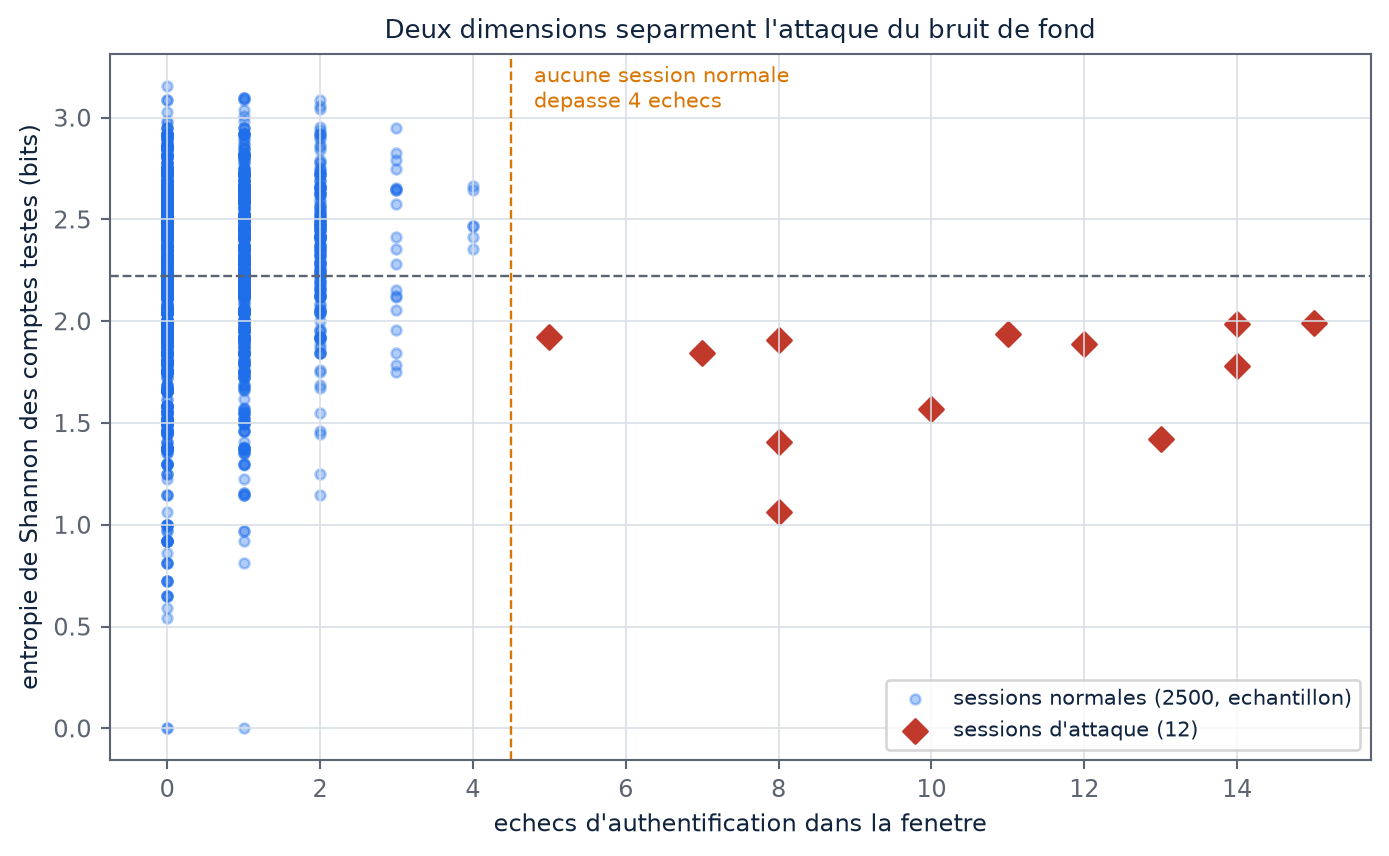
\includegraphics[width=\textwidth]{f30_entropie_echecs.png}
\end{center}
\end{column}
\end{columns}
\end{frame}

\begin{frame}[fragile]{IsolationForest : isoler l'anormal, pas décrire le normal}
\begin{columns}[t]
\begin{column}{0.52\textwidth}
\begin{block}{Le principe en trois phrases}
Une forêt d'arbres coupe l'espace des features au hasard. Une session
\textbf{isolée} (loin des autres, dans une région clairsemée) tombe dans une
feuille après \textbf{peu de coupes} ; une session du flot normal demande
beaucoup de coupes. Le score d'anomalie mesure cette facilité d'isolement.
\end{block}
\begin{itemize}
\item Non supervisé : \textbf{aucune étiquette} d'attaque nécessaire.
\item \py{contamination} : la fraction d'anomalies attendue (ici 0,005)
--- c'est \emph{notre a priori}, pas une vérité mesurée.
\item Alternatives : \py{LocalOutlierFactor} (densité locale),
autoencodeurs (reconstruction).
\end{itemize}
\end{column}
\begin{column}{0.44\textwidth}
\begin{codebox}[Le cœur de B3]
\begin{lstlisting}
iso = IsolationForest(
    n_estimators=200,
    contamination=0.005,
    random_state=5534, n_jobs=2)
iso.fit(X)                    # X = sessions x 7 features
score = -iso.decision_function(X)
top = S.assign(score=score)\
       .sort_values("score",
                    ascending=False)
top30 = top.head(30)          # l'analyste
                              # ne lit que ca
\end{lstlisting}
\end{codebox}
\end{column}
\end{columns}
\vspace{1mm}
\begin{center}\small
Seuil de décision $\ne$ vérité : on juge le détecteur par son
\textbf{classement} (précision@N), pas par une étiquette binaire.
\end{center}
\end{frame}

\begin{frame}{Résultat réel : toutes les sessions d'attaque au top 12}
\footnotesize%
\begin{columns}[t]
\begin{column}{0.5\textwidth}
\begin{center}
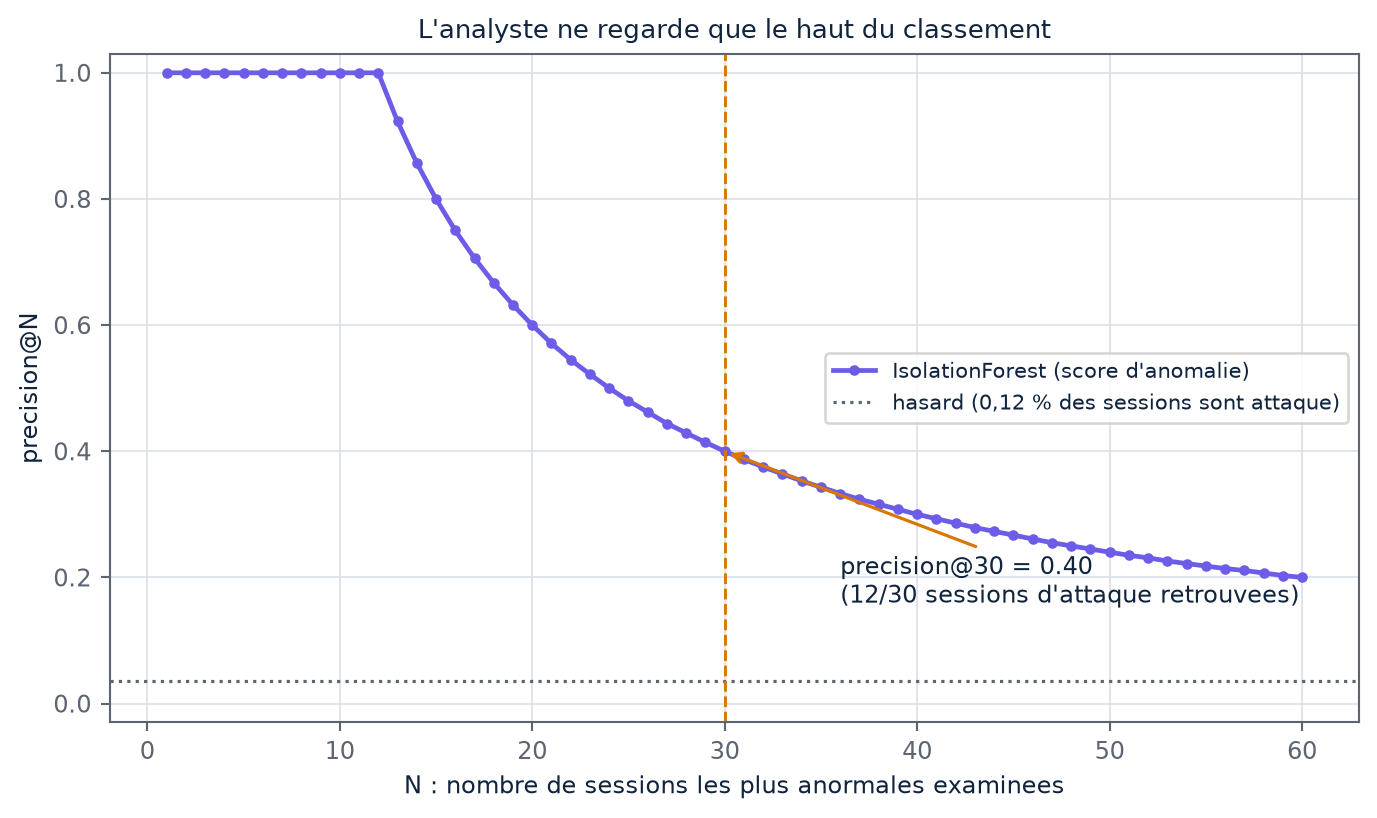
\includegraphics[width=\textwidth]{f31_precision_at_n.png}
\end{center}
\end{column}
\begin{column}{0.46\textwidth}
\begin{ebox}[Chiffres mesurés (graine 5534)]
\begin{itemize}
\item Rangs 1 à 12 : \textbf{exactement les 12 sessions d'attaque}.
\item \textbf{précision@10 $= 1{,}00$}, précision@30 $= 0{,}40$,
précision@50 $= 0{,}24$.
\item Rappel (top 30) $= 1{,}00$ : rien n'est manqué.
\item Par hasard, précision@30 serait $\approx$ 0,0012 :
\textbf{$\times$ 333 mieux que le hasard}.
\end{itemize}
\end{ebox}
\begin{wbox}[Lire la décroissance]
Au-delà du rang 12, précision@N décroît : les sessions « anormales mais
normales » (4 échecs de service, 7 utilisateurs) remontent. \textbf{Le
classement est un curseur} : l'analyste descend jusqu'à ce que le coût de
lecture dépasse la valeur des alertes.
\end{wbox}
\end{column}
\end{columns}
\end{frame}

\begin{frame}{Regrouper les alertes : le clustering rattache l'attaque}
\begin{columns}[t]
\begin{column}{0.5\textwidth}
\begin{block}{Pourquoi regrouper ?}
12 sessions d'attaque $=$ 12 alertes séparées... ou \textbf{1 incident} sur
2 heures. Sans regroupement, l'analyste croit à 12 problèmes distincts ;
avec, il voit \emph{une} campagne coordonnée sur \py{bdd-principal}.
\end{block}
\begin{itemize}
\item \py{DBSCAN} sur (machine encodée, heure, features) : les sessions
d'attaque partagent machine et fenêtres adjacentes $\Rightarrow$ un seul
cluster dense, le bruit reste \py{-1}.
\item Plus simple et robuste : \textbf{fusionner} les sessions anormales de
la même machine séparées de $\le$ 2 fenêtres.
\end{itemize}
\end{column}
\begin{column}{0.46\textwidth}
\begin{kbox}[De session à incident]
La sortie du détecteur n'est pas « 12 alertes » mais :
\begin{center}
\emph{« Campagne de brute force,\\ bdd-principal, 05/10 02 h -- 04 h,\\
125 échecs, comptes root/admin/inconnu-* »}
\end{center}
C'est la granularité que l'exploitant sait traiter --- et la base du
\textbf{livrable B5} du TP.
\end{kbox}
\end{column}
\end{columns}
\end{frame}

\begin{frame}{Quiz 2 --- sessions et détection non supervisée (5 min)}
\begin{qbox}[3 questions]
\begin{enumerate}
\item Pourquoi agréger en sessions de 10 min plutôt qu'analyser ligne par ligne ?\\
(a) c'est plus rapide \quad (b) une ligne ne dit rien : l'anomalie est dans la
\emph{densité} et la \emph{combinaison} d'événements \quad (c) parce que les
logs sont trop gros
\item Une session teste 8 comptes parfaitement équilibrés. Entropie :\\
(a) 0 bit \quad (b) 3 bits \quad (c) 8 bits
\item \py{contamination=0.005} dans IsolationForest signifie :\\
(a) 0,5 \% des données sont infectées \quad (b) un a priori sur la fraction
d'anomalies, qui calibre le seuil de décision \quad (c) le taux de faux positifs
\end{enumerate}
\end{qbox}
\vspace{1mm}
\begin{solbox}[Réponses]
\textbf{1 : b} --- l'agrégation fabrique les features qui portent la signature.
\quad
\textbf{2 : b} --- $\log_2 8 = 3$ bits, distribution uniforme.
\quad
\textbf{3 : b} --- c'est un paramètre d'a priori, à ajuster selon le contexte.
\end{solbox}
\end{frame}

% =====================================================================
%  Seance 5 -- C. supervise : quand on a des etiquettes historiques
% =====================================================================
\section{Quand on a des étiquettes : le détecteur supervisé}

\begin{frame}[fragile]{Le scénario supervisé : les incidents passés sont des étiquettes}
\begin{columns}[t]
\begin{column}{0.5\textwidth}
\begin{block}{Etiqueter les sessions}
Ici, « vérité terrain » : les sessions de la fenêtre d'attaque réelle
(bdd-principal, 02 h -- 04 h le 05/10) $=$ \textbf{1}, les 9\,988 autres
$=$ \textbf{0}. En production, ces étiquettes viennent des tickets
d'incident, des rapports du SOC, des post-mortems.
\end{block}
\begin{itemize}
\item Problème : \textbf{12 positives sur 10\,000} --- déséquilibre extrême
(0,12 \%), comme les 120 fenêtres incident de la séance 2.
\item Réponses : \py{class\_weight="balanced"}, forêt robuste, évaluation
stratifiée.
\item Split : 50 \% train / 50 \% test \textbf{stratifié}, graine 5534 ---
6 positives en test.
\end{itemize}
\end{column}
\begin{column}{0.46\textwidth}
\begin{codebox}[Le cœur de B4]
\begin{lstlisting}
rf = RandomForestClassifier(
    n_estimators=300,
    class_weight="balanced",
    random_state=5534, n_jobs=2)
rf.fit(X_train, y_train)
pred = rf.predict(X_test)
precision_score(y_test, pred)
recall_score(y_test, pred)
\end{lstlisting}
\end{codebox}
\end{column}
\end{columns}
\end{frame}

\begin{frame}{Resultat réel : non-supervisé vs supervisé}
\begin{columns}[t]
\begin{column}{0.5\textwidth}
\begin{center}
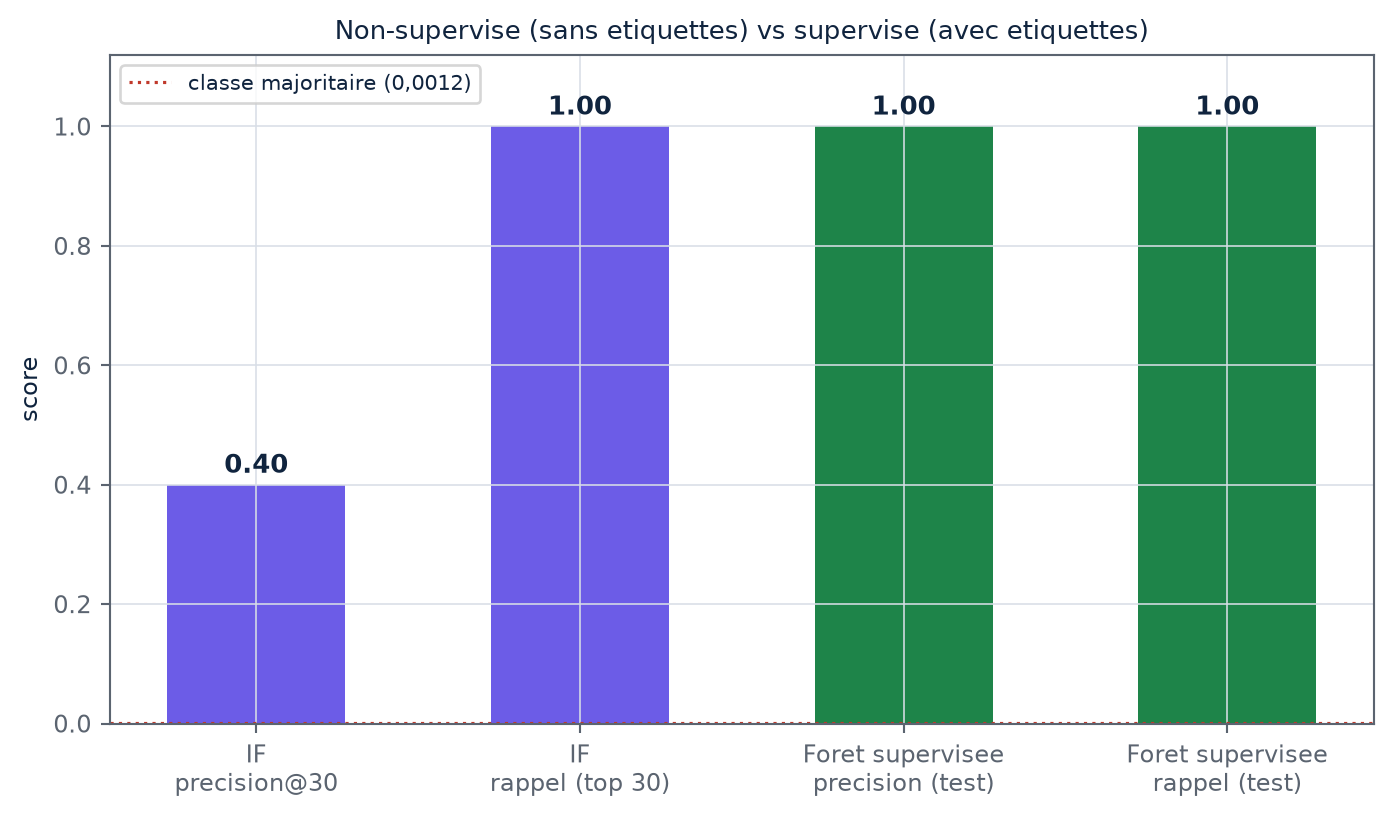
\includegraphics[width=\textwidth]{f32_supervise_vs_non.png}
\end{center}
\end{column}
\begin{column}{0.46\textwidth}
\begin{ebox}[Ce que disent les chiffres]
\begin{itemize}
\item Supervisé : précision \textbf{1,00} et rappel \textbf{1,00} sur le
test (6 positives) --- sur ce jeu, le signal est si net que la forêt sépare
parfaitement.
\item Non supervisé : rappel 1,00 aussi, mais précision@30 $= 0{,}40$ ---
\emph{sans aucune étiquette}.
\end{itemize}
\end{ebox}
\begin{wbox}[Méfiez-vous du 100 \%]
6 positives en test : l'intervalle de confiance est énorme. Un modèle
parfait sur un jeu petit et propre échoue en production (attaque
\emph{différente}, données bruitées). Le 100 \% mesure le jeu, pas la
sécurité du parc.
\end{wbox}
\end{column}
\end{columns}
\end{frame}

\begin{frame}{Ce que la forêt a appris : importance des features}
\begin{center}
\footnotesize
\begin{tabular}{@{}lcc@{}}
\toprule
\textbf{Feature} & \textbf{Importance mesurée} & \textbf{Lecture}\\
\midrule
\py{comptes\_sensibles} & 0,259 & viser \py{root}/\py{admin}/\py{inconnu-*} : signal fort\\
\py{echecs} & 0,226 & le volume d'échecs, attendu\\
\py{echecs\_consecutifs} & 0,219 & la rafale ininterrompue\\
\py{taux\_echec} & 0,213 & zéro succès pendant l'attaque\\
\py{utilisateurs} & 0,051 & contribution secondaire\\
\py{entropie} & 0,030 & redondante avec les échecs ici\\
\py{nuit} & 0,002 & presque inutile sur ce jeu\\
\bottomrule
\end{tabular}
\end{center}
\vspace{1mm}
\begin{kbox}[Les quatre features de tête racontent la même histoire]
Comptes sensibles + échecs + rafale + zéro succès $=$ la \emph{définition}
d'un brute force. La forêt n'a rien inventé : elle a redécouvert la
signature --- et \textbf{quantifié} la contribution de chaque dimension,
ce qu'une règle écrite à la main ne fait pas.
\end{kbox}
\end{frame}

\begin{frame}{Choisir son détecteur : arbre de décision opérationnel}
\footnotesize%
\begin{columns}[t]
\begin{column}{0.52\textwidth}
\begin{block}{Vous n'avez AUCUNE étiquette historique}
$\Rightarrow$ non supervisé (IsolationForest, LOF) + validation par
échantillonnage manuel du top-N. C'est le point d'entrée de \emph{tout}
SOC qui démarre.
\end{block}
\begin{block}{Vous avez des incidents étiquetés, rares}
$\Rightarrow$ supervisé à \py{class\_weight} équilibré ; métriques :
\textbf{rappel d'abord} (rater une intrusion coûte cher), précision ensuite.
\end{block}
\end{column}
\begin{column}{0.44\textwidth}
\begin{block}{Vous avez les deux}
$\Rightarrow$ les deux en production (séance 5 d : redondance des
détecteurs) + le supervisé réentraîné à chaque incident confirmé : la
boucle d'amélioration.
\end{block}
\begin{qbox}[Question]
Vos 10\,000 sessions n'ont \emph{aucune} étiquette fiable. Pourquoi ne pas
étiquetter « session à $>$ 5 échecs $=$ attaque » et entraîner là-dessus ?\\
(a) c'est trop lent \quad (b) c'est circulaire : le modèle apprendrait votre
règle, jamais mieux qu'elle \quad (c) les forêts n'aiment pas les étiquettes
\end{qbox}
\end{column}
\end{columns}
\end{frame}

\begin{frame}{Quiz 3 --- supervisé et évaluation (5 min)}
\begin{qbox}[3 questions]
\begin{enumerate}
\item Avec 12 positives sur 10\,000 sessions, la métrique à surveiller en
priorité est :\\
(a) l'exactitude globale \quad (b) le rappel et la précision sur la classe
rare \quad (c) le score R²
\item Précision@30 $= 0{,}40$ signifie :\\
(a) 40 \% de l'attaque est bloquée \quad (b) parmi les 30 sessions les plus
anormales, 12 sont de vraies attaques \quad (c) le modèle se trompe 40 \% du temps
\item Le meilleur usage des incidents confirmés par les analystes est :\\
(a) les archiver \quad (b) en faire des étiquettes pour réentraîner le
détecteur supervisé \quad (c) baisser le seuil d'alerte
\end{enumerate}
\end{qbox}
\vspace{1mm}
\begin{solbox}[Réponses]
\textbf{1 : b} --- l'exactitude est piégeuse (99,88 \% en prédisant « rien »).
\quad
\textbf{2 : b} --- précision@N juge le \emph{classement}, l'outil de l'analyste.
\quad
\textbf{3 : b} --- c'est la boucle non supervisé $\rightarrow$ supervisé.
\end{solbox}
\end{frame}

% =====================================================================
%  Seance 5 -- D. fiabilite du detecteur + limites (obligatoire)
% =====================================================================
\section{Fiabilité du détecteur et limites}

\begin{frame}{Fiabilité 1 : la dérive de modèle}
\footnotesize%
\begin{columns}[t]
\begin{column}{0.52\textwidth}
\begin{block}{Le trafic change, le modèle vieillit}
\begin{itemize}
\item Lundi : nouveau service batch qui se connecte toutes les nuits à 3 h.
\item Un mois plus tard : rotation des mots de passe, politiques de comptes
modifiées, croissance du parc.
\item Le « normal » appris en octobre n'est plus le normal de décembre :
les scores dérivent, les faux positifs s'accumulent \textbf{sans aucune
erreur visible}.
\end{itemize}
\end{block}
\begin{ebox}[Les garde-fous]
\begin{itemize}
\item Surveiller la \textbf{distribution des features} elles-mêmes
(PSI, KS test) : alarme si le normal bouge.
\item Réentraîner sur fenêtre glissante (30-90 j) --- et garder une
référence figée pour comparer.
\item Chaque incident confirmé $=$ étiquette neuve (boucle du cours 2).
\end{itemize}
\end{ebox}
\end{column}
\begin{column}{0.44\textwidth}
\begin{kbox}[Lien avec les séances précédentes]
C'est la \textbf{même dérive} que le capteur de srv-06 (séance 2), mais sur
les features de sécurité au lieu de la température. La leçon est la même :
\textbf{un modèle non surveillé est un capteur qui ment paisiblement}.
\end{kbox}
\begin{wbox}[Le piège du réentraînement]
Si l'attaquant revient toutes les semaines, le réentraînement glissant
\textbf{apprend l'attaque comme normal}. Fixer la fenêtre, surveiller les
scores, garder l'humain dans la boucle.
\end{wbox}
\end{column}
\end{columns}
\end{frame}

\begin{frame}{Fiabilité 2 : la qualité des données en production}
\footnotesize%
\begin{columns}[t]
\begin{column}{0.5\textwidth}
\begin{block}{Ce qui casse un détecteur de sécurité sans prévenir}
\begin{itemize}
\item \textbf{Horloges} : un serveur en retard déplace ses événements de
fenêtre --- fausse rafale, vrai faux positif.
\item \textbf{Collecte perdue} : agent tombé $=$ fenêtres vides $=$
aveugle pendant l'attaque. Surveiller le \emph{volume} de logs par machine !
\item \textbf{Champ trompeur} : dans nos logs, des lignes « Rotation des
logs » ou « Sauvegarde » portent aussi \py{auth\_reussie = False}.
Compter bêtement les \py{False} donne 4\,828 échecs dont beaucoup ne sont
pas des authentifications : \textbf{filtrer d'abord, compter ensuite}.
\end{itemize}
\end{block}
\end{column}
\begin{column}{0.46\textwidth}
\begin{block}{Les réflexes de la séance 2, rejoués en sécurité}
\begin{itemize}
\item Compte de lignes par machine et par jour (trous de collecte).
\item Validation de schéma (types, niveaux attendus).
\item Vérification croisée : le volume d'échecs d'une machine ne peut pas
être 10$\times$ la médiane sans que \emph{quelque chose} se passe ---
mais est-ce une attaque ou un défaut d'agent ?
\end{itemize}
\end{block}
\begin{kbox}[Règle]
\textbf{Un détecteur est aussi fiable que sa pipeline de données.}
Le ML ne corrige pas un capteur menteur.
\end{kbox}
\end{column}
\end{columns}
\end{frame}

\begin{frame}{Fiabilité 3 : la redondance des détecteurs}
\begin{center}
\footnotesize
\begin{tabular}{@{}p{3.6cm}p{3.4cm}p{3.4cm}@{}}
\toprule
 & \textbf{Règle (seuil 5 échecs/10 min)} & \textbf{Modèle (7 features)}\\
\midrule
Attaque grossière (notre brute force) & \ok{} détecte (12/12) & \ok{} détecte (12/12)\\
\addlinespace[1pt]
Attaque lente (4 échecs/10 min) & \nok{} invisible & \ok{} visible (entropie, comptes, nuit)\\
\addlinespace[1pt]
Bruit opérationnel (défauts de service) & \nok{} faux positifs possibles & \ok{} absorbé par le contexte\\
\addlinespace[1pt]
Explication à donner & \ok{} triviale & $\approx$ SHAP (slide suivante)\\
\addlinespace[1pt]
Coût de maintenance & règle à réviser à chaque changement & réentraînement, surveillance de dérive\\
\bottomrule
\end{tabular}
\end{center}
\vspace{1mm}
\begin{kbox}[Défense en profondeur, version ML]
Règles et modèle fonctionnent \textbf{en parallèle}, jamais l'un à la place
de l'autre : la règle couvre le cas trivial et sert de référence explicite ;
le modèle couvre l'espace que la règle ne sait pas formuler. Une alerte
confirmée par les deux canaux monte en priorité.
\end{kbox}
\end{frame}

\begin{frame}{Limite 1 : l'attaque adversariale}
\begin{columns}[t]
\begin{column}{0.52\textwidth}
\begin{block}{L'attaquant connaît (ou teste) votre détecteur}
S'il sait que le top du classement regarde échecs, rafales et comptes
sensibles, il s'adapte :
\begin{itemize}
\item ralentir : 2 échecs / 10 min, attaque étalée sur 20 h ;
\item doper l'entropie : tester beaucoup de comptes plausibles, même faux ;
\item passer par des comptes ordinaires (\py{dev1}) au lieu de \py{root}.
\end{itemize}
Chaque contremesure dégrade \emph{les mêmes features} que le modèle utilise.
\end{block}
\end{column}
\begin{column}{0.44\textwidth}
\begin{ebox}[Ce que ça coûte à l'attaquant]
Ralentir à 2 échecs/10 min multiplie la durée de l'attaque par 5
(2 h $\rightarrow$ 10 h pour 125 essais) : plus de temps de détection
par d'autres canaux, plus de chances qu'un gardien remarque les connexions
de nuit. \textbf{Le ML ne stoppe pas l'attaquant, il le coûteux.}
\end{ebox}
\begin{kbox}[La parade]
Horloge d'émission, cadence inter-essais, source réseau, corrélations entre
machines. Varier et \textbf{ne pas documenter} toutes les dimensions de détection.
\end{kbox}
\end{column}
\end{columns}
\end{frame}

\begin{frame}{Limite 2 : la fatigue d'alerte --- Limite 3 : l'explicabilité}
\footnotesize%
\begin{columns}[t]
\begin{column}{0.5\textwidth}
\begin{block}{Fatigue d'alerte}
Trop de faux positifs $\Rightarrow$ les analystes \textbf{clichent sans
regarder} $\Rightarrow$ la vraie attaque passe au milieu. C'est ce qui s'est
passé à Target (2013) : les alarmes existaient, personne ne les lisait plus.
\begin{itemize}
\item Mesure : \textbf{taux de traitement} des alertes, précision@N
\emph{en conditions réelles}.
\item Remède : classer (précision@N), regrouper (clustering), seuil haut +
revue périodique du rang 30-100.
\end{itemize}
\end{block}
\end{column}
\begin{column}{0.46\textwidth}
\begin{block}{Explicabilité : SHAP en un aperçu}
SHAP attribue à \textbf{chaque feature sa part} dans la décision d'une
session donnée. Pour notre session n°1 (15 échecs, tous sur comptes
sensibles) : l'attribution pointe d'abord les échecs sur comptes sensibles,
puis la rafale et le taux d'échec --- cohérent avec les importances
mesurées à la slide précédente.
L'analyste reçoit non pas « anormal » mais \emph{pourquoi}. Un modèle
explicable est un modèle qu'on ose couper en incident.
\end{block}
\end{column}
\end{columns}
\vspace{1mm}
\begin{wbox}[Le cercle vicieux à éviter]
Alertes non traitées $\rightarrow$ étiquettes jamais produites $\rightarrow$
détecteur supervisé impossible à améliorer $\rightarrow$ encore plus de faux
positifs. Traiter les alertes, c'est \textbf{alimenter} le système.
\end{wbox}
\end{frame}

\begin{frame}{Limite 4 : la vie privée des logs}
\begin{columns}[t]
\begin{column}{0.5\textwidth}
\begin{block}{Un log d'authentification est une donnée personnelle}
Il dit \emph{qui} était où, quand, sur quelle machine. Nos colonnes :
\py{utilisateur}, \py{machine}, \py{horodatage} --- la combinaison reconstitue
des habitudes de travail (horaires, localisation, usages).
\end{block}
\begin{itemize}
\item \textbf{Pseudonymisation} : remplacer \py{dev1} par un identifiant
op$\;$\#417 (table de correspondance hors zone d'analyse, accès restreint).
\item Les features calculées (échecs, entropie, compte \emph{nombre} de
comptes) survivent à la pseudonymisation : le ML n'a pas besoin des noms.
\item Durée de conservation minimale, accès journalisés, minimisation des
colonnes.
\end{itemize}
\end{column}
\begin{column}{0.46\textwidth}
\begin{ebox}[Notre TP, version conforme]
\begin{itemize}
\item Entraîner le détecteur sur les \textbf{features}, pas sur les noms.
\item Ne révéler les identités que dans la \textbf{note d'incident}, après
corrélation autorisée --- c'est le livrable B5.
\item Les comptes \py{inconnu-1}, \py{inconnu-2} du jeu sont déjà l'exemple
idéal : des pseudos, et l'attaque reste parfaitement détectable.
\end{itemize}
\end{ebox}
\begin{kbox}[Éthique et efficacité vont ensemble]
Un détecteur pseudonymisé est \emph{moins} exposé aux abus internes ---
et fonctionne aussi bien. Penser privacy by design n'est pas une contrainte
de plus : c'est une architecture.
\end{kbox}
\end{column}
\end{columns}
\end{frame}

% =====================================================================
%  Seance 5 -- E. TP B1-B5, quiz de synthese, kbox, preview seance 6
% =====================================================================
\section{TP « Détecter l'intrusion de NOSYS » et synthèse}

\begin{frame}{Le TP : objectif final, une note d'incident}
\begin{columns}[t]
\begin{column}{0.52\textwidth}
\begin{kbox}[Ce que vous produisez à 18 h]
\begin{center}
\file{sessions\_suspectes.csv} + \textbf{note d'incident (1 page)}\\[1mm]
une ligne $=$ (machine, fenêtre 10 min)\\[1mm]
\begin{tabular}{@{}l@{}}
\toprule
echecs, succes, utilisateurs, entropie\\
echecs\_consecutifs, comptes\_sensibles, nuit\\
score\_anomalie (IsolationForest)\\
pred\_attaque (forêt supervisée)\\
\bottomrule
\end{tabular}
\end{center}
\end{kbox}
\begin{ebox}[Chiffres attendus (mesurés)]
\textbf{10\,000 sessions} dont \textbf{12 d'attaque} (0,12 \%) ;
top 30 de l'IF $=$ les 12 sessions d'attaque aux \textbf{rangs 1--12},
précision@30 $= 0{,}40$, rappel $= 1{,}00$ ; forêt supervisée :
précision $=$ rappel $= 1{,}00$ en test stratifié.
\end{ebox}
\end{column}
\begin{column}{0.44\textwidth}
\begin{wbox}[Barème (20 points)]
\begin{itemize}
\item B1 parsing + agrégation : \textbf{4 pts}
\item B2 features + entropie : \textbf{4 pts}
\item B3 IsolationForest + précision@30 : \textbf{5 pts}
\item B4 forêt supervisée + métriques : \textbf{4 pts}
\item B5 livrable + note d'incident : \textbf{3 pts}
\end{itemize}
Graine \textbf{5534} partout, \textbf{2 threads} max. Le code doit
s'exécuter de bout en bout sur \file{nosys\_logs.csv}.
\end{wbox}
\end{column}
\end{columns}
\end{frame}

\begin{frame}[fragile]{TP B1 --- parser et agréger (30 min)}
\begin{codebox}[B1. De 100 000 lignes à 10 000 sessions]
\begin{lstlisting}
import pandas as pd

L = pd.read_csv("data/nosys_logs.csv", parse_dates=["horodatage"])
L["echec"]  = (~L["auth_reussie"].astype(bool)).astype(int)
L["succes"] = 1 - L["echec"]
L["fenetre"] = L["horodatage"].dt.floor("10min")

g = L.groupby(["machine", "fenetre"])
S = pd.DataFrame({
    "n_evenements": g.size(),
    "echecs":  g["echec"].sum(),
    "succes":  g["succes"].sum(),
    "utilisateurs": g["utilisateur"].nunique(),
})
S["taux_echec"] = S["echecs"] / S["n_evenements"]
print(len(S))            # 10000 sessions
print(S["echecs"].max()) # 15  (la rafale de l'attaque)
\end{lstlisting}
\end{codebox}
\vspace{1mm}
\begin{solbox}[Vérification attendue]
10\,000 sessions ; max \py{echecs} $= 15$ (bdd-principal, 03 h 10) ;
moyenne d'échecs par session $\approx 0{,}48$ --- l'attaque dépasse la
normale d'un facteur 20 sur sa feature principale.
\end{solbox}
\end{frame}

\begin{frame}[fragile]{TP B2 --- features d'attaque et entropie (30 min)}
\begin{codebox}[B2. Entropie de Shannon des comptes testés]
\begin{lstlisting}
from scipy.stats import entropy

def entropie_comptes(u):          # u = liste des utilisateurs
    comptage = pd.Series(list(u)).value_counts().values
    return entropy(comptage, base=2)

S["entropie"] = g["utilisateur"].apply(entropie_comptes)

# echecs consecutifs max (la rafale), ordre horaire
def max_run(d):
    e = d.sort_values("horodatage")["echec"].values
    best = cur = 0
    for v in e:
        cur = cur + 1 if v else 0
        best = max(best, cur)
    return best

S["echecs_consecutifs"] = g.apply(max_run, include_groups=False)
SENS = {"root", "admin", "inconnu-1", "inconnu-2"}
S["comptes_sensibles"] = g.apply(
    lambda d: int(d.loc[d["echec"]==1,
                        "utilisateur"].isin(SENS).sum()),
    include_groups=False)
S["nuit"] = (S.index.get_level_values("fenetre").hour < 6)
\end{lstlisting}
\end{codebox}
\vspace{1mm}
\begin{center}\small
Vérification : entropie moyenne attaque $\approx 1{,}73$ bits vs
$2{,}22$ bits sur le reste ; \textbf{100 \%} des échecs d'attaque portent
sur des comptes sensibles.
\end{center}
\end{frame}

\begin{frame}[fragile]{TP B3 --- IsolationForest et précision@30 (30 min)}
\footnotesize%
\begin{codebox}[B3. Classer, puis compter le recouvrement]
\begin{lstlisting}
from sklearn.ensemble import IsolationForest

FEATS = ["echecs", "taux_echec", "utilisateurs", "entropie",
         "echecs_consecutifs", "comptes_sensibles", "nuit"]
X = S[FEATS].values

iso = IsolationForest(n_estimators=200, contamination=0.005,
                      random_state=5534, n_jobs=2)
S["score"] = -iso.fit(X).decision_function(X)
top30 = S.sort_values("score", ascending=False).head(30)

# verite terrain : fenetre d'attaque reelle
att = (top30["machine"] == "bdd-principal") & \
      top30["fenetre"].between("2026-10-05 02:00",
                               "2026-10-05 04:00")
print("precision@30 :", att.mean())   # 0.40
print("rappel :", ...)                 # 12/12 = 1.0
\end{lstlisting}
\end{codebox}
\vspace{1mm}
\begin{center}\small
Attendu : les 12 sessions d'attaque occupent les \textbf{rangs 1 à 12}.
Discutez : pourquoi précision@10 $= 1{,}0$ mais précision@30 $= 0{,}4$ ?
\end{center}
\end{frame}

\begin{frame}[fragile]{TP B4 --- forêt supervisée ; B5 --- livrable (30 min)}
\begin{columns}[t]
\begin{column}{0.52\textwidth}
\begin{codebox}[B4. Supervisé sur l'étiquette session-attaque]
\begin{lstlisting}
from sklearn.ensemble import RandomForestClassifier
from sklearn.model_selection import \
    train_test_split

S["attaque"] = att_reelle(S)   # fenetre 2-4h bdd
Xtr, Xte, ytr, yte = train_test_split(
    S[FEATS], S["attaque"], test_size=0.5,
    stratify=S["attaque"], random_state=5534)
rf = RandomForestClassifier(
    n_estimators=300, class_weight="balanced",
    random_state=5534, n_jobs=2).fit(Xtr, ytr)
print(precision_score(yte, rf.predict(Xte)))  # 1.0
print(recall_score(yte, rf.predict(Xte)))     # 1.0
\end{lstlisting}
\end{codebox}
\end{column}
\begin{column}{0.44\textwidth}
\begin{ebox}[B5. Livrable (10 min)]
\begin{itemize}
\item \file{sessions\_suspectes.csv} : le top 30 avec score et prédiction.
\item \textbf{Note d'incident (1 page)} : ce qui s'est passé (brute force,
bdd-principal, 05/10 02 h -- 04 h), \textbf{preuve chiffrée} (125 échecs,
12 sessions, comptes ciblés, 0 succès), \textbf{action recommandée}
(ex. blocage IP + verrouillage progressif + rotation des mots de passe).
\end{itemize}
\end{ebox}
\begin{wbox}[Attention]
\py{att\_reelle} ne doit servir \textbf{qu'à l'évaluation} --- l'utiliser
comme feature serait une fuite de données (règle anti-fuite de la séance 2).
\end{wbox}
\end{column}
\end{columns}
\end{frame}

\begin{frame}{Quiz de synthèse --- 5 QCM (10 min)}
\begin{qbox}[Séance 5, tout le programme]
\begin{enumerate}
\item Le premier réflexe face à 100\,000 lignes de logs est de :\\
(a) tout lire \quad (b) agréger en sessions et construire des features \quad
(c) acheter un SIEM
\item La granularité « session » utilisée aujourd'hui est :\\
(a) (utilisateur, jour) \quad (b) (machine, fenêtre 10 min) \quad (c) (message, niveau)
\item IsolationForest a placé les 12 sessions d'attaque :\\
(a) aux rangs 1--12 \quad (b) aux rangs 100--112 \quad (c) nulle part
\item Le superviseur bat le non-supervisé surtout parce qu'il :\\
(a) va plus vite \quad (b) connaît la frontière attaque/normal apprise des
incidents passés \quad (c) n'a pas d'hyperparamètres
\item La meilleure défense contre la fatigue d'alerte est :\\
(a) plus d'alertes \quad (b) classer et regrouper pour ne montrer que le
haut du classement \quad (c) supprimer les règles
\end{enumerate}
\end{qbox}
\vspace{1mm}
\begin{solbox}[Corrigé]
\textbf{1 : b} \quad \textbf{2 : b} \quad \textbf{3 : a} (mesuré, graine 5534) \quad
\textbf{4 : b} \quad \textbf{5 : b}
\end{solbox}
\end{frame}

\begin{frame}{Ce qu'il faut retenir --- et la suite}
\begin{columns}[t]
\begin{column}{0.52\textwidth}
\begin{kbox}[Les 5 idées de la séance]
\begin{enumerate}
\item La signature d'une attaque vit dans l'\textbf{agrégation}, pas dans
la ligne : sessions (machine $\times$ 10 min) et features d'attaque.
\item \textbf{Combiner des signaux faibles} : échecs + entropie + comptes
sensibles + nuit.
\item IsolationForest \textbf{sans étiquette} a retrouvé les 12 sessions
d'attaque aux rangs 1--12 (précision@30 $= 0{,}40$, hasard : 0,0012).
\item Le supervisé (forêt, étiquettes d'incidents) : précision $=$ rappel
$= 1{,}00$ en test --- mais méfiance devant le 100 \%.
\item Limites à garder en tête : adversarial, fatigue d'alerte,
explicabilité (SHAP), vie privée ; fiabilité : dérive, données, redondance.
\end{enumerate}
\end{kbox}
\end{column}
\begin{column}{0.44\textwidth}
\begin{ebox}[Prochaine séance --- Séance 6]
\textbf{MLOps : faire vivre les modèles}
\begin{itemize}
\item Exposer un détecteur en \textbf{API} (endpoint de scoring).
\item \textbf{Réentraînement} automatique : déclencheurs, fenêtres,
validation avant mise en production.
\item Surveillance de bout en bout : données, dérive, scores --- le
pipeline complet de NOSYS, de la collecte à l'alerte.
\end{itemize}
À préparer : relire la séance 3 (forêt, validation croisée) --- la séance 6
met le \emph{modèle} en production, pas seulement le code.
\end{ebox}
\end{column}
\end{columns}
\end{frame}

% =====================================================================
%  Seance 6 -- A. Cours 1 : MLOps pour l'infrastructure (frames 1--10)
% =====================================================================
\section{Séance 6 --- Perspectives et évolutions}
\chapterslide{Séance 6}{Industrialisation et clôture --- MLOps, perspectives, évaluation}
{4 h --- 2 h cours / 2 h TP --- Partie 6 du syllabus EPD-GIT-5534}
{\textbf{Objectifs :} décrire le pipeline MLOps complet (données $\rightarrow$
entraînement $\rightarrow$ validation $\rightarrow$ déploiement $\rightarrow$
monitoring) $\bullet$ décider un plan de \textbf{retraining} et mesurer la
dérive sur les données NOSYS $\bullet$ mesurer la \textbf{latence de scoring}
réelle et raisonner la capacité $\bullet$ connaître les enjeux de
\textbf{gouvernance} (responsabilité, model card, vie privée, auditabilité)
$\bullet$ clôturer la mission NOSYS et préparer l'évaluation de l'UE.}

\begin{frame}{Plan de la séance (4 h)}
\footnotesize%
\begin{columns}[t]
\begin{column}{0.48\textwidth}
\begin{kbox}[Cours magistral --- 2 h]
\begin{enumerate}
\item \textbf{MLOps pour l'infrastructure} (50 min) : le pipeline complet,
retraining, registre de modèles, conteneurisation, monitoring.
\item \textbf{Perspectives} (40 min) : autoencodeurs, LLM au NOC, jumeaux
numériques, edge ML.
\item \textbf{Gouvernance et clôture} (30 min) : responsabilité, model card,
vie privée, synthèse de la mission NOSYS.
\end{enumerate}
\end{kbox}
\end{column}
\begin{column}{0.48\textwidth}
\begin{ebox}[Travaux pratiques --- 2 h]
\small\textbf{« De la forêt au service »} sur \file{nosys\_features.csv} :
\begin{enumerate}
\item B1 --- pipeline joblib + script de scoring (30 min)
\item B2 --- latence de scoring, capacité (30 min)
\item B3 --- fiche MLOps d'une page (30 min)
\item B4 --- quiz blanc de 20 questions (30 min)
\end{enumerate}
\end{ebox}
\end{column}
\end{columns}
\vspace{1mm}
\begin{center}\small
Dernière séance de l'UE : on \textbf{industrialise} ce que les séances 1 à 5
ont construit, puis on regarde ce qui vient après.
\end{center}
\end{frame}

\begin{frame}{Le pipeline MLOps complet}
\begin{center}
\resizebox{0.96\textwidth}{!}{%
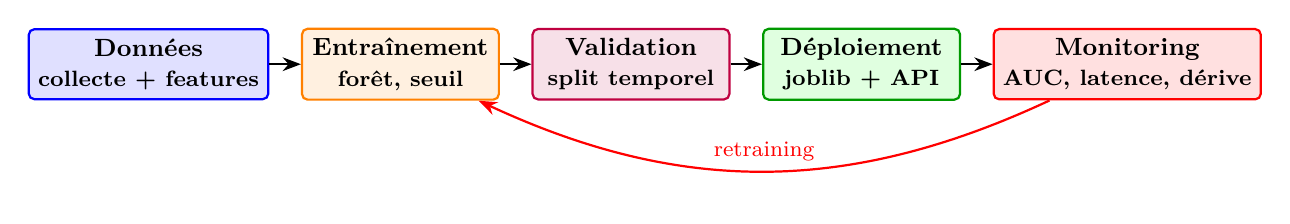
\begin{tikzpicture}[node distance=4mm,
  et/.style={rounded corners=2pt, thick,
             minimum width=2.5cm, minimum height=8mm, align=center,
             font=\small\bfseries}]
\node[et, draw=blue, fill=blue!12]   (d) {Données\\ \footnotesize collecte + features};
\node[et, draw=orange, fill=orange!12, right=of d] (e) {Entraînement\\ \footnotesize forêt, seuil};
\node[et, draw=purple, fill=purple!12, right=of e] (v) {Validation\\ \footnotesize split temporel};
\node[et, draw=green!60!black, fill=green!12, right=of v] (dep) {Déploiement\\ \footnotesize joblib + API};
\node[et, draw=red, fill=red!12, right=of dep] (m) {Monitoring\\ \footnotesize AUC, latence, dérive};
\draw[-{Stealth}, thick] (d) -- (e);
\draw[-{Stealth}, thick] (e) -- (v);
\draw[-{Stealth}, thick] (v) -- (dep);
\draw[-{Stealth}, thick] (dep) -- (m);
\draw[-{Stealth}, thick, red] (m) to[bend left=25] node[above, font=\footnotesize, text=red]{retraining} (e);
\end{tikzpicture}}
\end{center}
\vspace{2mm}
\begin{kbox}[La différence entre un notebook et un système]
Les séances 1 à 5 ont construit la \textbf{chaîne centrale} (données
$\to$ entraînement $\to$ validation). Un modèle qui aide
vraiment l'exploitation vit dans un \textbf{cycle fermé} : la production
reproduit de nouvelles données, le monitoring détecte la dérive, le
retraining referme la boucle. Aujourd'hui on construit le maillon manquant.
\end{kbox}
\end{frame}

\begin{frame}{Du notebook au service : ce qui change}
\small
\begin{columns}[t]
\begin{column}{0.5\textwidth}
\begin{block}{Dans le notebook (séances 3--5)}
\begin{itemize}
\item Le modèle vit dans une variable Python, en mémoire.
\item Le split train/test est écrit à la main.
\item Les prédictions sont faites par la même personne qui entraîne.
\end{itemize}
\end{block}
\begin{block}{En production}
\begin{itemize}
\item Le modèle est un \textbf{fichier versionné}, chargé par un service.
\item Le split est \textbf{temporel et automatique} (reproductible).
\item Le scoring tourne \textbf{seul}, 24 h/24, sans humain.
\end{itemize}
\end{block}
\end{column}
\begin{column}{0.46\textwidth}
\begin{wbox}[Le fossé qui fait échouer les projets]
80 \% des projets ML d'infrastructure n'atteignent jamais la production ---
pas à cause du modèle, mais à cause de ce qui l'entoure : versionnement,
tests, monitoring, procédure de \textbf{retour arrière}. C'est le métier du
\textbf{MLOps}.
\end{wbox}
\begin{ebox}[Chiffres réels du dossier NOSYS]
Modèle : forêt de 200 arbres entraînée en \textbf{1,8 s} sur les 24 192
fenêtres du train. Sauvegardée : \textbf{1,1 Mo} en joblib. AUC test :
\textbf{0,80}. C'est petit, c'est tout le pipeline.
\end{ebox}
\end{column}
\end{columns}
\end{frame}

\begin{frame}{Le retraining : quand ré-entraîner ?}
\small
\begin{center}
\begin{tabular}{@{}p{3.2cm}p{4.4cm}p{4.0cm}@{}}
\toprule
\textbf{Déclencheur} & \textbf{Signal observé} & \textbf{Exemple NOSYS}\\
\midrule
\textbf{Dérive mesurée} & AUC qui baisse, scores qui dérivent & proba
moyenne : 0,0001 $\to$ 0,0112 en 8 jours\\
\addlinespace[1pt]
\textbf{Calendrier} & ré-entraînement périodique planifié & dimanche nuit,
charge minimale\\
\addlinespace[1pt]
\textbf{Incident majeur} & un événement change le régime & migration,
nouveau serveur\\
\bottomrule
\end{tabular}
\end{center}
\vspace{1mm}
\begin{wbox}[Le piège du retraining permanent]
Ré-entraîner à chaque alerte détruit l'historique de comparaison : on ne
sait plus \textbf{quelle version} a produit quel comportement. Règle :
ré-entraîner sur déclencheur \textbf{documenté}, valider la nouvelle version
\textbf{contre l'ancienne} sur les mêmes données, puis basculer.
\end{wbox}
\end{frame}

\begin{frame}{La dérive, mesurée sur NOSYS}
\begin{center}
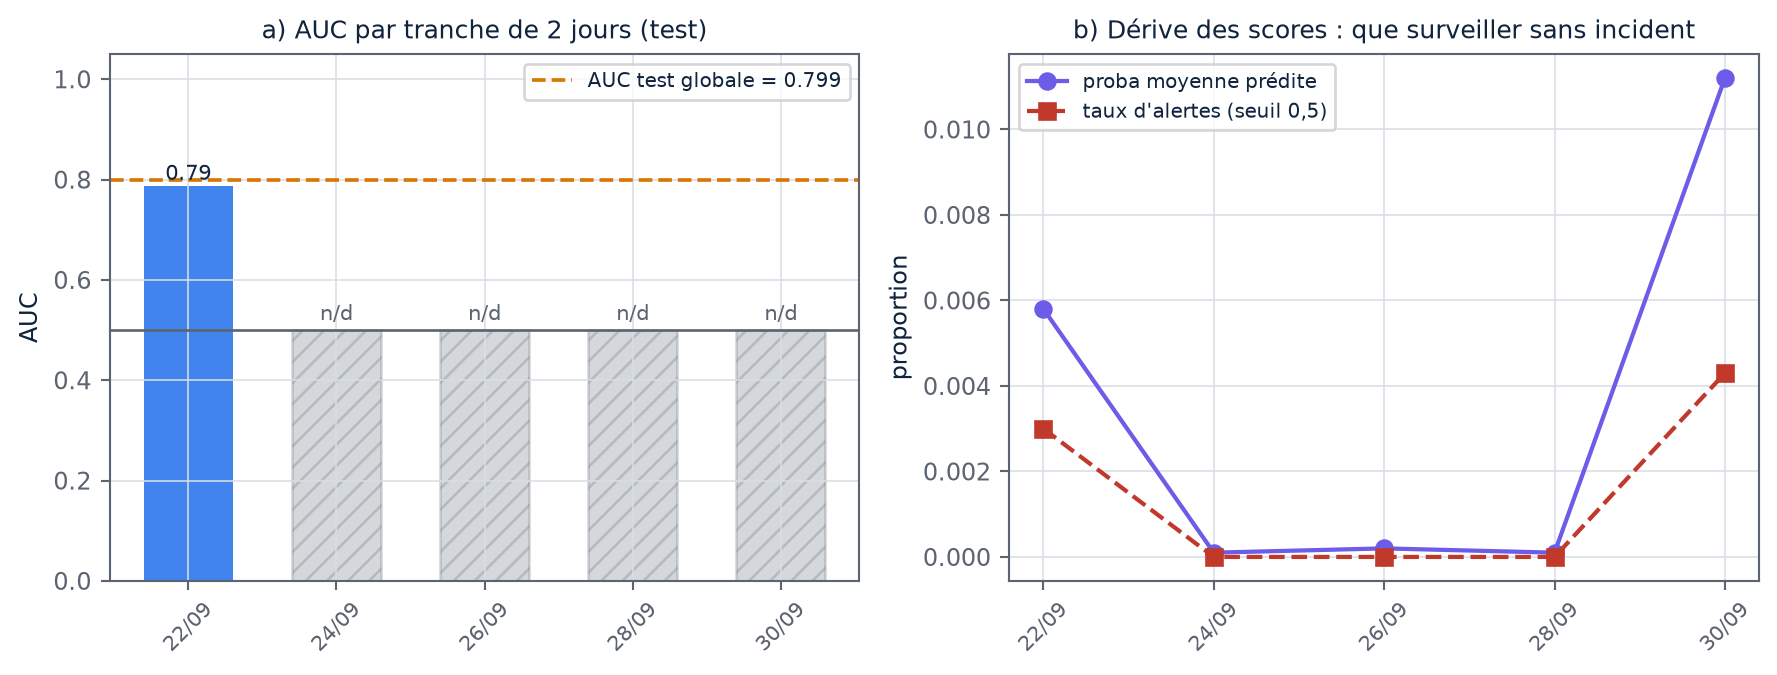
\includegraphics[width=0.80\textwidth]{f33_auc_tranches.png}
\end{center}
\begin{kbox}[Ce que la figure montre (pipeline réel, graine 5534)]
\textbf{a)} L'AUC ne se calcule que sur la tranche du 22/09 (l'incident du
test est concentré là) : \textbf{0,79}, contre \textbf{0,80} sur le test
complet. \textbf{b)} Sans incident, on surveille la \textbf{distribution des
scores} : la proba moyenne remonte de 0,0001 à \textbf{0,0112} et le taux
d'alertes passe à \textbf{0,43 \%} sur la dernière tranche --- signal de
dérive à investiguer avant qu'un incident n'arrive.
\end{kbox}
\end{frame}

\begin{frame}{Le registre de modèles}
\begin{columns}[t]
\begin{column}{0.5\textwidth}
\begin{block}{Ce qu'un registre stocke pour chaque version}
\begin{itemize}
\item Le \textbf{fichier du modèle} (notre \file{.joblib}, 1,1 Mo) et son
empreinte (hash).
\item Les \textbf{données d'entraînement} : fenêtres, colonnes, graine
(\textbf{5534} ici).
\item Les \textbf{métriques de validation} : AUC test 0,80, latence, seuil.
\item Le \textbf{statut} : expérimental, validé, en production, archivé.
\end{itemize}
\end{block}
\end{column}
\begin{column}{0.46\textwidth}
\begin{ebox}[Outils réels]
MLflow, DVC, ou --- suffisant à notre échelle --- un répertoire Git avec un
fichier \file{manifeste.yaml} par version. Le registre répond à une seule
question : \textbf{« quel modèle exactement tournait le 5/10 à 3 h ? »}
\end{ebox}
\begin{wbox}[Lien avec la séance 5]
Le jour de l'intrusion, le registre permet de rejouer les prédictions de la
version en service et de prouver ce que le modèle \textbf{voyait} à ce
moment-là. Sans registre : impossible.
\end{wbox}
\end{column}
\end{columns}
\end{frame}

\begin{frame}[fragile]{Conteneuriser le modèle : Docker en 10 lignes de concept}
\small
\begin{codebox}[L'image = modèle + code de scoring + dépendances figées]
\begin{lstlisting}
FROM python:3.11-slim                    # base figee
WORKDIR /app
COPY nosys_forest.joblib .               # le modele (1,1 Mo)
COPY scorer.py .                         # code de scoring
RUN pip install --no-cache-dir pandas scikit-learn joblib
CMD ["python", "scorer.py"]              # le service
\end{lstlisting}
\end{codebox}
\begin{columns}[t]
\begin{column}{0.48\textwidth}
\begin{kbox}[Pourquoi conteneuriser]
La même image tourne partout : \textbf{mêmes versions} de pandas et
scikit-learn, donc \textbf{mêmes prédictions}. Un modèle qui change de
comportement après une mise à jour de bibliothèque est un incident en
puissance.
\end{kbox}
\end{column}
\begin{column}{0.48\textwidth}
\begin{wbox}[Piège classique]
L'image contient le modèle \textbf{figé au build}. Une nouvelle version du
modèle = une nouvelle image, versionnée et testée --- jamais un écrasement
du fichier en place. C'est le rollback du B3.
\end{wbox}
\end{column}
\end{columns}
\end{frame}

\begin{frame}{Monitoring : que surveiller en production ?}
\begin{center}\footnotesize
\begin{tabular}{@{}p{3.6cm}p{4.4cm}p{4.2cm}@{}}
\toprule
\textbf{Famille} & \textbf{Métrique} & \textbf{Alarme typique}\\
\midrule
Qualité du modèle & AUC recalculée quand la vérité terrain arrive &
AUC $<$ 0,70 pendant 48 h\\
\addlinespace[1pt]
Comportement & taux d'alertes par jour, précision des alertes &
$>$ 3 $\times$ la médiane des 30 derniers jours\\
\addlinespace[1pt]
Santé du service & latence de scoring (moyenne + p99) & p99 $>$ 2 $\times$
la moyenne\\
\addlinespace[1pt]
Entrées & distribution des variables (moyenne, quantiles) & dérive de
\py{cpu\_moy} hors bornes historiques\\
\bottomrule
\end{tabular}
\end{center}
\vspace{1mm}
\begin{kbox}[La règle des deux horloges]
Le monitoring du \textbf{modèle} (AUC, dérive) tourne à l'échelle des
jours ; le monitoring du \textbf{service} (latence, erreurs) tourne à
l'échelle des minutes. Confondre les deux, c'est découvrir un service tombé
une semaine plus tard --- ou alarmer un ingénieur pour une variation de 0,001
d'AUC.
\end{kbox}
\end{frame}

\begin{frame}{Quiz 1 --- MLOps (5 min)}
\begin{qbox}[3 questions]
\begin{enumerate}
\item Le retraining « sur incident majeur » se déclenche quand :\\
(a) une alerte est émise \quad (b) un événement change le régime du système
(migration, nouveau serveur) \quad (c) l'AUC baisse de 0,001
\item Sur les tranches de test sans incident, l'AUC :\\
(a) vaut 0 \quad (b) n'est pas calculable --- on surveille la distribution
des scores \quad (c) vaut 1
\item La version du modèle en production le jour d'un incident se retrouve
grâce à :\\
(a) la mémoire de l'équipe \quad (b) le registre de modèles \quad (c) la
date du fichier
\end{enumerate}
\end{qbox}
\vspace{1mm}
\begin{solbox}[Réponses]
\textbf{1 : b} \quad \textbf{2 : b} --- sans positif, pas d'AUC ; d'où le
suivi de la distribution des scores \quad \textbf{3 : b}
\end{solbox}
\end{frame}

% =====================================================================
%  Seance 6 -- B. Cours 2 : perspectives (frames 11--17)
% =====================================================================
\section{Perspectives : ce qui vient après}

\begin{frame}{Perspectives 1 --- autoencodeurs pour métriques multivariées}
\small
\begin{columns}[t]
\begin{column}{0.52\textwidth}
\begin{block}{Le principe}
Un autoencodeur est un réseau de neurones entraîné à \textbf{reproduire ses
entrées} après un passage par un état compressé. Sur des données normales,
il reconstruit bien. Sur une anomalie, la reconstruction échoue : l'erreur
de reconstruction \textbf{est} le score d'anomalie.
\begin{itemize}
\item Avantage : capte les corrélations \textbf{entre} variables (CPU haut
+ latence normale $=$ suspect même si chaque variable est plausible).
\item Nos 14 variables de \file{nosys\_features.csv} deviennent un vecteur
d'entrée unique.
\end{itemize}
\end{block}
\end{column}
\begin{column}{0.44\textwidth}
\begin{wbox}[Pourquoi pas aujourd'hui]
Sur NOSYS, la forêt atteint déjà \textbf{AUC 0,80} avec 14 variables et
s'explique par importances. Un autoencodeur exige des milliers de fenêtres
normales, se règle difficilement, et son score \textbf{ne s'explique pas}.
Règle d'ingénieur : la complexité se gagne, elle ne s'emprunte pas.
\end{wbox}
\begin{ebox}[Quand il devient pertinent]
Quand le nombre de variables explose (centaines de métriques par service)
et que personne ne peut écrire les features à la main.
\end{ebox}
\end{column}
\end{columns}
\end{frame}

\begin{frame}{Perspectives 2 --- les LLM au NOC (culture, pas TP)}
\begin{center}\small
\begin{tabular}{@{}p{4.2cm}p{8.0cm}@{}}
\toprule
\textbf{Usage} & \textbf{Ce que ça change}\\
\midrule
Résumer un incident & à partir des logs de la nuit du 5/10 (brute force sur
\file{bdd-principal}, $\approx$ 125 échecs), produire en 10 secondes une
note : serveurs touchés, chronologie, actions posées\\
\addlinespace[1pt]
Requête en langage naturel & « donne-moi le p99 de latence de srv-01 la
semaine dernière » traduit en requête de métriques --- l'ingénieur ne
connaît plus la syntaxe par cœur\\
\addlinespace[1pt]
Rédaction de runbooks & transformer un historique de tickets en procédure
réutilisable\\
\bottomrule
\end{tabular}
\end{center}
\vspace{1mm}
\begin{wbox}[Les deux garde-fous à retenir]
\textbf{1.} Un LLM peut \textbf{se tromper avec assurance} : ses sorties sur
un incident se vérifient toujours contre les données brutes. \textbf{2.} On
n'envoie pas des logs contenant des noms d'utilisateurs ou d'adresses IP à
un service externe sans les pseudonymiser (on y revient en gouvernance).
\end{wbox}
\end{frame}

\begin{frame}{Perspectives 3 --- jumeaux numériques}
\small
\begin{columns}[t]
\begin{column}{0.52\textwidth}
\begin{block}{Le principe}
Un \textbf{jumeau numérique} est une simulation du système d'information
assez fidèle pour qu'on y teste des scénarios sans toucher la production :
\begin{itemize}
\item rejouer l'incident du 22/09 et vérifier que le modèle l'aurait
détecté \textbf{plus tôt} ;
\item tester un nouveau seuil ou un nouveau modèle sur \textbf{des mois
d'incidents simulés} en quelques minutes ;
\item entraîner l'équipe du NOC sur des pannes qui n'ont jamais eu lieu.
\end{itemize}
\end{block}
\end{column}
\begin{column}{0.44\textwidth}
\begin{ebox}[Le lien avec nos données]
Nos 30 jours de métriques NOSYS (graine 5534) sont déjà une
\textbf{réplique simplifiée} : un générateur de charge + un injecteur de
défauts. Un jumeau, c'est la même idée avec la topologie réseau en plus.
\end{ebox}
\begin{wbox}[La limite honnête]
Un jumeau reproduit les pannes \textbf{qu'on sait décrire}. La panne
véritablement nouvelle (le cygne noir) n'existe que dans la production ---
d'où le monitoring de la séance précédente, qui reste irremplaçable.
\end{wbox}
\end{column}
\end{columns}
\end{frame}

\begin{frame}{Perspectives 4 --- edge ML : détecter sur l'équipement}
\small
\begin{columns}[t]
\begin{column}{0.52\textwidth}
\begin{block}{Le déplacement du calcul}
Aujourd'hui : les agents envoient les métriques à un serveur central qui
score (notre pipeline). En \textbf{edge ML}, le modèle tourne
\textbf{sur l'équipement} lui-même --- routeur, serveur, passerelle IoT.
\begin{itemize}
\item Détection locale en millisecondes, même si le réseau est coupé
(exactement le scénario d'une vraie panne).
\item Moins de données qui circulent : les métriques brutes restent locales,
seules les alertes partent.
\end{itemize}
\end{block}
\end{column}
\begin{column}{0.44\textwidth}
\begin{wbox}[Le contrainte : la latence, encore]
Sur un équipement, pas de 200 arbres à 60 ms : il faut des modèles
\textbf{compilés et quantifiés} (par ex. arbre unique, modèle linéaire,
micro-réseaux). Le TP B2 prend son sens : mesurer la latence AVANT de
décider où le modèle peut vivre.
\end{wbox}
\begin{kbox}[Fil conducteur]
Toutes ces perspectives (autoencodeurs, edge, jumeaux) changent le
\textbf{modèle ou son lieu d'exécution} --- jamais les fondations :
données propres, split temporel, validation, monitoring.
\end{kbox}
\end{column}
\end{columns}
\end{frame}

\begin{frame}{Quiz 2 --- perspectives (5 min)}
\begin{qbox}[3 questions]
\begin{enumerate}
\item Le score d'anomalie d'un autoencodeur est :\\
(a) la sortie du réseau \quad (b) l'erreur de reconstruction \quad (c) la
distance entre deux points
\item Pourquoi un autoencodeur est-il difficile à justifier devant un
exploitant ?\\
(a) il est trop rapide \quad (b) son score ne s'explique pas par des
variables nommées \quad (c) il exige des étiquettes
\item Le principal intérêt du edge ML pour la détection de panne :\\
(a) plus de précision \quad (b) détecter même si le lien réseau est coupé
\quad (c) un modèle plus gros
\end{enumerate}
\end{qbox}
\vspace{1mm}
\begin{solbox}[Réponses]
\textbf{1 : b} \quad \textbf{2 : b} --- l'interprétabilité reste un critère
de production \quad \textbf{3 : b}
\end{solbox}
\end{frame}

% =====================================================================
%  Seance 6 -- C. Cours 3 : gouvernance + synthese de la mission (18--22)
% =====================================================================
\section{Gouvernance et clôture de la mission NOSYS}

\begin{frame}{Gouvernance 1 --- la responsabilité d'une alerte}
\small
\begin{columns}[t]
\begin{column}{0.5\textwidth}
\footnotesize\begin{block}{Deux scénarios qui arrivent tous les mois}
\begin{itemize}
\item \textbf{Alerte fausse traitée comme vraie} : 3 h perdues. Coût : fatigue, perte de confiance --- la « fatigue d'alertes ».
\item \textbf{Alerte vraie négligée} : l'incident du 22/09 se produit sans
intervention. Coût : indisponibilité, SLA violé.
\end{itemize}
\end{block}
\begin{wbox}[Le principe à retenir]
Le modèle \textbf{propose}, l'humain \textbf{dispose}. La responsabilité
d'une action (couper un service, appeler l'astreinte) reste
\textbf{humaine} --- et le seuil choisi (séance 3) est une décision
d'organisation, pas un réglage technique neutre.
\end{wbox}
\end{column}
\begin{column}{0.46\textwidth}
\begin{ebox}[Ce qu'une bonne organisation documente]
\begin{itemize}
\item Qui a fixé le seuil, quand, sur quelles métriques de validation.
\item Que faire d'une alerte : procédure écrite (runbook), délai cible.
\item Le suivi des faux positifs : chaque alerte fausse est
\textbf{étiquetée} et nourrit le prochain retraining.
\end{itemize}
\end{ebox}
\end{column}
\end{columns}
\end{frame}

\begin{frame}{Gouvernance 2 --- la model card : le modèle a une notice}
\begin{center}\footnotesize
\begin{tabular}{@{}p{3.2cm}p{9.2cm}@{}}
\toprule
\textbf{Rubrique} & \textbf{Contenu pour le modèle NOSYS}\\
\midrule
Objet & prédire une incident sur les 30 min suivantes, par fenêtre de 10 min
et par serveur\\
\addlinespace[1pt]
Données & \file{nosys\_features.csv}, 34 560 fenêtres, 8 serveurs, 30 jours
(split temporel au 22/09)\\
\addlinespace[1pt]
Performances & AUC test \textbf{0,80} ; AUC train 1,00 --- signe de marge de
manoeuvre à surveiller\\
\addlinespace[1pt]
Limites & incidents rares (0,35 \%) ; calibré sur un seul mois ; les
fenêtres sans incident ne permettent pas de mesurer l'AUC\\
\addlinespace[1pt]
Usage prévu & appuyer la décision du NOC --- jamais remplacer la décision
humaine\\
\bottomrule
\end{tabular}
\end{center}
\vspace{1mm}
\begin{kbox}[Une page, versionnée, à côté du modèle]
La model card (Mitchell et al., 2019) est le complément obligatoire du
fichier \file{.joblib} dans le registre. Si vous ne pouvez pas remplir la
rubrique « limites », vous ne connaissez pas assez votre modèle pour le
déployer.
\end{kbox}
\end{frame}

\begin{frame}{Gouvernance 3 --- vie privée des logs et auditabilité}
\footnotesize%
\begin{columns}[t]
\begin{column}{0.5\textwidth}
\begin{block}{Les logs parlent des personnes}
Les logs d'authentification contiennent des identifiants, des adresses IP,
des postes. Avant tout partage (LLM externe, prestataire, archive longue) :
\begin{itemize}
\item \textbf{pseudonymisation} : remplacer l'identifiant par une référence
réversible gardée à part ;
\item \textbf{minimisation} : ne garder que les champs utiles à l'analyse
(l'heure et le résultat d'une tentative, pas le contenu de la session) ;
\item durée de conservation définie et appliquée.
\end{itemize}
\end{block}
\end{column}
\begin{column}{0.46\textwidth}
\begin{block}{Auditabilité}
Pouvoir \textbf{remonter} : quelle version du modèle, sur quelles données,
a produit telle alerte à telle heure. Nos trois clés :
\begin{itemize}
\item registre de modèles (version + hash),
\item graine fixée (\textbf{5534}) $\Rightarrow$ données régénérables,
\item journal des prédictions conservé.
\end{itemize}
\end{block}
\end{column}
\end{columns}
\end{frame}

\begin{frame}{Synthèse de la mission NOSYS --- les 6 livrables de l'UE}
\begin{center}\footnotesize
\begin{tabular}{@{}p{0.7cm}p{4.0cm}p{4.4cm}p{3.2cm}@{}}
\toprule
\textbf{\#} & \textbf{Livrable} & \textbf{Résultat clé} & \textbf{Statut}\\
\midrule
1 & profil et saisonnalité des serveurs & cycle jour/nuit, incident du 09/09 & prêts\\
\addlinespace[1pt]
2 & \file{nosys\_features.csv} supervisé & 34 560 fenêtres, 120 positives
(0,35 \%), 0 fuite & prêts\\
\addlinespace[1pt]
3 & anomalies + classification & forêt : AUC test \textbf{0,80}, seuil calibré & prêts\\
\addlinespace[1pt]
4 & SARIMA + prédiction de panne & rappel 99,94 \% si 70 \% des incidents
évités & prêts\\
\addlinespace[1pt]
5 & analyse des logs, intrusion du 5/10 & brute force \file{bdd-principal}, 125 échecs & prêts\\
\addlinespace[1pt]
6 & industrialisation (cette séance) & pipeline joblib, latence, fiche MLOps & en TP\\
\bottomrule
\end{tabular}
\end{center}
\vspace{1mm}
\small\begin{kbox}[Ce qui est prêt pour la production]
La chaîne \textbf{features $\to$ forêt $\to$ scoring} est
reproductible de bout en bout (graine fixée, split temporel, modèle
sauvegardé). Ce qui manque avant production réelle : un mois supplémentaire
de recul, la supervision du service, et la procédure de rollback du B3.
\end{kbox}
\end{frame}

% =====================================================================
%  Seance 6 -- D. TP : du modele au service + evaluation blanche (23--28)
% =====================================================================
\section{TP « De la forêt au service » et évaluation blanche}

\begin{frame}{Le TP : objectif et déroulé (2 h)}
\begin{columns}[t]
\begin{column}{0.52\textwidth}
\begin{kbox}[Ce que vous produisez à 18 h]
\begin{enumerate}
\item \textbf{B1} --- \file{nosys\_pipeline.joblib} + un script de scoring
qui charge le pipeline et score un nouveau fichier de métriques (30 min).
\item \textbf{B2} --- un rapport de latence : moyenne et p99 sur
\textbf{1 000 prédictions réelles}, et le raisonnement de capacité (30 min).
\item \textbf{B3} --- une fiche MLOps d'une page : plan de retraining,
métriques surveillées, procédure de rollback (30 min).
\item \textbf{B4} --- évaluation blanche : 20 questions couvrant les 6
séances, corrigé fourni (30 min).
\end{enumerate}
\end{kbox}
\end{column}
\begin{column}{0.44\textwidth}
\begin{ebox}[Le pipeline officiel du cours]
Tout part de \file{nosys\_features.csv} et du split temporel strict :
train $<$ 2026-09-22 (24 192 fenêtres, 56 positives), test $\ge$
(10 368, 64 positives). \textbf{Aucune ligne du futur dans le train.}
\end{ebox}
\begin{wbox}[Le test de vraie fin]
Si votre B1 sauvegarde \textbf{la standardisation en même temps que la
forêt}, c'est gagné : un pipeline partiel (modèle seul) produit des scores
faux sur un nouveau fichier. C'est le piège classique de l'industrialisation.
\end{wbox}
\end{column}
\end{columns}
\end{frame}

\begin{frame}[fragile]{TP B1 --- sauvegarder le pipeline avec joblib (30 min)}
\small
\begin{codebox}[B1. Le pipeline complet, pas seulement la forêt]
\begin{lstlisting}
from sklearn.ensemble import RandomForestClassifier
from sklearn.preprocessing import StandardScaler
from sklearn.pipeline import make_pipeline
import joblib

pipe = make_pipeline(StandardScaler(),
        RandomForestClassifier(n_estimators=200, min_samples_leaf=2,
            class_weight="balanced", random_state=5534))
pipe.fit(Xtr, ytr)                 # train < 2026-09-22
joblib.dump(pipe, "out/nosys_pipeline.joblib")

pipe = joblib.load("out/nosys_pipeline.joblib")   # dans le service
nouveau = pd.read_csv("data/nouveaux_metriques.csv")
scores = pipe.predict_proba(nouveau[variables])[:, 1]
\end{lstlisting}
\end{codebox}
\small\begin{abox}[Livrable B1]
\file{nosys\_pipeline.joblib} (dans \file{out/}, jamais dans \file{data/})
+ un script \py{scorer.py} qui prend un CSV de métriques et écrit les
scores. Test : scorer le train doit redonner les probabilités d'avant
sauvegarde.
\end{abox}
\end{frame}

\begin{frame}{TP B2 --- mesurer la latence réelle de scoring (30 min)}
\small
\begin{center}
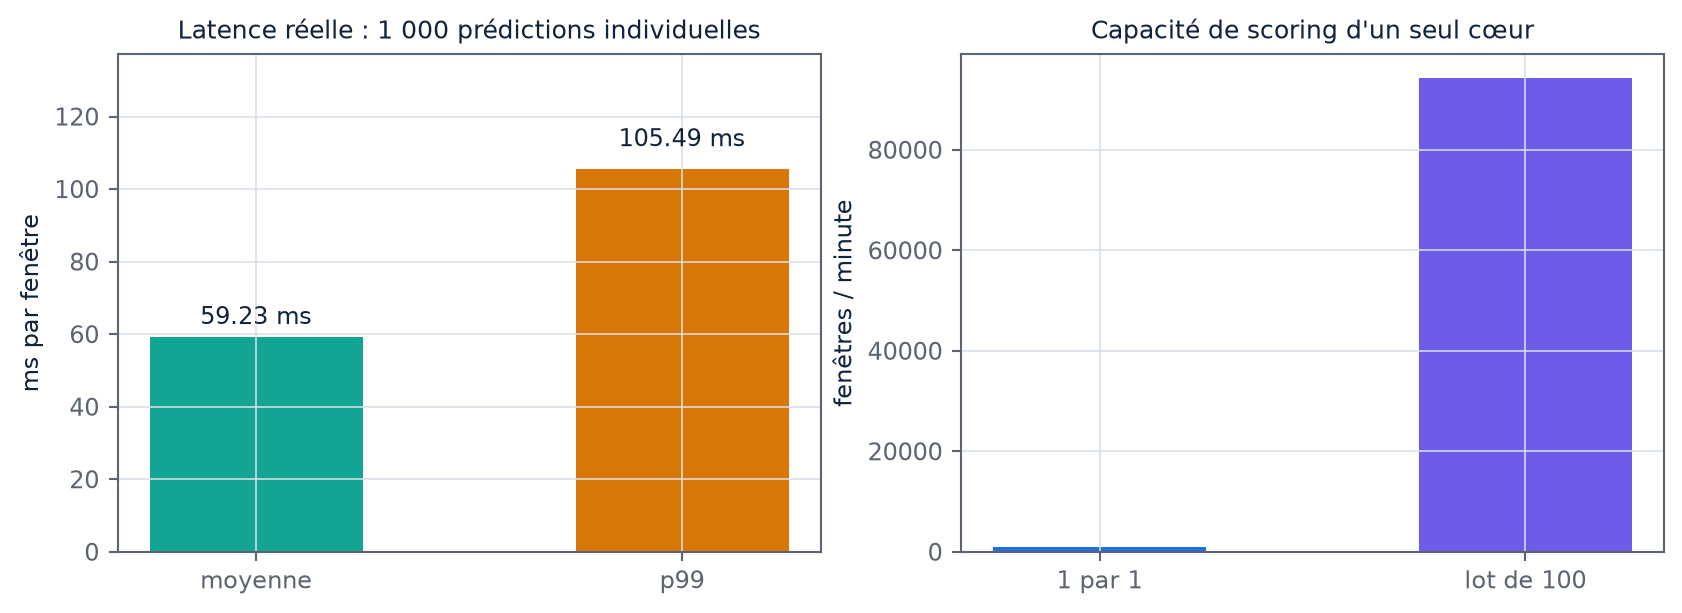
\includegraphics[width=0.62\textwidth]{f34_latence.png}
\end{center}
\begin{columns}[t]
\begin{column}{0.5\textwidth}
\begin{ebox}[Résultats réels du script du cours (1 000 prédictions)]
Moyenne : \textbf{59 ms} par fenêtre --- p99 : \textbf{105 ms}. Par lots de
100 : \textbf{94 279 fenêtres/min} par cœur. Les chiffres de votre machine
seront vos propres mesures --- c'est ça le livrable.
\end{ebox}
\end{column}
\begin{column}{0.46\textwidth}
\begin{qbox}[Le raisonnement de capacité à rédiger]
NOSYS produit \textbf{1 152 fenêtres/jour} (8 serveurs). Un cœur à 1 000
fenêtres/min en individuel : quelle marge ? Et pourquoi le scoring par lots
est-il $\approx$ 90 fois plus rapide par fenêtre ? (indice : overhead
d'appel, parallélisme interne des arbres)
\end{qbox}
\end{column}
\end{columns}
\end{frame}

\begin{frame}{TP B3 --- la fiche MLOps d'une page (30 min)}
\small
\begin{columns}[t]
\begin{column}{0.52\textwidth}
\small\begin{abox}[Les trois rubriques imposées]
\begin{enumerate}
\item \textbf{Plan de retraining} : fréquence de base (ex. hebdomadaire) et
\textbf{déclencheurs chiffrés} --- ex. « proba moyenne $>$ 0,005 pendant
48 h », « taux d'alertes $>$ 0,2 \%», « AUC $<$ 0,70 dès que mesurable ».
\item \textbf{Métriques surveillées} : AUC, taux d'alertes, latence moyenne
+ p99, distribution des entrées --- avec les valeurs réelles du B2 et de f29.
\item \textbf{Procédure de rollback} : garder les N dernières versions ; si
le taux d'alertes double après bascule, revenir à la version précédente en
moins de 10 minutes.
\end{enumerate}
\end{abox}
\end{column}
\begin{column}{0.44\textwidth}
\small\begin{kbox}[Barème B3 (sur 7 pts de la note TP)]
\begin{itemize}
\item Déclencheurs \textbf{chiffrés} et justifiés par les mesures --- 3 pts
\item Métriques complètes avec valeurs réelles --- 2 pts
\item Rollback testable (qui, quoi, délai) --- 2 pts
\end{itemize}
\end{kbox}
\begin{wbox}[Le critère de réussite]
Une fiche MLOps est bonne quand un collègue qui n'a pas suivi le cours
peut faire tourner et surveiller le modèle \textbf{avec elle seule}.
\end{wbox}
\end{column}
\end{columns}
\end{frame}

\begin{frame}{TP B4 --- évaluation blanche : 20 questions (30 min)}
\small
\begin{columns}[t]
\begin{column}{0.52\textwidth}
\begin{ebox}[Format]
QCM identique à l'examen final : \textbf{20 questions}, une par grande
notion : 3 sur les données (séances 1--2), 4 sur classification (séance 3),
3 sur les séries temporelles (séance 4), 3 sur les logs (séance 5),
7 sur MLOps et gouvernance (séance 6).
\end{ebox}
\end{column}
\begin{column}{0.44\textwidth}
\small\begin{kbox}[Exemples de questions]
\begin{enumerate}
\item Le split strict sépare train et test à quelle date ? \hfill (22/09)
\item Pourquoi p99 et pas seulement la moyenne de latence ?\\
(une moyenne cache les rares prédictions très lentes)
\item Que surveille-t-on sur une tranche sans incident ?\\
(la distribution des scores, pas l'AUC)
\end{enumerate}
\end{kbox}
\begin{solbox}[Corrigé]
Distribué après les 30 min --- chaque réponse renvoie à la séance et à la
frame concernée.
\end{solbox}
\end{column}
\end{columns}
\end{frame}

% =====================================================================
%  Seance 6 -- E. Evaluation de l'UE, quiz final, cloture (29--33)
% =====================================================================
\section{Évaluation de l'UE et clôture}

\begin{frame}{Évaluation de l'UE EPD-GIT-5534}
\begin{center}
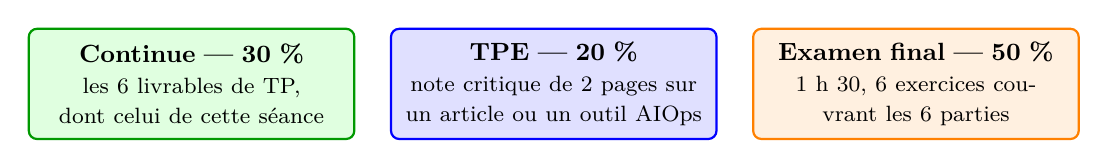
\begin{tikzpicture}[font=\small]
\node[draw=green!60!black, fill=green!12, rounded corners=3pt, thick,
      minimum height=14mm, text width=3.9cm, align=center] at (0,0)
  {\textbf{Continue --- 30 \%}\\ \normalfont\footnotesize les 6 livrables de
   TP, dont celui de cette séance};
\node[draw=blue, fill=blue!12, rounded corners=3pt, thick,
      minimum height=14mm, text width=3.9cm, align=center] at (4.6,0)
  {\textbf{TPE --- 20 \%}\\ \normalfont\footnotesize note critique de 2
   pages sur un article ou un outil AIOps};
\node[draw=orange, fill=orange!12, rounded corners=3pt, thick,
      minimum height=14mm, text width=3.9cm, align=center] at (9.2,0)
  {\textbf{Examen final --- 50 \%}\\ \normalfont\footnotesize 1 h 30,
   6 exercices couvrant les 6 parties};
\end{tikzpicture}
\end{center}
\vspace{2mm}
\begin{columns}[t]
\begin{column}{0.48\textwidth}
\begin{ebox}[TPE : ce qui est attendu]
Deux pages : un article ou un outil AIOps réel (par ex. une lecture sur
l'isolation forest appliquée aux métriques, ou un outil de monitoring),
résumé en 10 lignes + \textbf{votre} critique : que vaut la méthode sur des
données comme NOSYS ?
\end{ebox}
\end{column}
\begin{column}{0.48\textwidth}
\begin{kbox}[Examen final : les 6 exercices]
Un exercice par partie du syllabus : profil des données, préparation,
classification sur classe rare, séries temporelles, logs et sécurité,
industrialisation. Le quiz blanc du B4 en est le miroir exact.
\end{kbox}
\end{column}
\end{columns}
\end{frame}

\begin{frame}{Quiz final de clôture --- 6 QCM sur l'ensemble de l'UE (1/2)}
\begin{qbox}[Questions 1 à 3]
\begin{enumerate}
\item Séance 1--2 --- La première chose à faire devant une valeur
impossible (CPU à 350 \%) est :\\
(a) supprimer la ligne \quad (b) la convertir en manquant avec la borne
physique documentée \quad (c) la garder telle quelle
\item Séance 2 --- Le jeu supervisé contient 120 positives sur 34 560
fenêtres, soit :\\
(a) 3,5 \% \quad (b) 0,35 \% \quad (c) 12 \%
\item Séance 3 --- Sur une classe aussi rare, la métrique à regarder
d'abord est :\\
(a) l'exactitude (accuracy) \quad (b) le couple précision/rappel \quad
(c) le R²
\end{enumerate}
\end{qbox}
\vspace{1mm}
\begin{solbox}[Réponses]
\textbf{1 : b} \quad \textbf{2 : b} \quad \textbf{3 : b} --- l'accuracy
vaut déjà 99,65 \% en prédisant tout « pas d'incident ».
\end{solbox}
\end{frame}

\begin{frame}{Quiz final de clôture --- 6 QCM sur l'ensemble de l'UE (2/2)}
\begin{qbox}[Questions 4 à 6]
\begin{enumerate}
\item Séance 4 --- La validation d'un modèle de prédiction de panne doit
être :\\
(a) croisée aléatoire \quad (b) temporelle, le test strictement après le
train \quad (c) faite sur le train
\item Séance 5 --- La brute force du 5/10 sur \file{bdd-principal} se
détecte par :\\
(a) une hausse du CPU \quad (b) une séquence d'échecs d'authentification
concentrés dans le temps ($\approx$ 125) \quad (c) une baisse de latence
\item Séance 6 --- Sur les tranches de test sans incident, on surveille :\\
(a) l'AUC \quad (b) la distribution des scores et le taux d'alertes \quad
(c) rien
\end{enumerate}
\end{qbox}
\vspace{1mm}
\begin{solbox}[Réponses]
\textbf{4 : b} --- sinon fuite : le modèle aurait « vu » l'avenir \quad
\textbf{5 : b} \quad \textbf{6 : b}
\end{solbox}
\end{frame}

\begin{frame}{Les 6 messages de l'UE}
\begin{kbox}[Si vous ne retenez que six choses]
\begin{enumerate}
\item \textbf{Les données d'infrastructure ont des défauts systématiques} ---
audit avant réparation, granularité et horloges d'abord.
\item \textbf{L'étiquette est le cœur du projet} : « incident $\le$ 30 min »
regardant le futur, sans fuite --- 80 \% des échecs sont là.
\item \textbf{La classe rare impose ses métriques} : précision/rappel et
AUC, jamais l'accuracy.
\item \textbf{Le temps est une contrainte, pas un détail} : split temporel
strict, validation qui respecte la chronologie.
\item \textbf{Les logs complètent les métriques} : l'attaque du 5/10 était
invisible dans les métriques, criante dans les logs.
\item \textbf{Un modèle sans monitoring n'est pas un système} : registre,
latence mesurée, dérive surveillée, rollback écrit.
\end{enumerate}
\end{kbox}
\end{frame}

\begin{frame}{Et après ? --- merci, et la suite du parcours}
\footnotesize%
\begin{columns}[t]
\begin{column}{0.52\textwidth}
\begin{kbox}[Pour continuer seul(e)]
\begin{itemize}
\item \textbf{Deep learning appliqué aux séries temporelles} : réseaux
récurrents, puis les transformers pour la prédiction de charge.
\item \textbf{MLOps avancé} : CI/CD de modèles, déploiement canari,
détection de dérive statistique en continu.
\item \textbf{Certifications cloud} : les services de monitoring des grands
fournisseurs appliquent mot pour mot les concepts de cette UE.
\end{itemize}
\end{kbox}
\end{column}
\begin{column}{0.44\textwidth}
\begin{ebox}[Votre dossier de fin d'UE]
\begin{itemize}
\item \file{nosys\_features.csv} et son dictionnaire.
\item Le pipeline sauvegardé (\file{nosys\_pipeline.joblib}).
\item La fiche MLOps du B3.
\item La note critique TPE.
\end{itemize}
\end{ebox}
\begin{center}\small
Merci pour votre travail sur les six séances ---\\
le prochain système que vous monitorerez vous dira merci aussi.
\end{center}
\end{column}
\end{columns}
\end{frame}

\end{document}
